\documentclass[
	a4paper,					% paper format
	12pt,							% fontsize
	%twoside,					% double-sided
	openright,				% begin new chapter on right side
	notitlepage,			% use no standard title page
	parskip=half,			% set paragraph skip to half of a line
]{article}	

\usepackage[standard-baselineskips]{cmbright}

% Set up page dimension
%---------------------------------------------------------------------------
\usepackage{geometry}
\geometry{
	a4paper,
	left=28mm,
	right=28mm,
	top=30mm,
%	bottom=20mm,
	headheight=20mm,
	headsep=10mm,
	textheight=242mm,
	footskip=15mm
}
%---------------------------------------------------------------------------
\usepackage{pdfpages}
\usepackage{pdflscape}
\usepackage[english]{babel}
\usepackage[utf8]{inputenc}
\usepackage[T1]{fontenc} 
\usepackage{url}
\usepackage{quoting}
\usepackage{placeins}
\usepackage{enumerate}
\usepackage{array}
\usepackage{xurl}

%\usepackage{biblatex}
\usepackage[
backend=biber,
%style=ieee,
%style=unsrt,
sorting=none
]{biblatex}


\addbibresource{database/references.bib}
\DeclareLanguageMapping{english}{UKenglish}
%---------------------------------------------------------------------------	
% Test
\usepackage[breakable]{tcolorbox}
    \usepackage{parskip} % Stop auto-indenting (to mimic markdown behaviour)
    
    \usepackage{iftex}
    \ifPDFTeX
    	\usepackage[T1]{fontenc}
    	\usepackage{mathpazo}
    \else
    	\usepackage{fontspec}
    \fi

    % Basic figure setup, for now with no caption control since it's done
    % automatically by Pandoc (which extracts ![](path) syntax from Markdown).
    \usepackage{graphicx}
    % Maintain compatibility with old templates. Remove in nbconvert 6.0
    \let\Oldincludegraphics\includegraphics
    % Ensure that by default, figures have no caption (until we provide a
    % proper Figure object with a Caption API and a way to capture that
    % in the conversion process - todo).
    %\usepackage{caption}
    %\DeclareCaptionFormat{nocaption}{}
    %\captionsetup{format=nocaption,aboveskip=0pt,belowskip=0pt}

    \usepackage{float}
    \floatplacement{figure}{H} % forces figures to be placed at the correct location
    \usepackage{xcolor} % Allow colors to be defined
    \usepackage{enumerate} % Needed for markdown enumerations to work
    \usepackage{geometry} % Used to adjust the document margins
    \usepackage{amsmath} % Equations
    \usepackage{amssymb} % Equations
    \usepackage{textcomp} % defines textquotesingle
    % Hack from http://tex.stackexchange.com/a/47451/13684:
    \AtBeginDocument{%
        \def\PYZsq{\textquotesingle}% Upright quotes in Pygmentized code
    }
    \usepackage{upquote} % Upright quotes for verbatim code
    \usepackage{eurosym} % defines \euro
    %\usepackage[mathletters]{ucs} % Extended unicode (utf-8) support
    \usepackage{fancyvrb} % verbatim replacement that allows latex
    \usepackage{grffile} % extends the file name processing of package graphics 
                         % to support a larger range
    \makeatletter % fix for old versions of grffile with XeLaTeX
    \@ifpackagelater{grffile}{2019/11/01}
    {
      % Do nothing on new versions
    }
    {
      \def\Gread@@xetex#1{%
        \IfFileExists{"\Gin@base".bb}%
        {\Gread@eps{\Gin@base.bb}}%
        {\Gread@@xetex@aux#1}%
      }
    }
    \makeatother
    \usepackage[Export]{adjustbox} % Used to constrain images to a maximum size
    \adjustboxset{max size={0.9\linewidth}{0.9\paperheight}}

    % The hyperref package gives us a pdf with properly built
    % internal navigation ('pdf bookmarks' for the table of contents,
    % internal cross-reference links, web links for URLs, etc.)
    \usepackage{hyperref}
    % The default LaTeX title has an obnoxious amount of whitespace. By default,
    % titling removes some of it. It also provides customization options.
    \usepackage{titling}
    \usepackage{longtable} % longtable support required by pandoc >1.10
    \usepackage{booktabs}  % table support for pandoc > 1.12.2
    \usepackage[inline]{enumitem} % IRkernel/repr support (it uses the enumerate* environment)
    \usepackage[normalem]{ulem} % ulem is needed to support strikethroughs (\sout)
                                % normalem makes italics be italics, not underlines
    \usepackage{mathrsfs}
    

    
    % Colors for the hyperref package
    \definecolor{black}{rgb}{0,0,0}
    \definecolor{urlcolor}{rgb}{0,.145,.698}
    \definecolor{linkcolor}{rgb}{.71,0.21,0.01}
    \definecolor{citecolor}{rgb}{.12,.54,.11}
    \definecolor{bfhgrey}{rgb}{0.41,0.49,0.57}      % BFH grey

    % ANSI colors
    \definecolor{ansi-black}{HTML}{3E424D}
    \definecolor{ansi-black-intense}{HTML}{282C36}
    \definecolor{ansi-red}{HTML}{E75C58}
    \definecolor{ansi-red-intense}{HTML}{B22B31}
    \definecolor{ansi-green}{HTML}{00A250}
    \definecolor{ansi-green-intense}{HTML}{007427}
    \definecolor{ansi-yellow}{HTML}{DDB62B}
    \definecolor{ansi-yellow-intense}{HTML}{B27D12}
    \definecolor{ansi-blue}{HTML}{208FFB}
    \definecolor{ansi-blue-intense}{HTML}{0065CA}
    \definecolor{ansi-magenta}{HTML}{D160C4}
    \definecolor{ansi-magenta-intense}{HTML}{A03196}
    \definecolor{ansi-cyan}{HTML}{60C6C8}
    \definecolor{ansi-cyan-intense}{HTML}{258F8F}
    \definecolor{ansi-white}{HTML}{C5C1B4}
    \definecolor{ansi-white-intense}{HTML}{A1A6B2}
    \definecolor{ansi-default-inverse-fg}{HTML}{FFFFFF}
    \definecolor{ansi-default-inverse-bg}{HTML}{000000}

    % common color for the border for error outputs.
    \definecolor{outerrorbackground}{HTML}{FFDFDF}

    % commands and environments needed by pandoc snippets
    % extracted from the output of `pandoc -s`
    \providecommand{\tightlist}{%
      \setlength{\itemsep}{0pt}\setlength{\parskip}{0pt}}
    \DefineVerbatimEnvironment{Highlighting}{Verbatim}{commandchars=\\\{\}}
    % Add ',fontsize=\small' for more characters per line
    \newenvironment{Shaded}{}{}
    \newcommand{\KeywordTok}[1]{\textcolor[rgb]{0.00,0.44,0.13}{\textbf{{#1}}}}
    \newcommand{\DataTypeTok}[1]{\textcolor[rgb]{0.56,0.13,0.00}{{#1}}}
    \newcommand{\DecValTok}[1]{\textcolor[rgb]{0.25,0.63,0.44}{{#1}}}
    \newcommand{\BaseNTok}[1]{\textcolor[rgb]{0.25,0.63,0.44}{{#1}}}
    \newcommand{\FloatTok}[1]{\textcolor[rgb]{0.25,0.63,0.44}{{#1}}}
    \newcommand{\CharTok}[1]{\textcolor[rgb]{0.25,0.44,0.63}{{#1}}}
    \newcommand{\StringTok}[1]{\textcolor[rgb]{0.25,0.44,0.63}{{#1}}}
    \newcommand{\CommentTok}[1]{\textcolor[rgb]{0.38,0.63,0.69}{\textit{{#1}}}}
    \newcommand{\OtherTok}[1]{\textcolor[rgb]{0.00,0.44,0.13}{{#1}}}
    \newcommand{\AlertTok}[1]{\textcolor[rgb]{1.00,0.00,0.00}{\textbf{{#1}}}}
    \newcommand{\FunctionTok}[1]{\textcolor[rgb]{0.02,0.16,0.49}{{#1}}}
    \newcommand{\RegionMarkerTok}[1]{{#1}}
    \newcommand{\ErrorTok}[1]{\textcolor[rgb]{1.00,0.00,0.00}{\textbf{{#1}}}}
    \newcommand{\NormalTok}[1]{{#1}}
    
    % Additional commands for more recent versions of Pandoc
    \newcommand{\ConstantTok}[1]{\textcolor[rgb]{0.53,0.00,0.00}{{#1}}}
    \newcommand{\SpecialCharTok}[1]{\textcolor[rgb]{0.25,0.44,0.63}{{#1}}}
    \newcommand{\VerbatimStringTok}[1]{\textcolor[rgb]{0.25,0.44,0.63}{{#1}}}
    \newcommand{\SpecialStringTok}[1]{\textcolor[rgb]{0.73,0.40,0.53}{{#1}}}
    \newcommand{\ImportTok}[1]{{#1}}
    \newcommand{\DocumentationTok}[1]{\textcolor[rgb]{0.73,0.13,0.13}{\textit{{#1}}}}
    \newcommand{\AnnotationTok}[1]{\textcolor[rgb]{0.38,0.63,0.69}{\textbf{\textit{{#1}}}}}
    \newcommand{\CommentVarTok}[1]{\textcolor[rgb]{0.38,0.63,0.69}{\textbf{\textit{{#1}}}}}
    \newcommand{\VariableTok}[1]{\textcolor[rgb]{0.10,0.09,0.49}{{#1}}}
    \newcommand{\ControlFlowTok}[1]{\textcolor[rgb]{0.00,0.44,0.13}{\textbf{{#1}}}}
    \newcommand{\OperatorTok}[1]{\textcolor[rgb]{0.40,0.40,0.40}{{#1}}}
    \newcommand{\BuiltInTok}[1]{{#1}}
    \newcommand{\ExtensionTok}[1]{{#1}}
    \newcommand{\PreprocessorTok}[1]{\textcolor[rgb]{0.74,0.48,0.00}{{#1}}}
    \newcommand{\AttributeTok}[1]{\textcolor[rgb]{0.49,0.56,0.16}{{#1}}}
    \newcommand{\InformationTok}[1]{\textcolor[rgb]{0.38,0.63,0.69}{\textbf{\textit{{#1}}}}}
    \newcommand{\WarningTok}[1]{\textcolor[rgb]{0.38,0.63,0.69}{\textbf{\textit{{#1}}}}}
    
    
    % Define a nice break command that doesn't care if a line doesn't already
    % exist.
    \def\br{\hspace*{\fill} \\* }
    % Math Jax compatibility definitions
    \def\gt{>}
    \def\lt{<}
    \let\Oldtex\TeX
    \let\Oldlatex\LaTeX
    \renewcommand{\TeX}{\textrm{\Oldtex}}
    \renewcommand{\LaTeX}{\textrm{\Oldlatex}}
    % Document parameters
    % Document title
    \title{clean}
    
    
    
    
    
% Pygments definitions
\makeatletter
\def\PY@reset{\let\PY@it=\relax \let\PY@bf=\relax%
    \let\PY@ul=\relax \let\PY@tc=\relax%
    \let\PY@bc=\relax \let\PY@ff=\relax}
\def\PY@tok#1{\csname PY@tok@#1\endcsname}
\def\PY@toks#1+{\ifx\relax#1\empty\else%
    \PY@tok{#1}\expandafter\PY@toks\fi}
\def\PY@do#1{\PY@bc{\PY@tc{\PY@ul{%
    \PY@it{\PY@bf{\PY@ff{#1}}}}}}}
\def\PY#1#2{\PY@reset\PY@toks#1+\relax+\PY@do{#2}}

\expandafter\def\csname PY@tok@w\endcsname{\def\PY@tc##1{\textcolor[rgb]{0.73,0.73,0.73}{##1}}}
\expandafter\def\csname PY@tok@c\endcsname{\let\PY@it=\textit\def\PY@tc##1{\textcolor[rgb]{0.25,0.50,0.50}{##1}}}
\expandafter\def\csname PY@tok@cp\endcsname{\def\PY@tc##1{\textcolor[rgb]{0.74,0.48,0.00}{##1}}}
\expandafter\def\csname PY@tok@k\endcsname{\let\PY@bf=\textbf\def\PY@tc##1{\textcolor[rgb]{0.00,0.50,0.00}{##1}}}
\expandafter\def\csname PY@tok@kp\endcsname{\def\PY@tc##1{\textcolor[rgb]{0.00,0.50,0.00}{##1}}}
\expandafter\def\csname PY@tok@kt\endcsname{\def\PY@tc##1{\textcolor[rgb]{0.69,0.00,0.25}{##1}}}
\expandafter\def\csname PY@tok@o\endcsname{\def\PY@tc##1{\textcolor[rgb]{0.40,0.40,0.40}{##1}}}
\expandafter\def\csname PY@tok@ow\endcsname{\let\PY@bf=\textbf\def\PY@tc##1{\textcolor[rgb]{0.67,0.13,1.00}{##1}}}
\expandafter\def\csname PY@tok@nb\endcsname{\def\PY@tc##1{\textcolor[rgb]{0.00,0.50,0.00}{##1}}}
\expandafter\def\csname PY@tok@nf\endcsname{\def\PY@tc##1{\textcolor[rgb]{0.00,0.00,1.00}{##1}}}
\expandafter\def\csname PY@tok@nc\endcsname{\let\PY@bf=\textbf\def\PY@tc##1{\textcolor[rgb]{0.00,0.00,1.00}{##1}}}
\expandafter\def\csname PY@tok@nn\endcsname{\let\PY@bf=\textbf\def\PY@tc##1{\textcolor[rgb]{0.00,0.00,1.00}{##1}}}
\expandafter\def\csname PY@tok@ne\endcsname{\let\PY@bf=\textbf\def\PY@tc##1{\textcolor[rgb]{0.82,0.25,0.23}{##1}}}
\expandafter\def\csname PY@tok@nv\endcsname{\def\PY@tc##1{\textcolor[rgb]{0.10,0.09,0.49}{##1}}}
\expandafter\def\csname PY@tok@no\endcsname{\def\PY@tc##1{\textcolor[rgb]{0.53,0.00,0.00}{##1}}}
\expandafter\def\csname PY@tok@nl\endcsname{\def\PY@tc##1{\textcolor[rgb]{0.63,0.63,0.00}{##1}}}
\expandafter\def\csname PY@tok@ni\endcsname{\let\PY@bf=\textbf\def\PY@tc##1{\textcolor[rgb]{0.60,0.60,0.60}{##1}}}
\expandafter\def\csname PY@tok@na\endcsname{\def\PY@tc##1{\textcolor[rgb]{0.49,0.56,0.16}{##1}}}
\expandafter\def\csname PY@tok@nt\endcsname{\let\PY@bf=\textbf\def\PY@tc##1{\textcolor[rgb]{0.00,0.50,0.00}{##1}}}
\expandafter\def\csname PY@tok@nd\endcsname{\def\PY@tc##1{\textcolor[rgb]{0.67,0.13,1.00}{##1}}}
\expandafter\def\csname PY@tok@s\endcsname{\def\PY@tc##1{\textcolor[rgb]{0.73,0.13,0.13}{##1}}}
\expandafter\def\csname PY@tok@sd\endcsname{\let\PY@it=\textit\def\PY@tc##1{\textcolor[rgb]{0.73,0.13,0.13}{##1}}}
\expandafter\def\csname PY@tok@si\endcsname{\let\PY@bf=\textbf\def\PY@tc##1{\textcolor[rgb]{0.73,0.40,0.53}{##1}}}
\expandafter\def\csname PY@tok@se\endcsname{\let\PY@bf=\textbf\def\PY@tc##1{\textcolor[rgb]{0.73,0.40,0.13}{##1}}}
\expandafter\def\csname PY@tok@sr\endcsname{\def\PY@tc##1{\textcolor[rgb]{0.73,0.40,0.53}{##1}}}
\expandafter\def\csname PY@tok@ss\endcsname{\def\PY@tc##1{\textcolor[rgb]{0.10,0.09,0.49}{##1}}}
\expandafter\def\csname PY@tok@sx\endcsname{\def\PY@tc##1{\textcolor[rgb]{0.00,0.50,0.00}{##1}}}
\expandafter\def\csname PY@tok@m\endcsname{\def\PY@tc##1{\textcolor[rgb]{0.40,0.40,0.40}{##1}}}
\expandafter\def\csname PY@tok@gh\endcsname{\let\PY@bf=\textbf\def\PY@tc##1{\textcolor[rgb]{0.00,0.00,0.50}{##1}}}
\expandafter\def\csname PY@tok@gu\endcsname{\let\PY@bf=\textbf\def\PY@tc##1{\textcolor[rgb]{0.50,0.00,0.50}{##1}}}
\expandafter\def\csname PY@tok@gd\endcsname{\def\PY@tc##1{\textcolor[rgb]{0.63,0.00,0.00}{##1}}}
\expandafter\def\csname PY@tok@gi\endcsname{\def\PY@tc##1{\textcolor[rgb]{0.00,0.63,0.00}{##1}}}
\expandafter\def\csname PY@tok@gr\endcsname{\def\PY@tc##1{\textcolor[rgb]{1.00,0.00,0.00}{##1}}}
\expandafter\def\csname PY@tok@ge\endcsname{\let\PY@it=\textit}
\expandafter\def\csname PY@tok@gs\endcsname{\let\PY@bf=\textbf}
\expandafter\def\csname PY@tok@gp\endcsname{\let\PY@bf=\textbf\def\PY@tc##1{\textcolor[rgb]{0.00,0.00,0.50}{##1}}}
\expandafter\def\csname PY@tok@go\endcsname{\def\PY@tc##1{\textcolor[rgb]{0.53,0.53,0.53}{##1}}}
\expandafter\def\csname PY@tok@gt\endcsname{\def\PY@tc##1{\textcolor[rgb]{0.00,0.27,0.87}{##1}}}
\expandafter\def\csname PY@tok@err\endcsname{\def\PY@bc##1{\setlength{\fboxsep}{0pt}\fcolorbox[rgb]{1.00,0.00,0.00}{1,1,1}{\strut ##1}}}
\expandafter\def\csname PY@tok@kc\endcsname{\let\PY@bf=\textbf\def\PY@tc##1{\textcolor[rgb]{0.00,0.50,0.00}{##1}}}
\expandafter\def\csname PY@tok@kd\endcsname{\let\PY@bf=\textbf\def\PY@tc##1{\textcolor[rgb]{0.00,0.50,0.00}{##1}}}
\expandafter\def\csname PY@tok@kn\endcsname{\let\PY@bf=\textbf\def\PY@tc##1{\textcolor[rgb]{0.00,0.50,0.00}{##1}}}
\expandafter\def\csname PY@tok@kr\endcsname{\let\PY@bf=\textbf\def\PY@tc##1{\textcolor[rgb]{0.00,0.50,0.00}{##1}}}
\expandafter\def\csname PY@tok@bp\endcsname{\def\PY@tc##1{\textcolor[rgb]{0.00,0.50,0.00}{##1}}}
\expandafter\def\csname PY@tok@fm\endcsname{\def\PY@tc##1{\textcolor[rgb]{0.00,0.00,1.00}{##1}}}
\expandafter\def\csname PY@tok@vc\endcsname{\def\PY@tc##1{\textcolor[rgb]{0.10,0.09,0.49}{##1}}}
\expandafter\def\csname PY@tok@vg\endcsname{\def\PY@tc##1{\textcolor[rgb]{0.10,0.09,0.49}{##1}}}
\expandafter\def\csname PY@tok@vi\endcsname{\def\PY@tc##1{\textcolor[rgb]{0.10,0.09,0.49}{##1}}}
\expandafter\def\csname PY@tok@vm\endcsname{\def\PY@tc##1{\textcolor[rgb]{0.10,0.09,0.49}{##1}}}
\expandafter\def\csname PY@tok@sa\endcsname{\def\PY@tc##1{\textcolor[rgb]{0.73,0.13,0.13}{##1}}}
\expandafter\def\csname PY@tok@sb\endcsname{\def\PY@tc##1{\textcolor[rgb]{0.73,0.13,0.13}{##1}}}
\expandafter\def\csname PY@tok@sc\endcsname{\def\PY@tc##1{\textcolor[rgb]{0.73,0.13,0.13}{##1}}}
\expandafter\def\csname PY@tok@dl\endcsname{\def\PY@tc##1{\textcolor[rgb]{0.73,0.13,0.13}{##1}}}
\expandafter\def\csname PY@tok@s2\endcsname{\def\PY@tc##1{\textcolor[rgb]{0.73,0.13,0.13}{##1}}}
\expandafter\def\csname PY@tok@sh\endcsname{\def\PY@tc##1{\textcolor[rgb]{0.73,0.13,0.13}{##1}}}
\expandafter\def\csname PY@tok@s1\endcsname{\def\PY@tc##1{\textcolor[rgb]{0.73,0.13,0.13}{##1}}}
\expandafter\def\csname PY@tok@mb\endcsname{\def\PY@tc##1{\textcolor[rgb]{0.40,0.40,0.40}{##1}}}
\expandafter\def\csname PY@tok@mf\endcsname{\def\PY@tc##1{\textcolor[rgb]{0.40,0.40,0.40}{##1}}}
\expandafter\def\csname PY@tok@mh\endcsname{\def\PY@tc##1{\textcolor[rgb]{0.40,0.40,0.40}{##1}}}
\expandafter\def\csname PY@tok@mi\endcsname{\def\PY@tc##1{\textcolor[rgb]{0.40,0.40,0.40}{##1}}}
\expandafter\def\csname PY@tok@il\endcsname{\def\PY@tc##1{\textcolor[rgb]{0.40,0.40,0.40}{##1}}}
\expandafter\def\csname PY@tok@mo\endcsname{\def\PY@tc##1{\textcolor[rgb]{0.40,0.40,0.40}{##1}}}
\expandafter\def\csname PY@tok@ch\endcsname{\let\PY@it=\textit\def\PY@tc##1{\textcolor[rgb]{0.25,0.50,0.50}{##1}}}
\expandafter\def\csname PY@tok@cm\endcsname{\let\PY@it=\textit\def\PY@tc##1{\textcolor[rgb]{0.25,0.50,0.50}{##1}}}
\expandafter\def\csname PY@tok@cpf\endcsname{\let\PY@it=\textit\def\PY@tc##1{\textcolor[rgb]{0.25,0.50,0.50}{##1}}}
\expandafter\def\csname PY@tok@c1\endcsname{\let\PY@it=\textit\def\PY@tc##1{\textcolor[rgb]{0.25,0.50,0.50}{##1}}}
\expandafter\def\csname PY@tok@cs\endcsname{\let\PY@it=\textit\def\PY@tc##1{\textcolor[rgb]{0.25,0.50,0.50}{##1}}}

\def\PYZbs{\char`\\}
\def\PYZus{\char`\_}
\def\PYZob{\char`\{}
\def\PYZcb{\char`\}}
\def\PYZca{\char`\^}
\def\PYZam{\char`\&}
\def\PYZlt{\char`\<}
\def\PYZgt{\char`\>}
\def\PYZsh{\char`\#}
\def\PYZpc{\char`\%}
\def\PYZdl{\char`\$}
\def\PYZhy{\char`\-}
\def\PYZsq{\char`\'}
\def\PYZdq{\char`\"}
\def\PYZti{\char`\~}
% for compatibility with earlier versions
\def\PYZat{@}
\def\PYZlb{[}
\def\PYZrb{]}
\makeatother


    % For linebreaks inside Verbatim environment from package fancyvrb. 
    \makeatletter
        \newbox\Wrappedcontinuationbox 
        \newbox\Wrappedvisiblespacebox 
        \newcommand*\Wrappedvisiblespace {\textcolor{red}{\textvisiblespace}} 
        \newcommand*\Wrappedcontinuationsymbol {\textcolor{red}{\llap{\tiny$\m@th\hookrightarrow$}}} 
        \newcommand*\Wrappedcontinuationindent {3ex } 
        \newcommand*\Wrappedafterbreak {\kern\Wrappedcontinuationindent\copy\Wrappedcontinuationbox} 
        % Take advantage of the already applied Pygments mark-up to insert 
        % potential linebreaks for TeX processing. 
        %        {, <, #, %, $, ' and ": go to next line. 
        %        _, }, ^, &, >, - and ~: stay at end of broken line. 
        % Use of \textquotesingle for straight quote. 
        \newcommand*\Wrappedbreaksatspecials {% 
            \def\PYGZus{\discretionary{\char`\_}{\Wrappedafterbreak}{\char`\_}}% 
            \def\PYGZob{\discretionary{}{\Wrappedafterbreak\char`\{}{\char`\{}}% 
            \def\PYGZcb{\discretionary{\char`\}}{\Wrappedafterbreak}{\char`\}}}% 
            \def\PYGZca{\discretionary{\char`\^}{\Wrappedafterbreak}{\char`\^}}% 
            \def\PYGZam{\discretionary{\char`\&}{\Wrappedafterbreak}{\char`\&}}% 
            \def\PYGZlt{\discretionary{}{\Wrappedafterbreak\char`\<}{\char`\<}}% 
            \def\PYGZgt{\discretionary{\char`\>}{\Wrappedafterbreak}{\char`\>}}% 
            \def\PYGZsh{\discretionary{}{\Wrappedafterbreak\char`\#}{\char`\#}}% 
            \def\PYGZpc{\discretionary{}{\Wrappedafterbreak\char`\%}{\char`\%}}% 
            \def\PYGZdl{\discretionary{}{\Wrappedafterbreak\char`\$}{\char`\$}}% 
            \def\PYGZhy{\discretionary{\char`\-}{\Wrappedafterbreak}{\char`\-}}% 
            \def\PYGZsq{\discretionary{}{\Wrappedafterbreak\textquotesingle}{\textquotesingle}}% 
            \def\PYGZdq{\discretionary{}{\Wrappedafterbreak\char`\"}{\char`\"}}% 
            \def\PYGZti{\discretionary{\char`\~}{\Wrappedafterbreak}{\char`\~}}% 
        } 
        % Some characters . , ; ? ! / are not pygmentized. 
        % This macro makes them "active" and they will insert potential linebreaks 
        \newcommand*\Wrappedbreaksatpunct {% 
            \lccode`\~`\.\lowercase{\def~}{\discretionary{\hbox{\char`\.}}{\Wrappedafterbreak}{\hbox{\char`\.}}}% 
            \lccode`\~`\,\lowercase{\def~}{\discretionary{\hbox{\char`\,}}{\Wrappedafterbreak}{\hbox{\char`\,}}}% 
            \lccode`\~`\;\lowercase{\def~}{\discretionary{\hbox{\char`\;}}{\Wrappedafterbreak}{\hbox{\char`\;}}}% 
            \lccode`\~`\:\lowercase{\def~}{\discretionary{\hbox{\char`\:}}{\Wrappedafterbreak}{\hbox{\char`\:}}}% 
            \lccode`\~`\?\lowercase{\def~}{\discretionary{\hbox{\char`\?}}{\Wrappedafterbreak}{\hbox{\char`\?}}}% 
            \lccode`\~`\!\lowercase{\def~}{\discretionary{\hbox{\char`\!}}{\Wrappedafterbreak}{\hbox{\char`\!}}}% 
            \lccode`\~`\/\lowercase{\def~}{\discretionary{\hbox{\char`\/}}{\Wrappedafterbreak}{\hbox{\char`\/}}}% 
            \catcode`\.\active
            \catcode`\,\active 
            \catcode`\;\active
            \catcode`\:\active
            \catcode`\?\active
            \catcode`\!\active
            \catcode`\/\active 
            \lccode`\~`\~ 	
        }
    \makeatother

    \let\OriginalVerbatim=\Verbatim
    \makeatletter
    \renewcommand{\Verbatim}[1][1]{%
        %\parskip\z@skip
        \sbox\Wrappedcontinuationbox {\Wrappedcontinuationsymbol}%
        \sbox\Wrappedvisiblespacebox {\FV@SetupFont\Wrappedvisiblespace}%
        \def\FancyVerbFormatLine ##1{\hsize\linewidth
            \vtop{\raggedright\hyphenpenalty\z@\exhyphenpenalty\z@
                \doublehyphendemerits\z@\finalhyphendemerits\z@
                \strut ##1\strut}%
        }%
        % If the linebreak is at a space, the latter will be displayed as visible
        % space at end of first line, and a continuation symbol starts next line.
        % Stretch/shrink are however usually zero for typewriter font.
        \def\FV@Space {%
            \nobreak\hskip\z@ plus\fontdimen3\font minus\fontdimen4\font
            \discretionary{\copy\Wrappedvisiblespacebox}{\Wrappedafterbreak}
            {\kern\fontdimen2\font}%
        }%
        
        % Allow breaks at special characters using \PYG... macros.
        \Wrappedbreaksatspecials
        % Breaks at punctuation characters . , ; ? ! and / need catcode=\active 	
        \OriginalVerbatim[#1,codes*=\Wrappedbreaksatpunct]%
    }
    \makeatother

    % Exact colors from NB
    \definecolor{incolor}{HTML}{303F9F}
    \definecolor{outcolor}{HTML}{D84315}
    \definecolor{cellborder}{HTML}{CFCFCF}
    \definecolor{cellbackground}{HTML}{F7F7F7}
    

    % prompt
    \makeatletter
    \newcommand{\boxspacing}{\kern\kvtcb@left@rule\kern\kvtcb@boxsep}
    \makeatother
    \newcommand{\prompt}[4]{
        {\ttfamily\llap{{\color{#2}[#3]:\hspace{3pt}#4}}\vspace{-\baselineskip}}
    }
    
    % Prevent overflowing lines due to hard-to-break entities
    \sloppy 
    % Slightly bigger margins than the latex defaults
    
    \geometry{verbose,tmargin=1in,bmargin=1in,lmargin=1in,rmargin=1in}





%---------------------------------------------------------------------------
\usepackage{textcomp}		% additional symbols
\usepackage{ae}																
\usepackage{fancyhdr}		% simple manipulation of header and footer 
\usepackage{etoolbox}		% color manipulation of header and footer
\usepackage{float}			% floating objects
\usepackage{caption}		% for captions of figures and tables
\usepackage{booktabs}		% package for nicer tables
\usepackage{tocvsec2}		% provides means of controlling the sectional numbering

%---------------------------------------------------------------------------	

% Package to facilitate placement of boxes at absolute positions
%---------------------------------------------------------------------------
\usepackage[absolute]{textpos}
\setlength{\TPHorizModule}{1mm}
\setlength{\TPVertModule}{1mm}
%---------------------------------------------------------------------------		

%epigraph
\usepackage{epigraph}
\setlength\epigraphwidth{.8\textwidth}
%\setlength\epigraphrule{0.3pt}
%\setlength \epigraphwidth {\linewidth}
%\setlength \epigraphrule {0pt}
\AtBeginDocument{\renewcommand {\epigraphflush}{center}}
\renewcommand {\sourceflush} {center}
%\usepackage[export]{adjustbox}[2011/08/13]
\usepackage{adjustbox}[2011/08/13]
%---------------------------------------------------------------------------	

%table
%\renewcommand\arraystretch{1.2}
\usepackage{longtable}
\usepackage{multirow}
\setlength{\arrayrulewidth}{0.2mm}
\setlength{\tabcolsep}{12pt}
\renewcommand{\arraystretch}{1.5}
%---------------------------------------------------------------------------	

% Definition of Colors
%---------------------------------------------------------------------------
%\RequirePackage{color}                          % Color (not xcolor!)
%\definecolor{linkblue}{rgb}{0,0,0.8}            % Standard
%\definecolor{darkblue}{rgb}{0,0.08,0.45}        % Dark blue
%\definecolor{bfhgrey}{rgb}{0.41,0.49,0.57}      % BFH grey
%\definecolor{linkcolor}{rgb}{0,0,0.8}     			% Blue for the web- and cd-version!
%\definecolor{linkcolor}{rgb}{0,0,0}        			% Black for the print-version!
%---------------------------------------------------------------------------

% Hyperref Package (Create links in a pdf)
%---------------------------------------------------------------------------
\usepackage{hyperref}
\hypersetup{
    colorlinks=true,
    linkcolor=black,
    filecolor=magenta,      
    urlcolor=linkcolor,
}
%---------------------------------------------------------------------------

%Headers
\usepackage{graphicx}
\usepackage{color}              %this needs to be here also
\usepackage[rightcaption]{sidecap}
%\makeindex[columns=3, title=Alphabetical Index, intoc]
%---------------------------------------------------------------------------
\usepackage[acronym]{glossaries}
%\usepackage[nonumberlist]{glossaries}
\usepackage{glossaries}
\usepackage{glossary-mcols}
\makeglossaries
\renewcommand*{\glspostdescription}{} % Removes dots at the end of each entry.

\newglossaryentry{BibTeX}{name={BibTeX},description={Program for the creation of 	bibliographical references and directories in \TeX or \LaTeX documents}}
\newglossaryentry{Index}{name={Index},description={Index with keywords from text}}



%---------------------------------------------------------------------------
% Makeindex Package
%---------------------------------------------------------------------------
\usepackage{makeidx}                         		% To produce index
\makeindex                                    	% Index-Initialisation
%---------------------------------------------------------------------------

\begin{document}
%\settocdepth{section} %questo divide content da version
\providecommand{\heading}{Title of Thesis}		%  Insert Title of Thesis here				% Title form titel.tex
\providecommand{\versionnumber}{1.2}			%  Hier die aktuelle Versionsnummer eingeben
\providecommand{\versiondate}{07.02.2014}		%  Hier das Datum der aktuellen Version eingeben  				% Version and date version.tex 


% Set up header and footer
%---------------------------------------------------------------------------
\makeatletter
\patchcmd{\@fancyhead}{\rlap}{\color{bfhgrey}\rlap}{}{}		% new color of header
\patchcmd{\@fancyfoot}{\rlap}{\color{bfhgrey}\rlap}{}{}		% new color of footer
\makeatother

\fancyhf{}																		% clean all fields
\fancypagestyle{plain}{												% new definition of plain style	
	\fancyfoot[OR,EL]{\footnotesize \thepage} 	% footer right part --> page number
	\fancyfoot[OL,ER]{\footnotesize \heading, Version \versionnumber, \versiondate}	% footer even page left part 
}

\renewcommand{\sectionmark}[1]{\markboth{\thesection.  #1}{}}
\renewcommand{\headrulewidth}{0pt}				% no header stripline
\renewcommand{\footrulewidth}{0pt} 				% no bottom stripline

\pagestyle{plain}
%---------------------------------------------------------------------------


% Title Page and Abstract
%---------------------------------------------------------------------------
%\thispagestyle{empty}
%%
% Project documentation template
% ===========================================================================
% This is part of the document "Project documentation template".
% Authors: brd3, kaa1
%

\begin{titlepage}


% BFH-Logo absolute placed at (28,12) on A4 and picture (16:9 or 15cm x 8.5cm)
% Actually not a realy satisfactory solution but working.
%---------------------------------------------------------------------------
\setlength{\unitlength}{1mm}
\begin{textblock}{20}[0,0](28,12)
	
\includegraphics[scale=1.0]{images/BFH_Logo_B.png}
\end{textblock}

% Institution / titel / subtitel / authors / experts:
%---------------------------------------------------------------------------
\begin{flushleft}

\vspace*{21mm}

\fontsize{26pt}{40pt}\selectfont 
\heading				\\							% Read heading from file leader/title.tex
\vspace{2mm}

\fontsize{16pt}{24pt}\selectfont\vspace{0.3em}
Place your subheading here 			\\				% Insert subheading
\vspace{5mm}

\fontsize{10pt}{12pt}\selectfont
\textbf{Description of thesis (semester- / Bachelor thesis / etc.)} \\		% Insert text
\vspace{7mm}

% Abstract (eingeben):
%---------------------------------------------------------------------------
\begin{textblock}{150}(28,100)
\fontsize{10pt}{12pt}\selectfont
[Insert short text (abstract) if desired] \\ 
This document serves as a template for the compilation of reports according to the guidelines of the BFH. The template is written in LATEX and supports the automatic writing of various directories, references, indexing and glossaries. This small text is a summary of this document with a length of 4 to max. 8 lines. \\ 
The cover picture may be turned on or off in the lines 157/158 of the file template.tex.
\end{textblock}

\begin{textblock}{150}(28,225)
\fontsize{10pt}{17pt}\selectfont
\begin{tabbing}
xxxxxxxxxxxxxxx\=xxxxxxxxxxxxxxxxxxxxxxxxxxxxxxxxxxxxxxxxxxxxxxx \kill
Degree course:	\> [z.B. Electrical and Communication Engineering]	\\		% insert name of degree course
Authors:		\> [Test Peter, M\"uster R\"os\"a]		\\					% insert names
Tutor:	\> [Dr.~Xxxx Xxxx, Dr.~Yyyy Yyyy]		\\							% insert names
Constituent:	\> [Wwwww AG]					\\							% insert names
Experts:		\> [Dr.~Zzzz Zzzz]				\\							% insert names
Date:			\> \versiondate					\\							% read from file leader/version.tex
\end{tabbing}

\end{textblock}
\end{flushleft}

\begin{textblock}{150}(28,280)
\noindent 
\color{bfhgrey}\fontsize{9pt}{10pt}\selectfont
Berner Fachhochschule | Haute \'ecole sp\'ecialis\'ee bernoise | Bern University of Applied Sciences
\color{black}\selectfont
\end{textblock}


\end{titlepage}

%
% ===========================================================================
% EOF
%

%
% Project documentation template
% ===========================================================================
% This is part of the document "Project documentation template".
% Authors: brd3, kaa1
%

\begin{titlepage}


% BFH-Logo absolute placed at (28,12) on A4 and picture (16:9 or 15cm x 8.5cm)
% Actually not a realy satisfactory solution but working.
%---------------------------------------------------------------------------
\setlength{\unitlength}{1mm}
\begin{textblock}{20}[0,0](28,12)
	
\includegraphics[scale=1.0]{images/BFH_Logo_B.png}
\end{textblock}

\begin{textblock}{154}(28,48)
	\begin{picture}(150,2)
		\put(0,0){\color{bfhgrey}\rule{150mm}{2mm}}
	\end{picture}
\end{textblock}

\begin{textblock}{154}[0,0](28,50)
	
\includegraphics[scale=1.0]{images/placemarker.jpg}			% define cover picture
\end{textblock}

\begin{textblock}{154}(28,135)
	\begin{picture}(150,2)
		\put(0,0){\color{bfhgrey}\rule{150mm}{2mm}}
	\end{picture}
\end{textblock}
\color{black}

% Institution / titel / subtitel / authors / experts:
%---------------------------------------------------------------------------
\begin{flushleft}

\vspace*{115mm}

\fontsize{26pt}{28pt}\selectfont 
\heading				\\							% Read heading from file leader/title.tex
\vspace{2mm}

\fontsize{16pt}{20pt}\selectfont\vspace{0.3em}
Place your subheading here 			\\				% Insert subheading
\vspace{5mm}

\fontsize{10pt}{12pt}\selectfont
\textbf{Description of thesis (semester- / Bachelor thesis / etc.)} \\		% Insert text
\vspace{3mm}

% Abstract (eingeben):
%---------------------------------------------------------------------------
\begin{textblock}{150}(28,190)
\fontsize{10pt}{12pt}\selectfont
[Insert short text (abstract) if desired] \\ 
This document serves as a template for the compilation of reports according to the guidelines of the BFH. The template is written in LATEX and supports the automatic writing of various directories, references, indexing and glossaries. This small text is a summary of this document with a length of 4 to max. 8 lines. \\ 
The cover picture may be turned on or off in the lines 157/158 of the file template.tex.
\end{textblock}

\begin{textblock}{150}(28,225)
\fontsize{10pt}{17pt}\selectfont
\begin{tabbing}
xxxxxxxxxxxxxxx\=xxxxxxxxxxxxxxxxxxxxxxxxxxxxxxxxxxxxxxxxxxxxxxx \kill
Degree course:	\> [z.B. Electrical and Communication Engineering]	\\		% insert name of degree course
Authors:		\> [Test Peter, M\"uster R\"os\"a]		\\					% insert names
Tutor:	\> [Dr.~Xxxx Xxxx, Dr.~Yyyy Yyyy]		\\							% insert names
Constituent:	\> [Wwwww AG]					\\							% insert names
Experts:		\> [Dr.~Zzzz Zzzz]				\\							% insert names
Date:			\> \versiondate					\\							% read from file leader/version.tex
\end{tabbing}

\end{textblock}
\end{flushleft}

\begin{textblock}{150}(28,280)
\noindent 
\color{bfhgrey}\fontsize{9pt}{10pt}\selectfont
Berner Fachhochschule | Haute \'ecole sp\'ecialis\'ee bernoise | Bern University of Applied Sciences
\color{black}\selectfont
\end{textblock}


\end{titlepage}

%
% ===========================================================================
% EOF
%

\setcounter{page}{2}
% Control of versions :
% -----------------------------------------------

\begin{textblock}{180}(15,150)
\color{black}
\begin{huge}
Versions
\end{huge}
\vspace{10mm}

\fontsize{10pt}{18pt}\selectfont
\begin{tabbing}
xxxxxxxxxxx\=xxxxxxxxxxxxxxx\=xxxxxxxxxxxxxx\=xxxxxxxxxxxxxxxxxxxxxxxxxxxxxxxxxxxxxxxxxxxxxxx \kill
Version	\> Date	\> Status			\> Remarks		\\
0.1	\> 01.08.2013	\> Draft		\> Lorem ipsum dolor sit amet	\\	
0.2	\> 21.08.2013	\> Draft		\> Phasellus scelerisque	\\ 
0.3	\> 02.09.2013	\> Draft		\> Donec eget aliquam urna. Lorem ipsum dolor sit amet	\\ 
1.0	\> 26.01.2014	\> Final		\> Lorem ipsum dolor sit ametPhasellus scelerisque, leo sed iaculis ornare 	\\ 
1.1	\> 31.01.2014	\> Correction	\> Layout changed	\\
1.2	\> 07.02.2014	\> Addition		\> Chapter 1.1 extended	\\
\end{tabbing}

\end{textblock}


%---------------------------------------------------------------------------

% Table of contents
%---------------------------------------------------------------------------
\newpage\leavevmode\thispagestyle{plain}\newpage
\tableofcontents
\newpage\leavevmode\thispagestyle{plain}\newpage
%---------------------------------------------------------------------------

% Main part:
%---------------------------------------------------------------------------
\section[Introduction]{Introduction}
\label{chap:introduction}
\epigraph{\centering \textit{“Things like chatbots, machine learning tools, natural language processing, or sentiment analysis are applications of artificial intelligence that may one day profoundly change how we think about and transact in travel and local experiences.”}}{Gillian Tans}

Sentiment Analysis or Opinion Mining is a way of finding out the polarity or strength of the opinion (positive or negative) that is expressed in written text \cite{samuels_news_2020}.\\
It is used in business to understand social sentiment for their brand, a particular product or service.

\subsection[Previous work]{Previous work}
\label{chap:previouswork}
In the last semester, my project partner and I have for the first time stepped into the world of sentiment analysis, making use of various supports such as tutorials, explanations, and lots of research.
We then decided to use all the material we had found to build something of our own, so we built a tool to categorize the sentiment of hotel reviews.
We wanted to split the sentiment of the reviews into 5 categories: from awful to excellent.
At the end of the project, we managed to have an \gls{accuracy} of about 0.48, taking into consideration the 5 categories was a good result.


\subsection[Project description]{Project description}
\label{chap:intropj_desc}
The thesis project I am working on this semester will still be on sentiment analysis. This time the model created will be used to make predictions about newspaper news, to understand the polarity (positive or negative) of an article or the newspaper itself.
A newspaper can change people's way of thinking and mood because of its polarity. That is why it is vital to understand its importance.
By having the polarity of a newspaper, I can also calculate a lot of things such as: the polarity of a newspaper over time, the various categories, and which of these newspapers affect us the most.

\subsection{Motivation}
As already mentioned, this technology allows to crystallize negative and positive feelings from a text. Besides sentiment classification, sentiment analysis brings many other benefits in areas such as marketing and customer satisfaction. Some of these benefits could be, for example:

\begin{itemize}
\item \textbf{Customer classification}\\
sentiment analysis allows customers to be classified according to their emotional mood. This offers the opportunity to find customers who are more willing to buy.
\item \textbf{Chatbot training}\\
With the results of the sentiment analysis tool, it is possible to train chatbots to recognize and respond to specific customer sentiments.
\item \textbf{Scalability and automation}\\
As a digital tool, sentiment analysis can be easily extended or integrated into an automated system.
\end{itemize}

From these points, a strongly increasing tendency regarding the application of sentiment analysis can be assumed. This makes it even more relevant for developers to get to grips with it. From the developer's perspective, learning sentiment analysis also promotes new experiences in areas such as: 

\begin{itemize}
\item Data analytics
\item Data science
\item Machine learning
\item Predictive modelling
\end{itemize}

\subsection[Goal]{Goal}
\label{chap:intro_goal}
The core of this project is with the help of different tools like \gls{Tensorflow} \cite{tensorflow}, \gls{Keras} \cite{noauthor_keras_nodate} and \gls{BERT} \cite{devlin_bert_2019} to create a model that takes text as input and classifies it in “positive” or “negative”. 
To calculate the polarity of the article, I will use different datasets to create different models, in the end I will use the model and dataset that most reflects my purpose.
Unfortunately, due to an impediment, my partner from the previous project was not able to take part in this assignment, which means that I must continue this project alone.
For a matter of timing and difficulty, I have resized the project and the categories on which to make a prediction will no more be 5 as in the last project, but 2.
This model should be available as a single component that can be integrated into arbitrary applications.\\
For the implementation of the project, I have used several websites and tutorials:
\begin{itemize}
    \item Tutorial for \gls{Keras} \cite{tutorial_keras}
    \item Deep-Learning-For-Hackers \cite{git}
    \item Sentiment Analysis with TensorFlow 2 and \gls{Keras} \cite{tutorial}
    \item Deep Learning LSTM for Sentiment Analysis \cite{karikari_deep_2020}
    \item Natural Language Processing and Sentiment Analysis using \gls{Tensorflow} \cite{khan_natural_2020}
    \item Sentiment Analysis: First Steps With Python's NLTK Library \cite{python_sentiment_nodate}
    \item Sentiment Analysis using Deep Learning with \gls{Tensorflow} \cite{pandey_sentiment_2020}
    \item Practical Text Classification With Python and \gls{Keras} \cite{python_practical_nodate}
    \item Classify text with \gls{BERT} \cite{noauthor_classify_nodate}
    \item Text Classification with \gls{BERT} using Transformers for long text inputs \cite{girdhar_text_2020}
    \item Simple Transformers — Multi-Class Text Classification with \gls{BERT}, RoBERTa, XLNet, XLM, and DistilBERT \cite{rajapakse_simple_2019}
    \item Fine-tuning \gls{BERT} with \gls{Keras} and tf.Module \cite{antyukhov_fine-tuning_2020},
    \item The 1cycle policy \cite{gugger_1cycle_nodate},
    \item \gls{Ktrain} tutorials \cite{maiya_amaiyaktrain_2021}.
\end{itemize}


\subsection{Project organization}
Table~\ref{tab:Organisation} describes who occupies which role in our project organization:
\begin{longtable}[ c ]{| m{5cm} | m{5cm}|  m{3cm}|}
 \hline
 \multicolumn{3}{| c |}{\textbf{Project organization}}\\
 \hline
 \textbf{Role in the \newline project organization} & \textbf{Name}  & \textbf{BFH\newline Abbreviation}\\
 \hline
 \endfirsthead
%
 \multicolumn{3}{c}%
 {{\bfseries Table \thetable\ continued from previous page}} \\
 \hline
 \textbf{Role in the \newline project organization} & \textbf{Name}  & \textbf{BFH Abbreviation}\\
 \hline
 \endhead
%
{Tutor}   & {Mascha Kurpicz-Briki}  & {kim3}   \\ \hline
{Expert}  & {Andreas Dürsteler}         & {-}   \\ \hline
{Developer}     & {Giorgio Bakhiet Derias}& {bakhg1}\\ \hline
                 
\caption{Project organization}
\label{tab:Organisation}\\
\end{longtable}

\subsection{Tools}
\label{chap:intro_tools}
In Table~\ref{tab:Tools} is possible to find the different tools I used for this project:
\begin{longtable}[ c ]{| m{4cm} | m{10cm}|}
 \hline
 \multicolumn{2}{| c |}{\textbf{Tools}}\\
 \hline
 \textbf{Tool}  & \textbf{Description}\\
 \hline
 \endfirsthead
%
 \multicolumn{2}{c}%
 {{\bfseries Table \thetable\ continued from previous page}} \\
 \hline
\textbf{Tool}  & \textbf{Description}\\
 \hline
 \endhead
%
{\gls{jupyter}}           & {A document that can store code, diagrams, graphics and much more.}      \\ \hline
{Google   \gls{colab}oratory} & {Online platform to host \gls{jupyter}.} \\ \hline
{\gls{kaggle}}   & {Is an online machine learning environment and community.}      \\ \hline  
{\gls{anaconda}}          & {Application to manage libraries of larger projects.}      \\ \hline
{\gls{virtual machine}}   & {\gls{anaconda} is installed on the virtual machine to run the project.}      \\ \hline
{PyCharm}   & {IDE used for the Python language. It is developed by the company JetBrains.}      \\ \hline
{GitHub}   & {GitHub is a hosting service for software projects.}      \\ \hline
{\gls{Overleaf}}   & {\gls{Overleaf} is a cloud-based collaborative LaTeX editor used to write, edit, and publish scientific papers.}      \\ \hline
{\gls{MLMP}}   & {\gls{MLMP} is a cloud-based environment for machine learning created by BFH.}      \\ \hline
{\gls{Scikit-learn}}           & {Open-source machine learning software library for the Python programming language.}      \\ \hline
{\gls{Tensorflow}}   & {Open-source software library for machine learning.}      \\ \hline
{\gls{Pandas}}   & {Open-source data analysis and tool for data manipulation, built in Python.}      \\ \hline
{\gls{Keras}}             & {\gls{Tensorflow} library specifically for creating neural networks.}      \\ \hline
{\gls{Ktrain}}   & {\gls{Ktrain} is a library used to build, train, debug, and deploy neural networks in the deep learning software framework \gls{Keras}.}      \\ \hline
{\gls{BERT}}   & {Is a recent paper published by researchers at Google AI Language.}      \\ \hline
{\gls{Hugging Face}}   & {Is an open-source provider of natural language processing (NLP) technologies.} \\ \hline
{\gls{Plotly}}   & {\gls{Plotly} provides online graphing, analytics, and statistics tools for individuals and collaboration, and libraries for Python, R, MATLAB, Perl, Julia, Arduino, and REST.}   \\ \hline

 

\caption{Tools}
\label{tab:Tools}\\
\end{longtable}

\subsection{Project pipeline}
The Project pipeline is shown in Figure~\ref{fig:fig_pipeline}, the pipeline goes from top to bottom.
The pipeline is categorized by color, in fact each color is a key component of the project:
\begin{itemize}
    \item in orange there is the part that concerns the creation of the dataset (Chap:\ref{chap:dataset},\ref{chap:work on dataset}),
    \item in red the part related to \gls{Ktrain} (Chap:\ref{chap:Ktrain model}),
    \item orange and red together will create the model (Chap:\ref{chap:model training}),
    \item in green the data coming from the APIs, this data will be given to the trained model to make predictions (Chap:\ref{chap:model test newspaper}),
    \item in blue the components related to the calculation of polarity, analysis of results and creation of visualization (Chap:\ref{chap:model plot}). 
\end{itemize}
  
\begin{figure}[ht!]
\centering
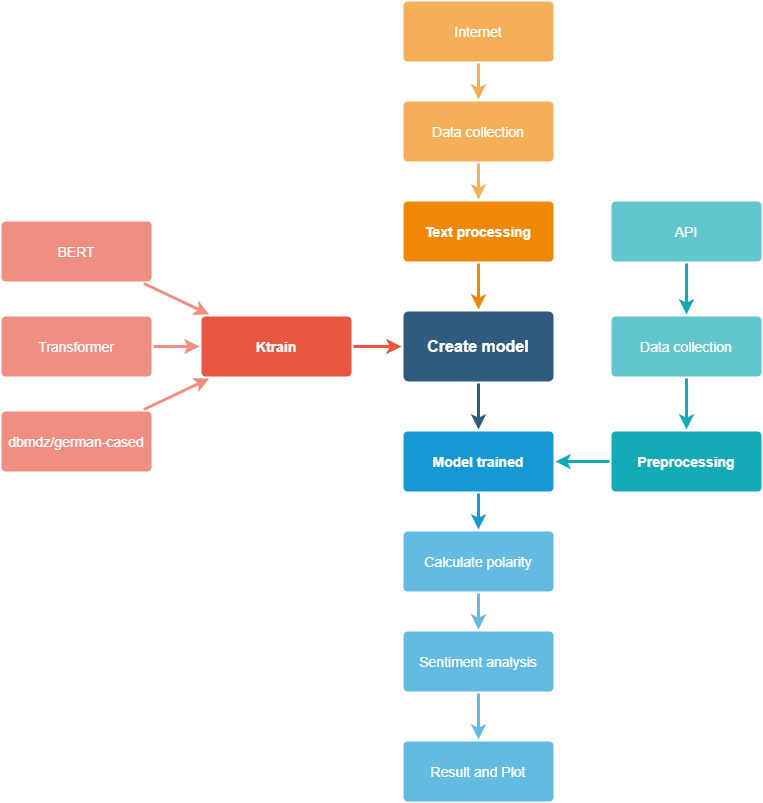
\includegraphics[width=0.9\textwidth]{images/test1.png}
\caption{Project pipeline}
\label{fig:fig_pipeline}
\end{figure}
\FloatBarrier
\section{Technology and setup}
\label{chap:tech}
This section will explain all the components used for the development environment. 
\subsection{Jupyter Notebook}
The model is developed in the form of a \gls{jupyter} \cite{noauthor_project_nodate} using the Python programming language. \gls{jupyter}s are documents that can contain code, text, images, diagrams and explanations. This is especially suitable for this project, because in Machine Learning it is often useful to explain the source code with graphs and diagrams.

\subsection{Google Colaboratory}
The notebook was initially hosted on Google \gls{colab}oratory \cite{colab}. This brought the following advantages:
\paragraph{Synchronization} 
By storing the notebook in a central location, Google Drive, and having everyone access the same notebook, all changes are immediately visible to all users of the notebook.
\paragraph{Project structure} 
The \gls{jupyter} allows to map the whole project in a structured way in a single file. 
\paragraph{Project dependencies}
Since the project is hosted on Google \gls{colab}, it is not necessary as a developer to install libraries and other dependencies locally.

However, as it turned out, \gls{colab} removes from the platform external resources that were imported into the project after a certain time. This meant that I had to re-import the datasets, which are essential for the development of my model, before each work. This forced me to set up a \gls{virtual machine} on which the notebook can then be run locally.

\subsection{Virtual machine}
To have the tools installed in one place, I opted for a virtual machine.
Not only this, the VM has precisely other advantages, which are:
\begin{itemize}
    \item more computing power
    \item do not use my local machine 
    \item is always on, so it can always work
    \item the models are trained on a special machine with special software
    \item being online I can work from any location
    \item always working I can train my models also at night
    \item if by chance something goes wrong, I can backup and create another VM
\end{itemize}

\subsection{Kaggle}
What is Kaggle \cite{noauthor_kaggle_nodate}? 
As it is possible to find written in the documentation: 
\begin{quote}
    "Kaggle is an AirBnB for Data Scientists - this is where they spend their nights and weekends." – Zeeshan-ul-hassan Usmani \cite{zeeshan-ul-hassan_what_2018}
\end{quote}
Founded in 2010 by Anthony Goldbloom (CEO) and Ben Hamner (CTO), and acquired by Google in 2017, Kaggle enables data scientists and other developers to engage in running machine learning contests, write and share code, and to host datasets. 

Kaggle is an online community for data scientists that offers:
\begin{itemize}
    \item machine learning competitions,
    \item datasets,
    \item notebooks,
    \item access to training accelerators,
    \item education.
\end{itemize}
Thanks to its 35k datasets, Kaggle is the perfect place to start a search for a datasets, notebooks or information.

\subsection{Anaconda}
\gls{anaconda} \cite{anaconda_inc_anaconda_nodate} is a distribution of the Python and R programming languages, used for data science, machine learning etc.
\gls{anaconda} is used to simplify package management and deployment of various libraries.
To run \gls{jupyter} with all the needed libraries, \gls{anaconda} has turned out to be a suitable solution. \gls{anaconda} is a platform that allows to set up large projects locally by creating so-called "environments" that contain all the required configurations and libraries for the project. To my advantage, \gls{anaconda} already provides a pre-built environment for \gls{jupyter} projects, which is already equipped with all my needed tools, as shown in Figure~\ref{fig:fig_01}.

\begin{figure}[ht!]
\centering
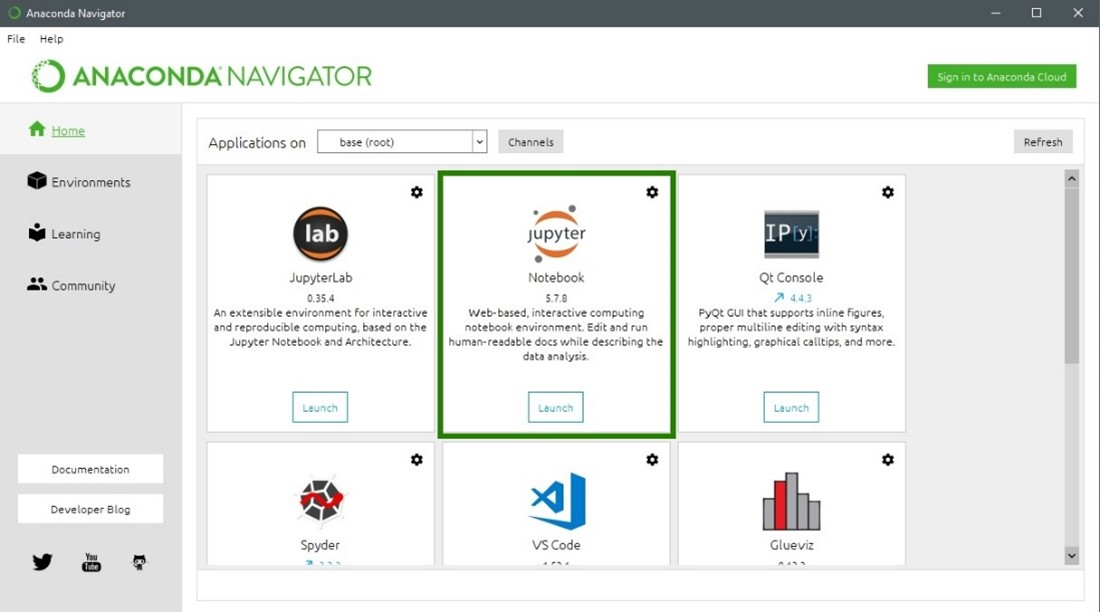
\includegraphics[width=1\textwidth]{images/anaconda.jpg}
\caption{\gls{anaconda} Navigator}
\label{fig:fig_01}
\end{figure}
\FloatBarrier

Theoretically, it would also have been possible for each developer to install \gls{anaconda} on their computer and work on the notebook, which is maintained on a \gls{GitHub} repository. However, since the project is very hardware-heavy and compiling a machine learning model can take up to several hours, a \gls{virtual machine} turns out to be the better option.

\subsection{PyCharm}
\gls{PyCharm} \cite{jetbrains_sro_pycharm_nodate} is an integrated development environment (IDE) used for programming in the Python language, created by the Czech company JetBrains. I used it because it supports anaconda, \gls{GitHub} and as a debugger.
It natively supports jupyter notebooks is perfect because it is much more comfortable than jupyter itself, then it has several extensions that make programming easier and more intuitive.

\subsection{Github}
\gls{GitHub} \cite{github_inc_github_nodate} is a provider with the function of hosting for software development and version control using Git.
Thanks to its free of charge nature it is used for most of the open-source projects.
That is why it is loved by the community of programmers, even I use it for this project to save files and use them from different locations.


\subsection{Overleaf}
\gls{Overleaf} \cite{noauthor_overleaf_nodate} is cloud-based \LaTeX{} editor, which makes writing a scientific paper collaborative. \LaTeX{} is a software widely used in the academic world to create scientific texts, with useful formatting for mathematical, statistical, computer science, physics texts, which can be problematic on other text editors.
I preferred \gls{Overleaf} to other solutions for the convenience, in fact there is no need to install anything, everything is accessible via the internet as with Colab.
\gls{Overleaf} was useful for me to write this documentation, thanks also to its versioning nature.

\subsection{MLMP}
\gls{MLMP} \cite{berner_fachhochschule_mlmp_nodate} is a cloud-based environment in which machine learning models can be trained. Similar to Colab, this environment was created by Department of Engineering and Information Technology of the Bern University of Applied Sciences (BFH), to allow its students to be able to train models, with a more performing machine. It is possible to use it in the BFH network or through a connection to the network via VPN, the advantage lies in being able to use not only the CPU, as in normal virtual machines, but also very powerful GPUs, designed precisely for this purpose.This way I can train my model much faster, having much more computing power at my disposal.

Figure~\ref{fig:fig_02} shows the available environments on \gls{MLMP}:
\begin{figure}[ht!]
\centering
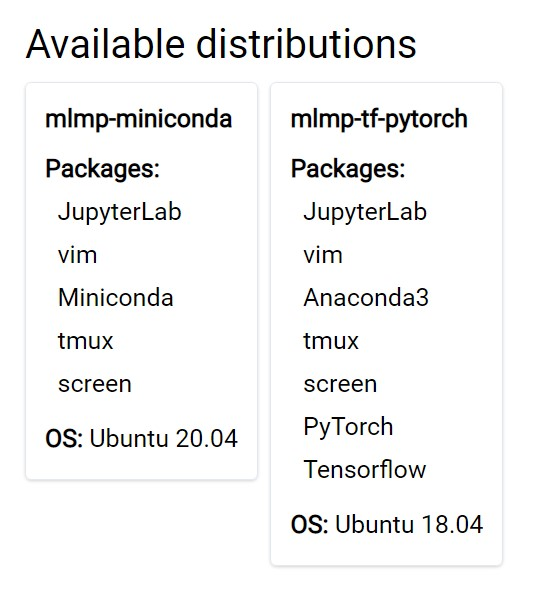
\includegraphics[width=0.5\textwidth]{images/bfhmlmp.jpg}
\caption{\gls{MLMP} distributions}
\label{fig:fig_02}
\end{figure}
\FloatBarrier
\textbf{Which distribution to use?}
To work I chose the distribution \textbf{mlmp-tf-pytorch} because it has the most suitable components for the work I need to do such as: \gls{Tensorflow} and \gls{anaconda} in full version.

As can be seen from this blog \cite{giphy_blown_nodate} the GPU takes much less time to work than the CPU.

\subsection{Scikit-learn}
Scikit-learn \cite{noauthor_scikit-learn_nodate} is a free machine learning library for Python programming language. It features various classification, regression and clustering algorithms including support vector machines, random forests, gradient boosting, k-means and DBSCAN, and is designed to interoperate with the Python numerical and scientific libraries NumPy and SciPy.

\subsection{Pandas}
\gls{Pandas} \cite{noauthor_pandas_nodate} ("Python Data Analysis Library") is an open-source library written in Python, for data analysis and data manipulation tasks.
\gls{Pandas} can be useful for example:
\begin{itemize}
    \item Convert Python lists or dictionaries, Numpy arrays, to \gls{Pandas} data frames.
    \item Inspecting data frames with a lot of functions.
    \item Data manipulation like filter, sort or group by and also data cleaning.
    \item Import local datasets that can be in different formats like CSV, TSV, Excel, etc.
    \item Access remote files or CSV databases or even websites in JSON format or read SQL tables or database.
\end{itemize}

\subsection{Tensorflow}
\gls{Tensorflow} \cite{noauthor_tensorflow_nodate} is a machine learning framework from Google, which facilitates the process of capturing data, training models, making predictions, and refining future results.

\gls{Tensorflow} is an open-source library for large-scale numerical computing and machine learning, it bundles a number of machine learning and deep learning algorithms and models.
All this is provided through the Python language; since it is easy to learn and implement. The actual mathematical operations, however, are performed in high-performance C++.

\subsection{Keras}
\gls{Keras} \cite{noauthor_keras_nodate} is an open-source software library that provides a Python interface for artificial neural networks. \gls{Keras} acts as an interface for the \gls{Tensorflow} library.

A model with \gls{Keras} consists of multiple layers, each of them performs a new data transmutation on the result from the layer above, at the end we will have a series of layers connected like a neural network.

Neural networks do not process raw data, like text files, encoded JPEG image files, or CSV files. They process vectorized and standardized representations.

For this reason, \gls{Keras} comes to our support, in fact we can use \gls{Keras} for all those tasks of data loading and data preprocessing.

Not only this, with \gls{Keras} can also perform many other tasks such as:
\begin{itemize}
    \item Build a model
    \item Train a model with the method fit()
    \item Evaluate a model
    \item Customize the method fit() for fine-tuning
\end{itemize}
See references for more details \cite{team_keras_nodate}

\subsection{BERT}
\gls{BERT} \cite{devlin_bert_2019} (Bidirectional Encoder Representations from Transformers) is an open-source deep learning model developed by Google and stat of the art for NLP tasks.

The biggest difficulty is finding the part of \gls{BERT} that suits best.
In fact, this task needed a lot of time and research to be able to figure out which \gls{BERT} is the right one for this project.

In the list below are the different versions there are of \gls{BERT}:

\begin{itemize}
    \item \gls{BERT}-Base, uncased and seven more models with trained weights released by the original \gls{BERT} authors.
    \item Small BERTs have the same general architecture but fewer and/or smaller Transformer blocks, which lets to explore tradeoffs between speed, size and quality.
    \item ALBERT \cite{lan_albert_2020}: four different sizes of "A Lite \gls{BERT}" that reduces model size (but not computation time) by sharing parameters between layers.
    \item \gls{BERT} Experts \cite{smit_chexbert_2020}: eight models that all have the \gls{BERT}-base architecture but offer a choice between different pre-training domains, to align more closely with the target task.
    \item ELECTRA \cite{clark_electra_2020} has the same architecture as \gls{BERT} (in three different sizes), but gets pre-trained as a discriminator in a set-up that resembles a Generative Adversarial Network (GAN).
    \item \gls{BERT} with Talking-Heads Attention \cite{shazeer_talking-heads_2020} and Gated GELU \cite{shazeer_glu_2020} [base, large] has two improvements to the core of the Transformer architecture.
\end{itemize}
    
\paragraph{How \gls{BERT} works?} \gls{BERT} uses Transformer, that learns contextual relations between words in a text.
Transformer is divided in two different mechanism:
\begin{itemize}
    \item encoder - that reads the text input,
    \item decoder - that produces a prediction.
\end{itemize}
The detailed workings of Transformer are described in a paper by Google \cite{vaswani_attention_2017}.

Transformer encoder reads the entire sequence of words at once. 

\paragraph{\gls{BERT} and Fine-tuning} \gls{BERT} can be used for a wide variety of language tasks, while only adding a small layer to the core model, for classification tasks like sentiment analysis one only needs to add a layer on top of the Transformer output.

\subsection{Ktrain}
\gls{Ktrain} \cite{maiya_amaiyaktrain_2021} is a lightweight wrapper open-source for the deep learning library \gls{Tensorflow} \gls{Keras}, and many pre-trained deep learning architectures like \gls{BERT}.
\gls{Ktrain} helps to build, train, and deploy neural networks and other machine learning models. 
It is designed to make deep learning and AI more accessible and easier to apply for both newcomers and experienced practitioners.

For my task, I will use the implementation of pre-trained \gls{BERT} provided by \gls{Ktrain} and fine-tune it to classify the sentiment of the reviews.


\subsection{Hugging Face}
The \gls{Hugging Face} transformers package is a very popular Python library, that provides thousands of pre-trained models for task text classification, information extraction, question answering, etc. in more than 100 languages.
Thanks to \gls{Hugging Face} NLP has become easy and accessible for everyone.
As of 2019, it also supports Tensorflow2 and not just PyTorch \cite{noauthor_pytorch_nodate} as before.
More information about Hugging Face \cite{noauthor_hugging_nodate}, the related paper \cite{wolf-etal-2020-transformers} and its source code \cite{noauthor_huggingfacetransformers_2021}.

\subsection{Plotly}
\gls{Plotly} \cite{noauthor_plotly_nodate} is a company that develops tools for creating data visualizations for data analysis.
It is also possible to have these tools online for statistical data for individuals or collaborations.
It has a library of different plots \cite{noauthor_plotly_nodate-1} and it is also possible to create dashboards thanks to \gls{Plotly} Dash \cite{noauthor_dash_nodate}.
Having Python compatible libraries was easy for me to import into my Jupyter Notebooks.
\section{The \gls{dataset}s}
\label{chap:dataset}
The most complicated step to start with is to search for a dataset, it is the crucial part because a wrong dataset means a wrongly trained model, so searching for the dataset is crucial and takes a lot of time.
Being in fact so important I spent several hours to research, analyze different datasets, to finally find what I needed.
Initially for my work I chose the IMDb dataset, but not being ideal I then replaced it with the Hotel Review dataset. The problem with both datasets is that they are in English, and it turn out in the project that the articles were in German. I had to search for a dataset in German, and I found the Filmstarts one.

\subsection{IMDB Review Description}
"Large Movie Review Dataset" \cite{noauthor_sentiment_nodate} is a dataset about movie reviews, consisting of 50k reviews which are divided into positive and negative reviews (no neutral).
This is a very famous and used dataset in the world of sentiment classification, other information can be found through the publication "Learning Word Vectors for Sentiment Analysis" \cite{maas-EtAl:2011:ACL-HLT2011}.

\subsubsection*{Motivation of the choice}
When we already have a categorization, we can say we have a labelled dataset.
Having an already labelled dataset, I will not have to do any particular operation, I have just to remove the data that do not interest me. Another advantage is that with tensorflow this dataset is particularly good for the methods I can use that we will see later.

\subsection{Hotel Review Description}
The dataset consists of approximately 515,000 customer reviews on over 1493 luxury hotels throughout Europe. Each review has a score ranging from 1 to 10. The dataset \cite{515k_kaggle} is hosted on \gls{kaggle} and is provided by Jiashen Liu.

\subsubsection*{Motivation of the choice}
The dataset provides an optimal set of datasets for the project. These are provided with plenty of attributes. The structure of the datasets is kept very simple and understandable. Furthermore, \gls{kaggle} has rated this \gls{dataset} with a usability score of 8.2.

\subsection{Filmstarts Description}
The Filmstarts dataset \cite{guhr_oliverguhrgerman-sentiment_2021} consists of 71,229 user written movie reviews in the German language. The dataset is a collection from the German website "filmstarts.de". The users can label their reviews in the range of 0.5 to 5 stars. With 40,049 documents the majority of the reviews in this data set are positive and only 15,610 reviews are negative.

\subsubsection*{Motivation of the choice}
The choice of this dataset fell on the German language, unfortunately there are not many datasets in this language. Fortunately having a score already made it easier to define a sentiment.

\section{Work on the datasets}
\label{chap:work on dataset}
\subsection{Filmstarts Dataset}
\subsubsection*{Dataframe structure}
The dataset is a tab-separated values (TSV) file. A TSV file is a simple text format for storing data in a tabular structure.

First, I need to import the file using pandas, without importing lines with errors:

    \begin{tcolorbox}[breakable, size=fbox, boxrule=1pt, pad at break*=1mm,colback=cellbackground, colframe=cellborder]
\begin{Verbatim}[commandchars=\\\{\},fontsize=\footnotesize]
\PY{c+c1}{\PYZsh{} Load the data using pandas}
\PY{n}{film\PYZus{}de} \PY{o}{=} \PY{n}{pd}\PY{o}{.}\PY{n}{read\PYZus{}csv}\PY{p}{(}\PY{l+s+s2}{\PYZdq{}}\PY{l+s+s2}{filmstarts.tsv}\PY{l+s+s2}{\PYZdq{}}\PY{p}{,} \PY{n}{sep} \PY{o}{=} \PY{l+s+s1}{\PYZsq{}}\PY{l+s+se}{\PYZbs{}t}\PY{l+s+s1}{\PYZsq{}}\PY{p}{,}\PY{n}{encoding}\PY{o}{=}\PY{l+s+s1}{\PYZsq{}}\PY{l+s+s1}{utf8}\PY{l+s+s1}{\PYZsq{}}\PY{p}{,} \PY{n}{error\PYZus{}bad\PYZus{}lines}\PY{o}{=}\PY{k+kc}{False}\PY{p}{,} \PY{n}{warn\PYZus{}bad\PYZus{}lines}\PY{o}{=}\PY{k+kc}{True}\PY{p}{,} \PY{n}{header}\PY{o}{=}\PY{k+kc}{None}\PY{p}{)}
\end{Verbatim}
\end{tcolorbox}

The TSV file contains 3 columns, this means that one customer rating contains 3 attributes. In Table~\ref{tab:Dataframe structure F} all attributes are explained in detail:

\begin{longtable}[ c ]{| m{5cm} | m{8cm}|}
\hline
\multicolumn{2}{|c|}{\textbf{Dataframe structure}}                                                                                                         \\ \hline
\endfirsthead
%
\multicolumn{2}{c}%
{{\bfseries  Table \thetable\ continued from previous page}} \\
\hline
\multicolumn{2}{|c|}{\textbf{Dataframe structure}}                                                                                                         \\ \hline
\endhead
%
\textbf{ 0 }    & Url of the review.\\ \hline
\textbf{ 1 }    & Score Rating.\\ \hline
\textbf{ 2 }    & Text of the review.\\ \hline

\caption{Dataframe structure}
\label{tab:Dataframe structure F}\\
\end{longtable}

\subsubsection{Create an Input and Response Dataframe}
I cleaned the dataframe to remove all the columns that I did not need.
After that I renamed the columns and reordered.
    \begin{tcolorbox}[breakable, size=fbox, boxrule=1pt, pad at break*=1mm,colback=cellbackground, colframe=cellborder]
\begin{Verbatim}[commandchars=\\\{\},fontsize=\small]
\PY{n}{film\PYZus{}de} \PY{o}{=} \PY{n}{film\PYZus{}de}\PY{o}{.}\PY{n}{rename}\PY{p}{(}\PY{n}{columns}\PY{o}{=}\PY{p}{\PYZob{}}\PY{l+m+mi}{2}\PY{p}{:} \PY{l+s+s1}{\PYZsq{}}\PY{l+s+s1}{Review}\PY{l+s+s1}{\PYZsq{}}\PY{p}{,} \PY{l+m+mi}{1}\PY{p}{:} \PY{l+s+s1}{\PYZsq{}}\PY{l+s+s1}{Score}\PY{l+s+s1}{\PYZsq{}}\PY{p}{\PYZcb{}}\PY{p}{)}
\end{Verbatim}
\end{tcolorbox}

            \begin{tcolorbox}[breakable, size=fbox, boxrule=.5pt, pad at break*=1mm, opacityfill=0]
\begin{Verbatim}[commandchars=\\\{\},fontsize=\footnotesize]
                                                  Review  Score
10                                    alle teile gemeint    0.0
11     ALSO:    Ich habe in meinem Leben schon viel S{\ldots}    0.0
55     der Vermarktung!     Ich frage mich allen Erns{\ldots}    1.0
58     Ey isch hab gestern Lordof the Weed gesehen ne{\ldots}    0.0
73     Also ich muss ehrlich sagen das ich es total l{\ldots}    1.0
{\ldots}                                                  {\ldots}    {\ldots}
71073  Zwei Stunden Lebenszeit vergeudet. Hier wird v{\ldots}    0.0
71078  Traumfrauen. Für viele von uns unerreichbar, e{\ldots}    1.0
71081  So einen drecks film sorry aber mir fällt leid{\ldots}    0.0

[7744 rows x 2 columns]
\end{Verbatim}
\end{tcolorbox}

Now that I have cleaned up the dataframes with what I needed, I see how they are composed, as can be seen from the chart in Figure~\ref{fig:fig_03} :

\begin{figure}[H]
\centering
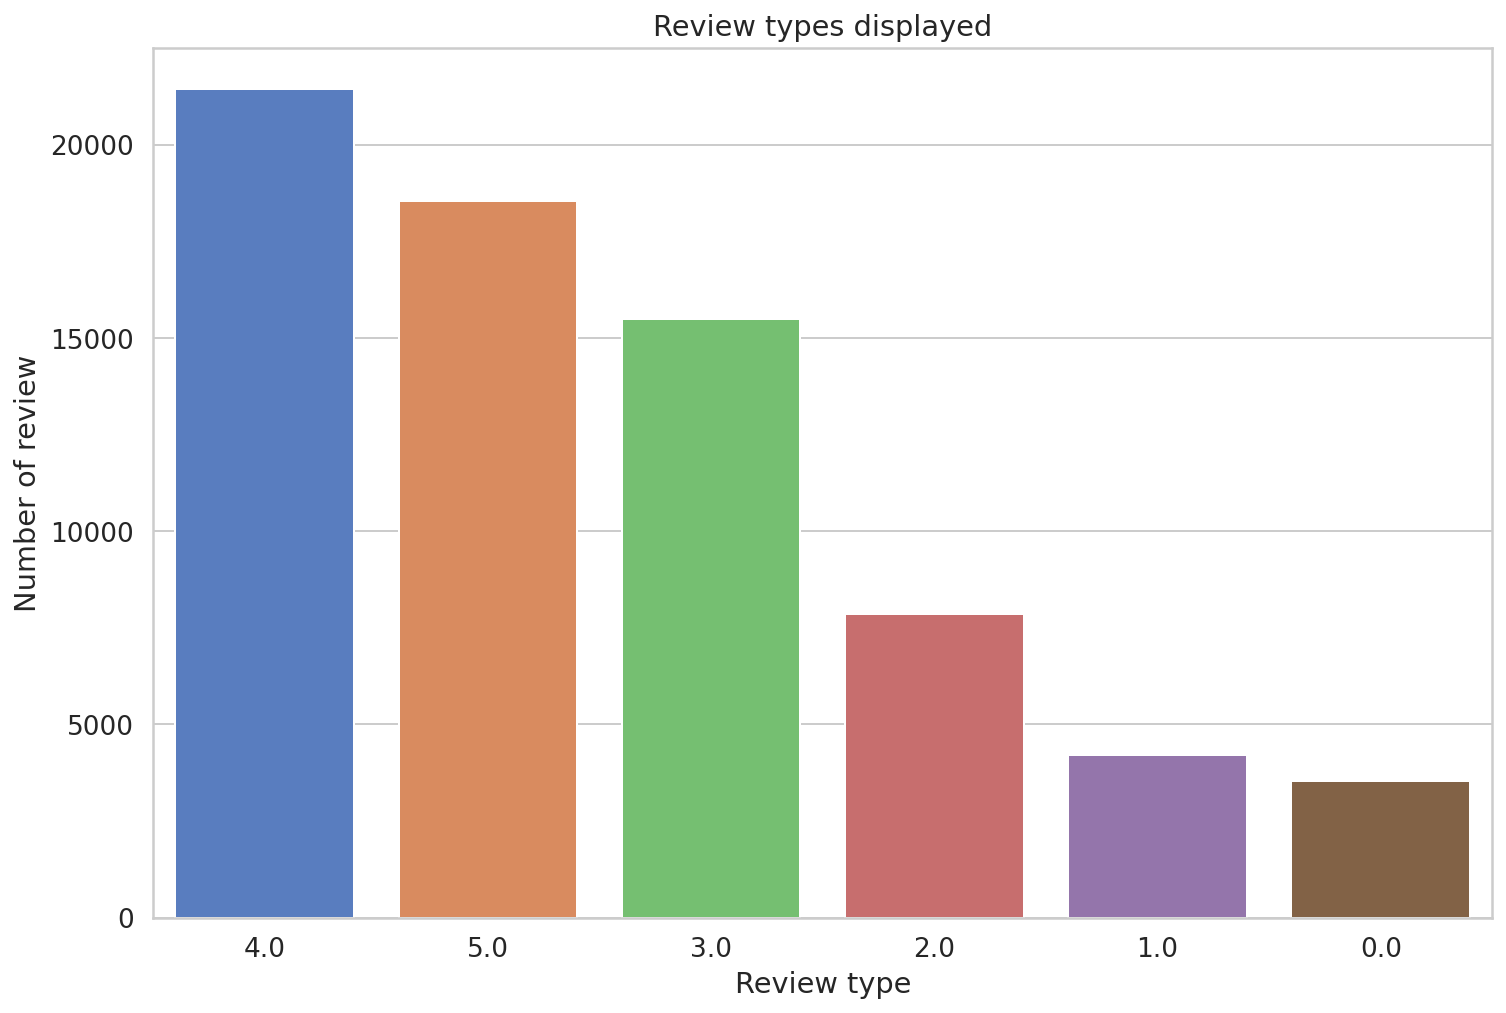
\includegraphics[width=1\textwidth]{images/output_37_1.png}
\caption{Number of ratings per category}
\label{fig:fig_03}
\end{figure}
\FloatBarrier


The "Polarity" of a review is determined by the following criteria:
\begin{itemize}
\item \textbf{"0"}: up to Score 0
\item \textbf{"1"}: up to Score 5
\end{itemize}
The code for this operation is shown here below:

        \begin{tcolorbox}[breakable, size=fbox, boxrule=1pt, pad at break*=1mm,colback=cellbackground, colframe=cellborder]
\begin{Verbatim}[commandchars=\\\{\},fontsize=\footnotesize]
\PY{c+c1}{\PYZsh{} Get review type by aforementioned method}
\PY{k}{def} \PY{n+nf}{get\PYZus{}review\PYZus{}type}\PY{p}{(}\PY{n}{review\PYZus{}score}\PY{p}{)}\PY{p}{:}
    \PY{k}{if} \PY{n}{review\PYZus{}score} \PY{o}{\PYZlt{}}\PY{o}{=} \PY{l+m+mi}{0}\PY{p}{:}
        \PY{k}{return} \PY{l+m+mi}{0}
    \PY{k}{elif} \PY{n}{review\PYZus{}score} \PY{o}{\PYZgt{}}\PY{o}{=} \PY{l+m+mi}{5}\PY{p}{:}
        \PY{k}{return} \PY{l+m+mi}{1}
    \PY{k}{else}\PY{p}{:}
        \PY{k}{return} \PY{k+kc}{None}


\PY{n}{film\PYZus{}de}\PY{p}{[}\PY{l+s+s2}{\PYZdq{}}\PY{l+s+s2}{Positive}\PY{l+s+s2}{\PYZdq{}}\PY{p}{]} \PY{o}{=} \PY{n}{film\PYZus{}de}\PY{p}{[}\PY{l+s+s2}{\PYZdq{}}\PY{l+s+s2}{Score}\PY{l+s+s2}{\PYZdq{}}\PY{p}{]}\PY{o}{.}\PY{n}{apply}\PY{p}{(}
  \PY{k}{lambda} \PY{n}{x}\PY{p}{:} \PY{n}{get\PYZus{}review\PYZus{}type}\PY{p}{(}\PY{n}{x}\PY{p}{)}
\PY{p}{)}

\PY{c+c1}{\PYZsh{} Combine only the useful columns}
\PY{n}{film\PYZus{}df\PYZus{}de} \PY{o}{=} \PY{n}{film\PYZus{}de}\PY{p}{[}\PY{p}{[}\PY{l+s+s2}{\PYZdq{}}\PY{l+s+s2}{Review}\PY{l+s+s2}{\PYZdq{}}\PY{p}{,} \PY{l+s+s2}{\PYZdq{}}\PY{l+s+s2}{Positive}\PY{l+s+s2}{\PYZdq{}}\PY{p}{]}\PY{p}{]}
\end{Verbatim}
\end{tcolorbox}

Now we have the two categories 1 ("good") and 0 ("bad"). As can be seen from the chart in Figure~\ref{fig:fig_04}  the "good" category has many more values than the "bad" category.

\begin{figure}[H]
\centering
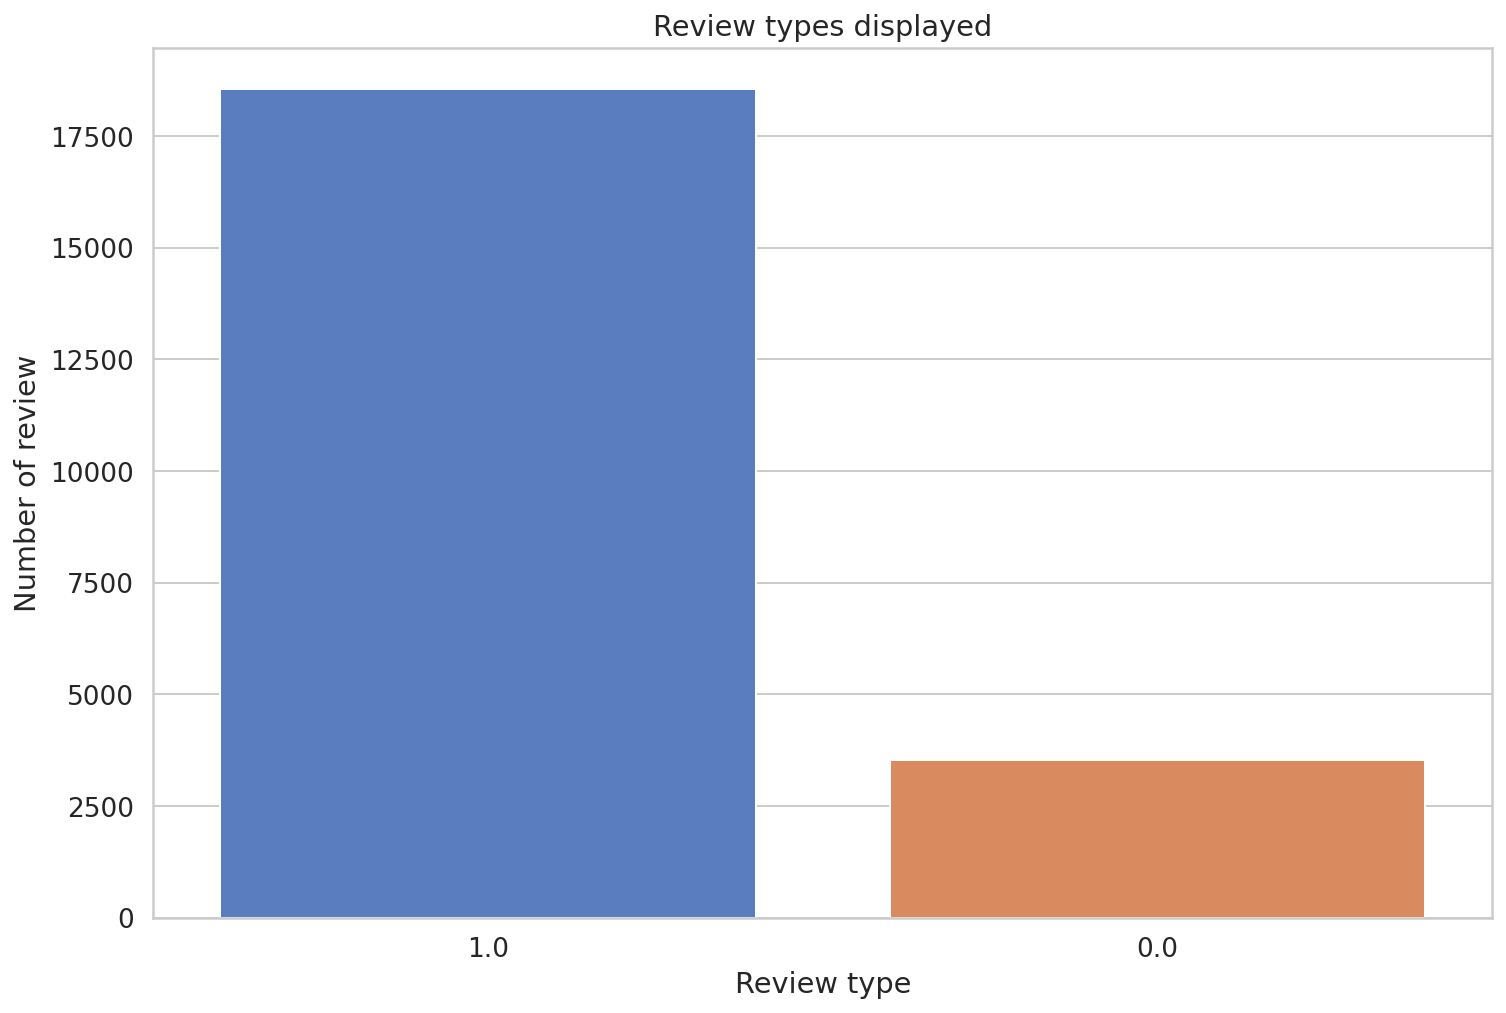
\includegraphics[width=1\textwidth]{images/output_43_1.png}
\caption{Number of ratings per category}
\label{fig:fig_04}
\end{figure}
\FloatBarrier
\subsubsection{Resample reviews}
\label{chap:resample}
In order to be able to train my model later on, I need to have the same amount of test data for each category. For this reason, I should limit the larger category to the value of the smaller one.
The code for this operation:
        \begin{tcolorbox}[breakable, size=fbox, boxrule=1pt, pad at break*=1mm,colback=cellbackground, colframe=cellborder]
\begin{Verbatim}[commandchars=\\\{\},fontsize=\footnotesize]
\PY{c+c1}{\PYZsh{} Get same number of reviews for each type}
\PY{n}{bad\PYZus{}reviews} \PY{o}{=} \PY{n}{film\PYZus{}df\PYZus{}de}\PY{p}{[}\PY{n}{film\PYZus{}df\PYZus{}de}\PY{o}{.}\PY{n}{Positive} \PY{o}{==} \PY{l+m+mi}{0}\PY{p}{]}
\PY{n}{good\PYZus{}reviews} \PY{o}{=} \PY{n}{film\PYZus{}df\PYZus{}de}\PY{p}{[}\PY{n}{film\PYZus{}df\PYZus{}de}\PY{o}{.}\PY{n}{Positive} \PY{o}{==} \PY{l+m+mi}{1}\PY{p}{]}

\PY{n}{sample\PYZus{}len} \PY{o}{=} \PY{n+nb}{len}\PY{p}{(}\PY{n}{bad\PYZus{}reviews}\PY{p}{)}

\PY{n}{bad\PYZus{}df} \PY{o}{=} \PY{n}{bad\PYZus{}reviews}
\PY{n}{good\PYZus{}df} \PY{o}{=} \PY{n}{good\PYZus{}reviews}\PY{o}{.}\PY{n}{sample}\PY{p}{(}\PY{n}{n}\PY{o}{=}\PY{n}{sample\PYZus{}len}\PY{p}{,} \PY{n}{random\PYZus{}state}\PY{o}{=}\PY{n}{RANDOM\PYZus{}SEED}\PY{p}{)}

\PY{n}{film\PYZus{}review\PYZus{}df} \PY{o}{=} \PY{n}{good\PYZus{}df}\PY{o}{.}\PY{n}{append}\PY{p}{(}\PY{n}{bad\PYZus{}df}\PY{p}{)}\PY{o}{.}\PY{n}{reset\PYZus{}index}\PY{p}{(}\PY{n}{drop}\PY{o}{=}\PY{k+kc}{True}\PY{p}{)}
\PY{n}{film\PYZus{}review\PYZus{}df}\PY{o}{.}\PY{n}{shape}
\end{Verbatim}
\end{tcolorbox}

By doing so, the data will have  the same number of entries as in Figure~\ref{fig:fig_05}.

\begin{figure}[H]
\centering
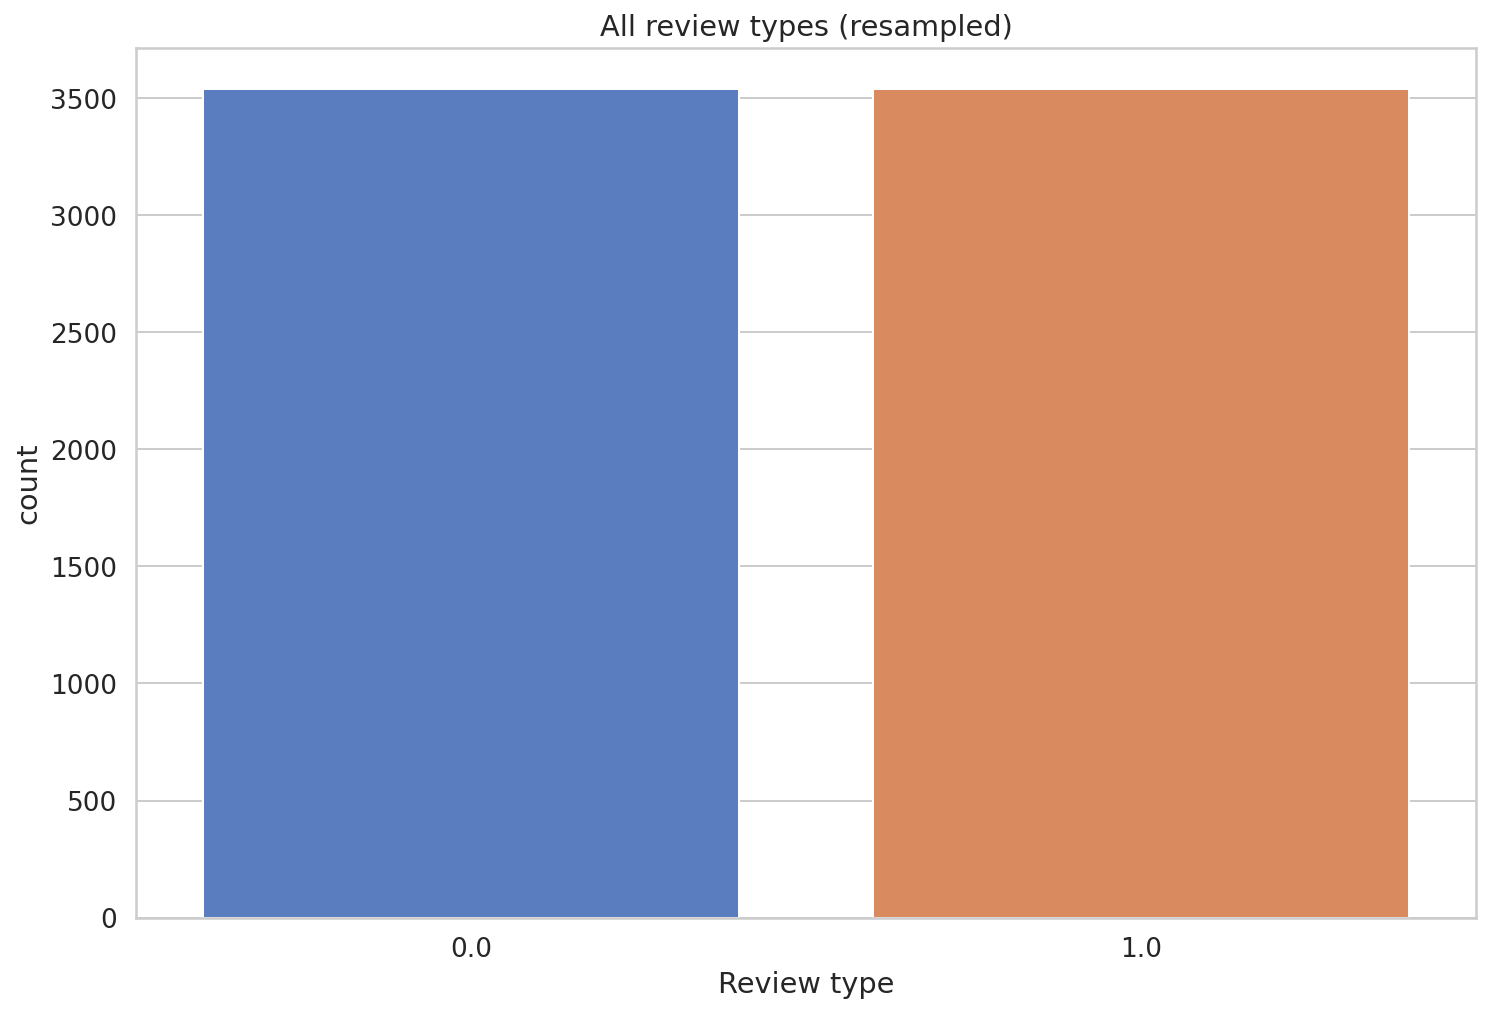
\includegraphics[width=1\textwidth]{images/output_47_0.png}
\caption{Uniform size of the categories}
\label{fig:fig_05}
\end{figure}
\FloatBarrier

\subsubsection{Preprocessing}
In this section I deal with the preparation of the data to give then to the model.
Before I start with splitting the dataset, I randomize the entire dataset by shuffling the data in a totally random way. 
The first thing to do is to split the dataframes I got after cleaning into 3 parts:
\begin{itemize}
    \item train set
    \item validation set
    \item test set
\end{itemize}

Training set is a sample of data used to fit the model, the model trains and learns from this data.\\
Validation set is used to evaluate the trained model. With the evaluation of the model, it is possible to make a fine-tune of the model and to modify the hyperparameters.\\
Test set provides the gold standard used to evaluate the model.\\

Figure~\ref{fig:fig_06} shown an example of the split of a dataset\footnote{Reference figure \url{https://towardsdatascience.com/train-validation-and-test-sets-72cb40cba9e7}}: 
\begin{figure}[H]
\centering
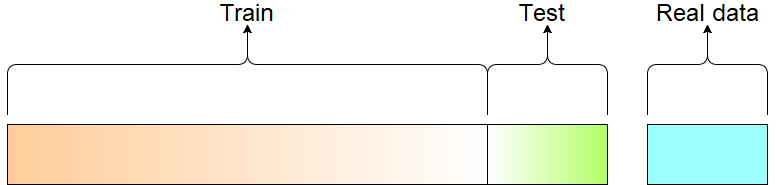
\includegraphics[width=1\textwidth]{images/traintestvali.jpg}
\caption{Data split}
\label{fig:fig_06}
\end{figure}
\FloatBarrier

Thanks to the library sklearn.model\_selection.train\_test\_split I can easily split my dataset in training and test. The division is done with a ratio 80\%(training)/20\%(test)

    \begin{tcolorbox}[breakable, size=fbox, boxrule=1pt, pad at break*=1mm,colback=cellbackground, colframe=cellborder]
\begin{Verbatim}[commandchars=\\\{\},fontsize=\small]
\PY{n}{train}\PY{p}{,} \PY{n}{test} \PY{o}{=} \PY{n}{train\PYZus{}test\PYZus{}split}\PY{p}{(}\PY{n}{film\PYZus{}review\PYZus{}df}\PY{p}{,}\PY{n}{test\PYZus{}size}\PY{o}{=}\PY{l+m+mf}{0.2}\PY{p}{)}
\end{Verbatim}
\end{tcolorbox}

   \begin{Verbatim}[commandchars=\\\{\},fontsize=\small]
size of training set: 5660
size of validation set: 1416
    \end{Verbatim}

Finally, in order to have data that is usable by the Ktrain library, I need to transform both sets into lists, and eliminate rows with null values.
\section{Sentiment Analysis}
This is the main section as far as the project is concerned, in fact here will be treated the sentiment analysis, then first approach, creation of the model and work on the data predicted by the model.
My model can basically be imagined as a function that takes arbitrary text as input, evaluates it, and classifies it into a scale of emotions from negative to positive.
To develop and train a model with this capability requires many prebuilt datasets of real examples from the Internet. These are then used to feed the model so that it can learn from these datasets and deduce correlations. Based on these correlations, the model will then be able to process arbitrary texts and assign sentiment values to them.

\subsection{The first approach to the thesis}
Before I started doing any work on sentiment analysis, I had to do many hours of research.
At the end of the 5th semester, we saw in class how to do text analysis, so with techniques of:
\begin{itemize}
    \item regex,
    \item sentence segmentation (character sequence into sentences), 
    \item tokenization (character sequence into tokens (words)),
    \item stop word elimination (the, a, to, of, etc),
    \item normalization (U.S.A. or USA as no difference),
    \item lemmatization,
    \item stemming,
    \item using NLTK library.
\end{itemize}

So, the first approach was to work with an NLTK library, and do text analysis.
However, doing research I have seen that in recent times another method has become more famous and has become the state of the art in all respects with regard to the task of text classification, text summarisation, question answering and sentiment analysis.
I am talking about BERT.
As I continued in my research I saw not only how famous BERT had become in a short time, but also how much it made machine learning work easier, thanks to BERT Natural Language Processing (NLP) became easy and accessible for everyone.
Becoming so used and famous, it caused in a short time the creation of several libraries and methods related to BERT.
After working on the datasets, the biggest difficulty was finding the version of BERT and related libraries that would best suit them.
For this task, I invested a lot of time and research to figure out which BERT is right for me.
Finally, my choice fell on BERT-base with Hugging Face's Transformes as library.
The convenience of these transformers is that you can use thousands of pre-trained templates for task text classification, information extraction, question answering, etc. in over 100 languages.

\subsection{Ktrain}
\label{chap:Ktrain model}
Now that I am clear on the tools, all I have to do is set up the work.
To be able to do something of my own I thought to work also on the dataset, so with Ktrain I did not use the IMDB dataset, but I opted for the Filmstarts dataset.

Ktrain can be used thanks to two different APIs:
\begin{itemize}
    \item automatic API,
    \item manual API.
\end{itemize}

The automatic API has a limited choice of classifiers (6), having to create a model that works on the German language I need a specific classifier, so I am going to use the manual API because I can use any pre-trained model that you can find at the Hugging Face website \cite{noauthor_hugging_nodate}.
The manual model is an improvement of the automatic model, the part about the automatic model can be found in \autoref{chap:model filmstars auto}.


\paragraph{Process the data}
The data has been cleaned previously as seen in \autoref{chap:work on dataset}, the data then only needs to be tokenized in order to be used.  


\textbf{Token what is?}\cite{noauthor_what_2019}
Tokenization is one of the most common tasks when it comes to working with text data, in a nutshell is the division of a text (sentence, paragraph or a whole text) into individual words . Each word is called a token.
However, BERT cannot use words directly, so there will be a need to encode each token into numbers so that it is usable by the machine.
BERT only digests tokens with a maximum length of 512.
It does not make sense to use the maximum length when the tokens are shorter, so in order to save model work and to speed up preprocessing work I need to find the maximum length of each review.

What I need to do now is figure out the maximum length of each review, taking, I just need to find what is the max\_len I am interested in to create the model:

    \begin{tcolorbox}[breakable, size=fbox, boxrule=1pt, pad at break*=1mm,colback=cellbackground, colframe=cellborder]
\begin{Verbatim}[commandchars=\\\{\},fontsize=\footnotesize]
\PY{n}{textToCheck} \PY{o}{=} \PY{n}{film\PYZus{}review\PYZus{}df}\PY{o}{.}\PY{n}{Review}\PY{p}{[}\PY{l+m+mi}{1}\PY{p}{]}
\end{Verbatim}
\end{tcolorbox}

    \begin{tcolorbox}[breakable, size=fbox, boxrule=1pt, pad at break*=1mm,colback=cellbackground, colframe=cellborder]
\begin{Verbatim}[commandchars=\\\{\},fontsize=\footnotesize]
\PY{k}{for} \PY{n}{txt} \PY{o+ow}{in} \PY{n}{textToCheck}\PY{p}{:}
    \PY{n}{tokens} \PY{o}{=} \PY{n}{tokenizer\PYZus{}hugg}\PY{o}{.}\PY{n}{encode}\PY{p}{(}\PY{n}{txt}\PY{p}{,} \PY{n}{max\PYZus{}length}\PY{o}{=}\PY{l+m+mi}{512}\PY{p}{)}
    \PY{n}{token\PYZus{}lens}\PY{o}{.}\PY{n}{append}\PY{p}{(}\PY{n+nb}{len}\PY{p}{(}\PY{n}{tokens}\PY{p}{)}\PY{p}{)}
\end{Verbatim}
\end{tcolorbox}

\begin{figure}[ht!]
\centering
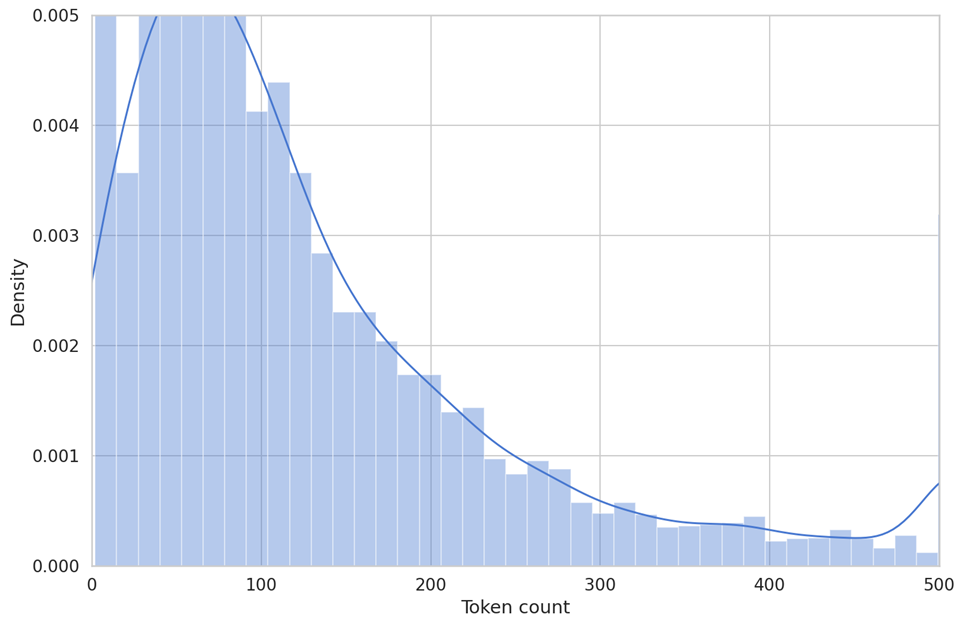
\includegraphics[width=1\textwidth]{images/512.png}
\caption{Ktrain learner plot}
\label{fig:fig_07}
\end{figure}
\FloatBarrier

From Figure~\ref{fig:fig_07} it is possible to see that after 400 tokens the density is less than 0.001. For this reason I can set max len to 400.

\subsubsection{Build a Model and Wrap in Learner}
\label{chap:ktrain build a model}
In this section is described, the construction of the model using the ktrain library.

\paragraph{Model}
For this project, I looked for a pre-trained model that would be ideal. My choice fell on dbmz/bert-german-cased.
This is one of the best models I found on Hugging Face \cite{noauthor_dbmdzbert-base-german-uncased_nodate}, from the site it is possible to read that:
\begin{quote}
    The source data for the model consists of a recent Wikipedia dump, EU Bookshop corpus, Open Subtitles, CommonCrawl, ParaCrawl and News Crawl. This results in a dataset with a size of 16GB and 2,350,234,427 tokens.
\end{quote}

As the git name suggests dbmz \cite{noauthor_open_nodate} is a Open Source at the Bayerische Staatsbibliothek from the MDZ Digital Library team at the Bavarian State Library \cite{noauthor_munich_nodate} based in Munich. Dbmz is one of the leading exponents of the German language and more.

In order to work with Ktrain, I then had to set the model's name:

 \begin{tcolorbox}[breakable, size=fbox, boxrule=1pt, pad at break*=1mm,colback=cellbackground, colframe=cellborder]
\begin{Verbatim}[commandchars=\\\{\},fontsize=\footnotesize]
\PY{n}{MODEL\PYZus{}NAME} \PY{o}{=} \PY{l+s+s1}{\PYZsq{}}\PY{l+s+s1}{dbmdz/bert\PYZhy{}base\PYZhy{}german\PYZhy{}cased}\PY{l+s+s1}{\PYZsq{}}
\end{Verbatim}
\end{tcolorbox}

From the Ktrain documentation it is possible to understand how to use the library.
The text.Transformer() function allows me to do text classification using a Hugging Face transformers.

    \begin{tcolorbox}[breakable, size=fbox, boxrule=1pt, pad at break*=1mm,colback=cellbackground, colframe=cellborder]
\begin{Verbatim}[commandchars=\\\{\},fontsize=\footnotesize]
\PY{n}{t} \PY{o}{=} \PY{n}{text}\PY{o}{.}\PY{n}{Transformer}\PY{p}{(}\PY{n}{MODEL\PYZus{}NAME}\PY{p}{,} \PY{n}{maxlen}\PY{o}{=}\PY{l+m+mi}{400}\PY{p}{,} \PY{n}{class\PYZus{}names}\PY{o}{=}\PY{p}{[}\PY{l+s+s1}{\PYZsq{}}\PY{l+s+s1}{0}\PY{l+s+s1}{\PYZsq{}}\PY{p}{,}\PY{l+s+s1}{\PYZsq{}}\PY{l+s+s1}{1}\PY{l+s+s1}{\PYZsq{}}\PY{p}{]}\PY{p}{)}
\end{Verbatim}
\end{tcolorbox}

The t.preprocess() function allows me to use the transformer to tokenize and encode the train and test datasets.
    \begin{tcolorbox}[breakable, size=fbox, boxrule=1pt, pad at break*=1mm,colback=cellbackground, colframe=cellborder]
\begin{Verbatim}[commandchars=\\\{\},fontsize=\footnotesize]
\PY{n}{trn} \PY{o}{=} \PY{n}{t}\PY{o}{.}\PY{n}{preprocess\PYZus{}train}\PY{p}{(}\PY{n}{xtrain\PYZus{}list}\PY{p}{,}\PY{n}{ytrain\PYZus{}list}\PY{p}{)}
\end{Verbatim}
\end{tcolorbox}

    \begin{Verbatim}[commandchars=\\\{\},fontsize=\footnotesize]
preprocessing train{\ldots}
language: de
train sequence lengths:
        mean : 105
        95percentile : 317
        99percentile : 623
    \end{Verbatim}

    \begin{Verbatim}[commandchars=\\\{\},fontsize=\footnotesize]
Is Multi-Label? False
    \end{Verbatim}

    \begin{tcolorbox}[breakable, size=fbox, boxrule=1pt, pad at break*=1mm,colback=cellbackground, colframe=cellborder]
\begin{Verbatim}[commandchars=\\\{\},fontsize=\footnotesize]
\PY{n}{val} \PY{o}{=} \PY{n}{t}\PY{o}{.}\PY{n}{preprocess\PYZus{}test}\PY{p}{(}\PY{n}{xtest\PYZus{}list}\PY{p}{,} \PY{n}{ytest\PYZus{}list}\PY{p}{)}
\end{Verbatim}
\end{tcolorbox}

    \begin{Verbatim}[commandchars=\\\{\},fontsize=\footnotesize]
preprocessing test{\ldots}
language: de
test sequence lengths:
        mean : 111
        95percentile : 342
        99percentile : 619
    \end{Verbatim}
    
My model is nothing more than a wrap of all the previous steps, added to the get\_classifier() function:  
    \begin{tcolorbox}[breakable, size=fbox, boxrule=1pt, pad at break*=1mm,colback=cellbackground, colframe=cellborder]
\begin{Verbatim}[commandchars=\\\{\},fontsize=\footnotesize]
\PY{n}{model} \PY{o}{=} \PY{n}{t}\PY{o}{.}\PY{n}{get\PYZus{}classifier}\PY{p}{(}\PY{p}{)}
\end{Verbatim}
\end{tcolorbox}


\paragraph{get\_learner}
Now that I have a model, I can create a learner. A learner object will be used to help tune and train my network.
    \begin{tcolorbox}[breakable, size=fbox, boxrule=1pt, pad at break*=1mm,colback=cellbackground, colframe=cellborder]
\begin{Verbatim}[commandchars=\\\{\},fontsize=\footnotesize]
\PY{n}{learner} \PY{o}{=} \PY{n}{ktrain}\PY{o}{.}\PY{n}{get\PYZus{}learner}\PY{p}{(}\PY{n}{model}\PY{p}{,} \PY{n}{train\PYZus{}data}\PY{o}{=}\PY{n}{trn}\PY{p}{,} \PY{n}{val\PYZus{}data}\PY{o}{=}\PY{n}{val}\PY{p}{,} \PY{n}{batch\PYZus{}size}\PY{o}{=}\PY{l+m+mi}{12}\PY{p}{)}
\end{Verbatim}
\end{tcolorbox}
\subsubsection{Model training}
\label{chap:model training}
\paragraph{learner.lr\_find and plot()}
With a learner object, I can simulate a workout on different learning rates, so I can see the best one, I will use the function:
    \begin{tcolorbox}[breakable, size=fbox, boxrule=1pt, pad at break*=1mm,colback=cellbackground, colframe=cellborder]
\begin{Verbatim}[commandchars=\\\{\},fontsize=\footnotesize]
\PY{n}{learner}\PY{o}{.}\PY{n}{lr\PYZus{}find}\PY{p}{(}\PY{p}{)}
\end{Verbatim}
\end{tcolorbox}


With the learner.lr\_plot() function I can plot the graph of what I just trained, so can I visually inspect the loss plot to help identify the maximal learning rate associated with falling loss.
Figure~\ref{fig:fig_08} shows how it works:
 \begin{tcolorbox}[breakable, size=fbox, boxrule=1pt, pad at break*=1mm,colback=cellbackground, colframe=cellborder]
\begin{Verbatim}[commandchars=\\\{\},fontsize=\footnotesize]
\PY{n}{learner}\PY{o}{.}\PY{n}{lr\PYZus{}plot}\PY{p}{(}\PY{p}{)}
\end{Verbatim}
\end{tcolorbox}

\begin{figure}[ht!]
\centering
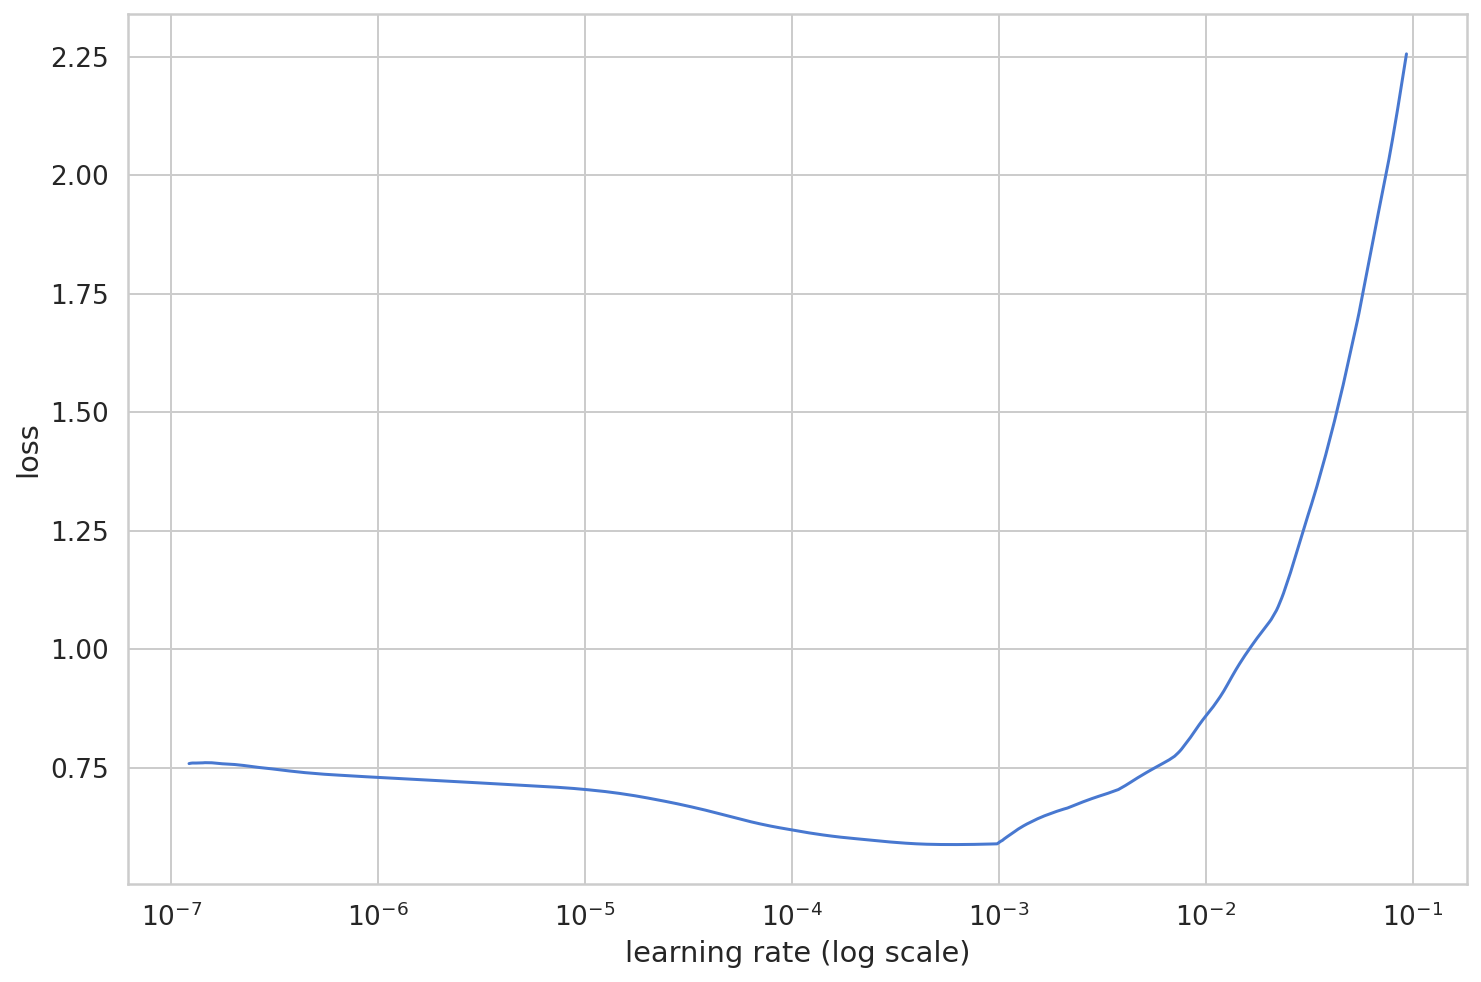
\includegraphics[width=1\textwidth]{images/output_118_1.png}
\caption{Ktrain learner plot}
\label{fig:fig_08}
\end{figure}
\FloatBarrier

\paragraph{autofit}
Now I am going to use the autofit \cite{noauthor_amaiyaktrainautofit_nodate} method to train the model with the parameters I found earlier.
The autofit method use a cyclical learning rate schedule. The default learning rate is the triangular learning rate policy \cite{smith_cyclical_2017}.
As before, I invoked the help function to better understand how the autofit function works.
The autofit method accepts two primary arguments, learning rate and epochs.
If epochs are not defined then the method will train until the validation loss no longer improves after a certain period. This period is also configurable using the early\_stopping argument. 

I used also another two argument, reduce\_on\_plateau and checkpoint\_folder.\\
reduce\_on\_plateau check if the validation loss fails to improve after a specified number of epochs.
checkpoint\_folder folder path in which to save the model weights for each epoch.\\
Next, I called the function as below:
    \begin{tcolorbox}[breakable, size=fbox, boxrule=1pt, pad at break*=1mm,colback=cellbackground, colframe=cellborder]
\begin{Verbatim}[commandchars=\\\{\},fontsize=\footnotesize]
\PY{n}{learner}\PY{o}{.}\PY{n}{autofit}\PY{p}{(}\PY{l+m+mf}{3e\PYZhy{}5}\PY{p}{,} \PY{n}{reduce\PYZus{}on\PYZus{}plateau}\PY{o}{=}\PY{l+m+mi}{3}\PY{p}{,} \PY{n}{checkpoint\PYZus{}folder}\PY{o}{=}\PY{l+s+s1}{\PYZsq{}}\PY{l+s+s1}{./checkpointNewModel25.04/}\PY{l+s+s1}{\PYZsq{}}\PY{p}{)}
\end{Verbatim}
\end{tcolorbox}


  \begin{Verbatim}[commandchars=\\\{\},fontsize=\footnotesize]
early\_stopping automatically enabled at patience=5


begin training using triangular learning rate policy with max lr of 3e-05{\ldots}
Epoch 1/1024
472/472 [==============================] - 190s 378ms/step - loss: 0.4936 -
accuracy: 0.7200 - val\_loss: 0.1846 - val\_accuracy: 0.9300
Epoch 2/1024
472/472 [==============================] - 178s 375ms/step - loss: 0.1627 -
accuracy: 0.9432 - val\_loss: 0.1748 - val\_accuracy: 0.9350
...
...
Epoch 00005: Reducing Max LR on Plateau: new max lr will be 1.5e-05 (if not
early\_stopping).
Epoch 6/1024
472/472 [==============================] - 178s 376ms/step - loss: 0.0299 -
accuracy: 0.9921 - val\_loss: 0.2663 - val\_accuracy: 0.9307
Epoch 7/1024
472/472 [==============================] - 179s 376ms/step - loss: 0.0178 -
accuracy: 0.9949 - val\_loss: 0.2605 - val\_accuracy: 0.9314
Restoring model weights from the end of the best epoch.
Epoch 00007: early stopping
Weights from best epoch have been loaded into model.
    \end{Verbatim}
    
\subsubsection{Results}
\paragraph{validate}
Using the:
    \begin{tcolorbox}[breakable, size=fbox, boxrule=1pt, pad at break*=1mm,colback=cellbackground, colframe=cellborder]
\begin{Verbatim}[commandchars=\\\{\},fontsize=\footnotesize]
\PY{n}{learner}\PY{o}{.}\PY{n}{validate}\PY{p}{(}\PY{p}{)}
\end{Verbatim}
\end{tcolorbox}method I can create a confusion matrix on the newly trained data in order to get a more detailed picture:
    \begin{Verbatim}[commandchars=\\\{\},fontsize=\footnotesize]
              precision    recall  f1-score   support

           0       0.94      0.93      0.94       725
           1       0.93      0.94      0.93       690

    accuracy                           0.93      1415
   macro avg       0.93      0.94      0.93      1415
weighted avg       0.94      0.93      0.93      1415

    \end{Verbatim}
            \begin{tcolorbox}[breakable, size=fbox, boxrule=.5pt, pad at break*=1mm, opacityfill=0]
\begin{Verbatim}[commandchars=\\\{\},fontsize=\footnotesize]
array([[14883,  2497],
       [ 2610, 14915]])
\end{Verbatim}
\end{tcolorbox}


\textbf{What is a confusion matrix?}

Confusion matrix is one of the easiest and most intuitive metrics to check the accuracy of a model.
It is mostly used for classification problems, as in my example.

The confusion matrix is calculated as shown in Figure~\ref{fig:fig_cm}:
\begin{figure}[ht!]
\centering
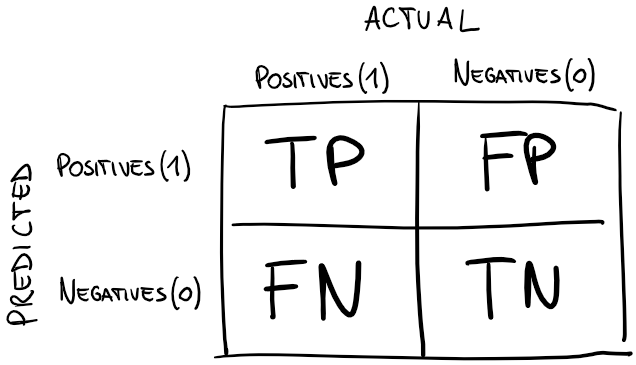
\includegraphics[width=0.5\textwidth]{images/cm.png}
\caption{Confusion matrix}
\label{fig:fig_cm}
\end{figure}
\FloatBarrier
In my case I have the two classes 0 (negative) and 1 (positive).

\textbf{True Positive(TP)}: number of cases in which the value of the real data is 1 (positive) and the prediction of the model is also 1. Correct prediction.

\textbf{True Negative(TN)}: number of the real cases is 0 (negative) and the cases predicted from the model are 0. Correct prediction.

\textbf{False Positive(FP)}: number of the real cases are 0 (negative) and the cases predicted from the model are 1 (positive). Wrong prediction. 

\textbf{False Negative(FN)}: number of the real cases are 1 (positive) and the cases predicted from the model are 0 (negative). Wrong prediction. 

Thanks to the confusion matrix, several factors can be calculated:
\begin{itemize}
    \item accuracy
    \item precision
    \item recall or sensitivity
    \item f1 score.
\end{itemize}

\textbf{Accuracy} \cite{brownlee_how_2020}:\\
This metric, when talking about tasks such as classification, is the number of correct predictions made by the model, out of all the predictions made.
Figure~\ref{fig:fig_acc} shows how this metric is calculated:
\begin{figure}[ht!]
\centering
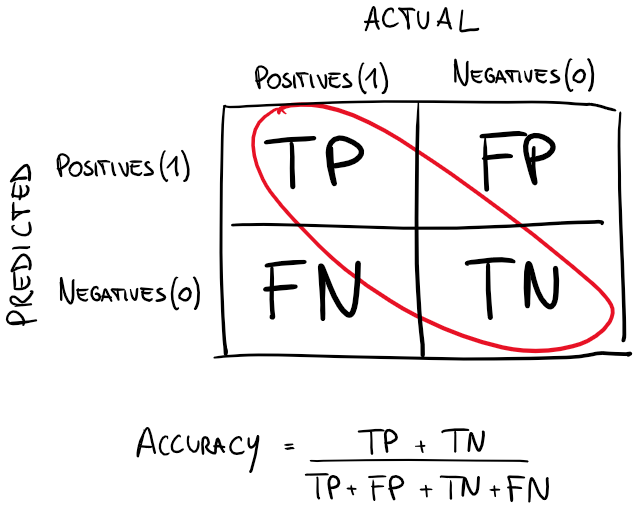
\includegraphics[width=0.5\textwidth]{images/acc.png}
\caption{Accuracy}
\label{fig:fig_acc}
\end{figure}
\FloatBarrier

Accuracy is a good measure when the classes of targets in the data are nearly balanced. 
example class A= 60\% and class B= 40\%. 
If instead I have a big difference like, class A = 85\% and class B=15\% the accuracy cannot be used because it is not a reliable value.

For this reason I made a resample of my dataset, to have small difference between the two classes. See \ref{chap:resample}.

In my case I have a great accuracy (93\%) counting that the model is based on a language where punctuation, Cased or Uncased has a great influence, I can be satisfied.


\textbf{Precision} \cite{brownlee_how_2020}:\\
Precision is the ratio of correctly predicted positive observations to the total predicted positive observations. 
The question that this metric answers is: 
of all the articles labelled as positive, how many of them are actually positive?

High precision relates to the low false positive (FP) rate. 
Figure~\ref{fig:fig_pre} shows how this metric is calculated:
\begin{figure}[ht!]
\centering
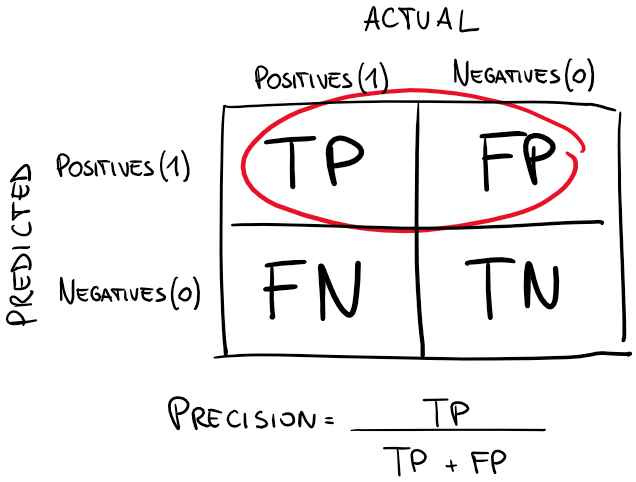
\includegraphics[width=0.5\textwidth]{images/prec.png}
\caption{Precision}
\label{fig:fig_pre}
\end{figure}
\FloatBarrier

Precision is used in cases where we need to be certain, so it is not the quantity that matters but the quality. For example, if I must make a prediction about cancer cases, I must be 100\% sure that it is correct even if it is only one case.
In my case it is better to have great accuracy, but if I have mistaken, I do not have repercussions like for example in the medical field.

In my case Precision (0 = 94\%, 1 = 93\%) is aligned with all other values.

\textbf{Recall (or Sensitivity)} \cite{brownlee_how_2020}:\\
Recall is the ratio of correctly predicted positive observations to all observations in actual class. Answers the question:
of all the articles that are truly positive, how many of them were predicted correctly? 
Figure~\ref{fig:fig_rec} shows how this metric is calculated:
\begin{figure}[ht!]
\centering
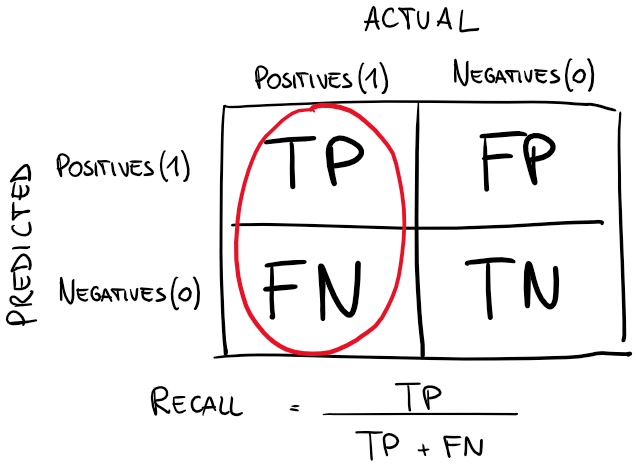
\includegraphics[width=0.5\textwidth]{images/rec.png}
\caption{Recall/Sensitivity}
\label{fig:fig_rec}
\end{figure}
\FloatBarrier

Recall is used not so much to figure out which cases were predicted correctly, but more the capture of all "positive sentiment" cases with the answer as "positive".

In my case Recall (0 = 93\%, 1 = 94\%) is aligned with all other values.

\textbf{F1 score} \cite{brownlee_how_2020}:\\
We need a metric that takes Precision and Recall into account, that's why F1 score exists.
F1 Score is the weighted average of Precision and Recall.
Figure~\ref{fig:fig_f1} shows how this metric is calculated:
\begin{figure}[ht!]
\centering
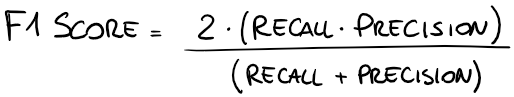
\includegraphics[width=0.4\textwidth]{images/f1.png}
\caption{F1 score}
\label{fig:fig_f1}
\end{figure}
\FloatBarrier

F1 is usually more useful than accuracy, especially if we have an uneven class distribution. Accuracy works best if false positives and false negatives have similar cost. If the cost of false positives and false negatives are very different, it is better to look at both Precision and Recall.

In my case F1 score (0 = 94\%, 1 = 93\%) is aligned with all other values.


\subsubsection{Save and reload model}
Thanks to the last update of Ktrain in March, to save the trained model and its weights I will simply use:
    \begin{tcolorbox}[breakable, size=fbox, boxrule=1pt, pad at break*=1mm,colback=cellbackground, colframe=cellborder]
\begin{Verbatim}[commandchars=\\\{\},fontsize=\footnotesize]
\PY{n}{predictor}\PY{o}{.}\PY{n}{save}\PY{p}{(}\PY{l+s+s1}{\PYZsq{}}\PY{l+s+s1}{./modelsave/bertDe\PYZus{}predictor\PYZus{}93}\PY{l+s+s1}{\PYZsq{}}\PY{p}{)}
\end{Verbatim}
\end{tcolorbox}

Even simpler is to load a model, in fact used the function load\_predictor() by specifying from which path to take the model, I can already in the next line make predictions.
\begin{tcolorbox}[breakable, size=fbox, boxrule=1pt, pad at break*=1mm,colback=cellbackground, colframe=cellborder]
\begin{Verbatim}[commandchars=\\\{\},fontsize=\footnotesize]
\PY{c+c1}{\PYZsh{} reload predictor}
\PY{n}{predictor} \PY{o}{=} \PY{n}{ktrain}\PY{o}{.}\PY{n}{load\PYZus{}predictor}\PY{p}{(}\PY{l+s+s1}{\PYZsq{}}\PY{l+s+s1}{./modelsave/bertDe\PYZus{}predictor\PYZus{}93}\PY{l+s+s1}{\PYZsq{}}\PY{p}{)}
\PY{n}{predictor}\PY{o}{.}\PY{n}{predict}\PY{p}{(}\PY{l+s+s1}{\PYZsq{}}\PY{l+s+s1}{Heute ist ein schöner Tag.}\PY{l+s+s1}{\PYZsq{}}\PY{p}{)}
\end{Verbatim}
\end{tcolorbox}


\subsection{Newspaper API's}
\label{chap:news apis}
Now that I have a trained and working model, what I am missing is data from Swiss newspapers.
To do this I used some Application Programming Interfaces (API):
\begin{itemize}
    \item NewsAPI \cite{noauthor_news_nodate}
    \item GNewsAPI \cite{noauthor_gnews_nodate}
\end{itemize}

I have used both APIs in developer mode for free.

NewsAPI allows me to:
\begin{itemize}
    \item search all articles and get live top headlines,
    \item new articles available with 1 hour delay,
    \item search articles up to a month old,
    \item 100 requests per day,
    \item No extra requests available,
    \item No uptime SLA,
    \item Basic support.
\end{itemize}

GnewAPI allows me to:
\begin{itemize}
    \item 100 requests per day,
    \item basic support,
    \item up to 10 articles returned per request,
    \item maximum of 1 request per second.
\end{itemize}
The main idea was to use the API in a python file, so that I have the news of the day every time I launch the file.
I used two APIs because I have limitations on the number of requests per day and the number of items per request.
To avoid these limitations I imported both APIs in a single python file, for each API I made a request per category and saved the response in json.
Categories are:
\begin{itemize}
    \item world,
    \item nation,
    \item business,
    \item technology,
    \item entertainment,
    \item sports,
    \item science,
    \item health.
\end{itemize}

I transformed the jsons into dataframes, for each dataframe I checked to make sure they were not empty and deleted the columns I did not need.
I noticed that NewsAPI returns only newspapers in German language even if I change the settings.

Once I have the different clean dataframes I put them in a list and merge them into one dataframe thanks to the pandas concat() function.
In the list then I check that there are no duplicates, and if there are I delete them, always thanks to pandas with the drop\_duplicates() function.

By doing so I expect to have about 30 articles in German for each category.

At this point still using pandas to\_csv, I export and save the dataframe in csv format with its timestamp.

In order to have more freedom I export not only the concatenated dataframe, but also each individual dataframe category.

Now that I have a working python script what I need is just to make it automatic in order to make one request per day.
Using the virtual machine always active, I created, thanks to the windows task scheduler, a task that would start my script once a day and save the files in a certain folder.

\subsection{Model test with Newspaper data}
\label{chap:model test newspaper}
\subsubsection{Ground truth}
After a few days of scraping data thanks to my script, I decided to do some tests with the model I had trained. 
First, I imported the data into my environment, then thanks to pandas I started to analyze it and then I made the predictions.
The dataset I imported has the following columns:
\begin{itemize}
    \item source
    \item title
    \item description
\end{itemize}

Before I can look at the model results, I need to create a ground truth.
In the data science world, it is called "ground truth" when I compare a result created by a user "by hand" with what the model predicted.
This is to be able to compare the real data with the data from the model. 
So, I took a sample of a dataset, and hand classified a positive or negative sentiment for each newspaper article.
I started by ranking the sentiment at the description of each article without reading the title first, and then did the same at the title, independent of the description. I did this because some descriptions without reading the title were of one sentiment, but with title attached were of the opposite sentiment.
One problem with sentiment prediction I had when the article was "a fact". Normally it can be interpreted as neutral. In that case it can be both, I kept right whether the model predicted positive or negative.

Once I have a ground truth, I tested the model and had it make predictions on the description column, and then on the title column.

These were the results:

\begin{longtable}[c]{|l|l|l|l|}
\hline
\textbf{Model} & \textbf{Accuracy} & \textbf{Target} & \textbf{Score} \\ \hline
\endfirsthead
%
\multicolumn{4}{c}%
{{\bfseries Table \thetable\ continued from previous page}} \\
\hline
\textbf{Model} & \textbf{Accuracy} & \textbf{Target} & \textbf{Score} \\ \hline
\endhead
%
Ktrain   Automatic & 90\% & description & 22/30 \\ \hline
Ktrain   Manual & 93\% & description & 26/30 \\ \hline
Ktrain Manual & 93\% & title & 29/30 \\ \hline
\caption{Model comparison}
\label{tab:table-model}\\
\end{longtable}

\subsubsection{Interesting Case Studies}
In Figure~\ref{fig:fig_09} it is possible to see the comparison between the models: 
\begin{figure}[H]
\centering
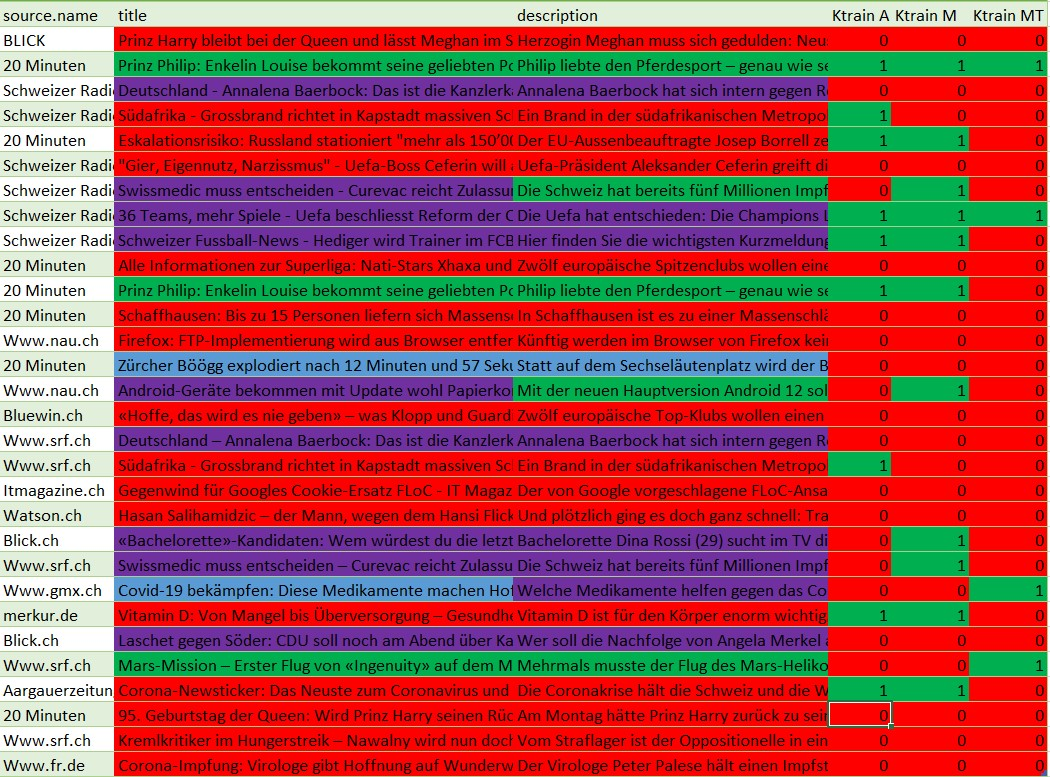
\includegraphics[width=1\textwidth]{images/ktrainmanual.jpg}
\caption{Model Comparison}
\label{fig:fig_09}
\end{figure}
\FloatBarrier
The red and green colors refer to negative(0) or positive(1), purple instead are the neutral cases where a sentiment cannot be defined, so both values from the model I considered them correct.
In blue are in interesting cases, because the text without a context comes across as negative, in fact it is not.

\paragraph{Example:}
"Statt auf dem Sechseläutenplatz wird der Böögg dieses Jahr im Kanton Uri verbrannt. Der Wind sorgte dafür, dass der Kopf schnell explodierte. Der Sommer kann kommen!"

The model classifies this sentence negative for obvious reasons:
something is burned, head exploded, I personally had to inform myself because even I without context was not sure how to classify this news. This shows that the machine is not perfect and cannot understand shades that are difficult even to humans.

\subsubsection{Find the bug}
What can be seen is that the description alone is often predicted positively compared to the title which is predicted negatively.
For this reason the next test sees the Ktrain Manual model doing prediction on "title+description" together, to see if the results improve.

The accuracy of this prediction improved considerably, although I often encountered trivial errors.
So what I did was to use predictor.explain() so I could better understand how the model works and I did several tests.

With predictor.explain() I can generate a visualization.
The visualization technique is called "Explain like I’m 5" (ELI5)\cite{noauthor_textexplainer_nodate} and use the Local Interpretable Model-agnostic Explanations (LIME) algorithm \cite{ribeiro_why_2016}\cite{ribeiro_marcotcrlime_2021}, in which the importance of each single word can be seen based on the final prediction, using an interpretable linear model.
The green words are inferred as contributing to the classification. The red (or pink) words detract from our final prediction. (Shade of color denotes the strength or size of the coefficients in the inferred linear model.)

I created a dataset on purpose with the newspaper header with more data, to be able to make a good comparison.
So, I chose "20 Minuten" to be able to do some tests.

This dataframe has on both "title+description" and "description" 26 negative predictions and 13 positive predictions, while on "title" it has 33 negatives and 6 positives, perfect for understanding what is going on.

Since on both "title+description" and "description" the results match, I focus on the "title" column.

Looking in the dataframe it can be seen that NewsAPI adds at the end of the headline "- newspaper name".

Before effecting the tests there are from explaining some data that help me to understand better how the model works.
\begin{itemize}
    \item \textbf{y=} refers to how the text has been classified, it can be 0 (negative) or 1 (positive),
    \item \textbf{score} is the score that the sentence has obtained looking at the Feature contribution. If the score is negative then y=0 if positive y=1. Higher is the score, higher is the probability value.
    \item \textbf{Contribution} = (weight * feature value) is calculated for each value. For feature values we can have 2 types of feature:
    \begin{itemize}
        \item \textbf{Highlighted in text(sum)},
        \item \textbf{<BIAS>}
    \end{itemize}
    Both of these values can be positive or negative, green or red.
    "Highlighted in text(sum)" indicates the correct feature, while "BIAS" incorrect. These two values are summed together, they can have the same or opposite sign.
\end{itemize}

I did 4 ests on the same sentence with positive ground truth:
\begin{enumerate}
  \item Title with source at the end = \textbf{negative 0.632}
  \begin{figure}[H]
\centering
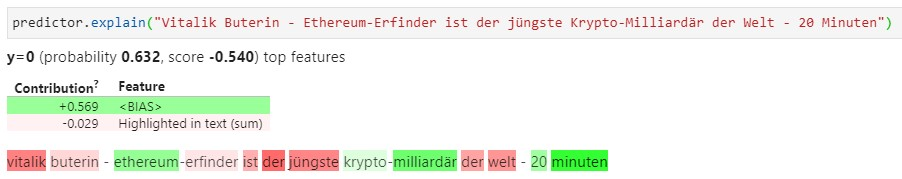
\includegraphics[width=1\textwidth]{images/1text.jpg}
\caption{predictor.explain() test 1}
\label{fig:fig_001}
\end{figure}
\FloatBarrier
The model classifies it as negative, why?
BIAS = +0.569, (incorrect)\\
Highlighted in text(sum) = -0.029, (correct)\\
Score will then be = 0.029 - 0.569 = -0.540.\\
Having negative score, y = 0 with probability = 0.632.

  \item Title without source at the end = \textbf{positive 0.583}
    \begin{figure}[H]
\centering
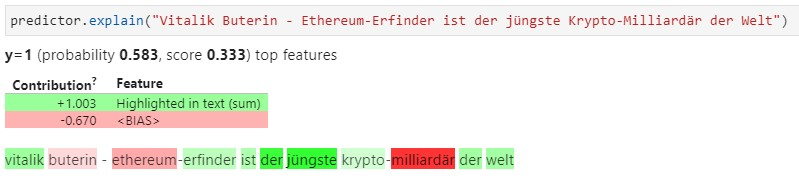
\includegraphics[width=1\textwidth]{images/3text.jpg}
\caption{predictor.explain() test 2}
\label{fig:fig_002}
\end{figure}
\FloatBarrier
Highlighted in text(sum) = +1.003, (correct)\\
BIAS = -0.670, (incorrect)\\
Score will then be = 1.003 - 0.670 = 0.333.\\
Having positive score, y = 1 with probability = 0.583.

\textit{I tried adding punctuation:}
  \item Title with source at the end and no dot = \textbf{positive 0.617}
      \begin{figure}[H]
\centering
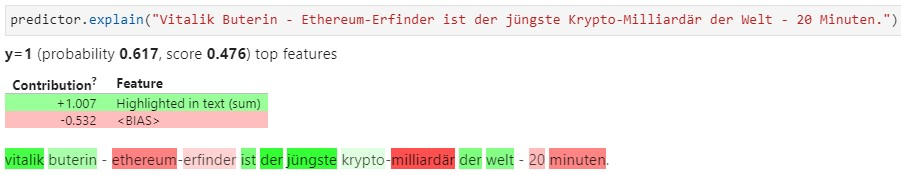
\includegraphics[width=1\textwidth]{images/2text.jpg}
\caption{predictor.explain() test 3}
\label{fig:fig_003}
\end{figure}
\FloatBarrier
Highlighted in text(sum) = +1.007, (correct)\\
BIAS = -0.532, (incorrect)\\
Score will then be = 1.007 - 0.532 = 0.476.\\
Having positive score, y = 1 with probability = 0.617.
  \item Title without source at the end with dot = \textbf{positive 0.849}
      \begin{figure}[H]
\centering
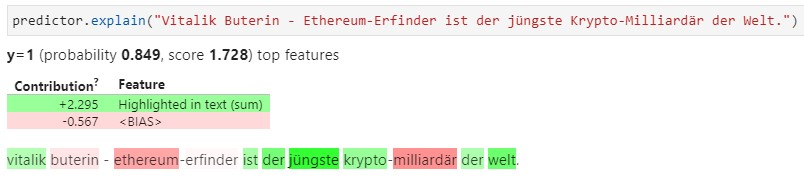
\includegraphics[width=1\textwidth]{images/4text.jpg}
\caption{predictor.explain() test 4}
\label{fig:fig_004}
\end{figure}
\FloatBarrier
Highlighted in text(sum) = +2.295, (correct)\\
BIAS = -0.567, (incorrect)\\
Score will then be = 2.295 - 0.567 = 1.728.\\
Having positive score, y = 1 with probability = 0.849.
\end{enumerate}

It can be understood that punctuation is very important to be able to make predictions correctly, the source already changes the meaning, but the punctuation is at the base.

I then wanted to try "title+description" with what I found previously so:
\begin{enumerate}
    \item "title+description" with “- source” with dot = \textbf{negative 0.641}
        \begin{figure}[H]
\centering
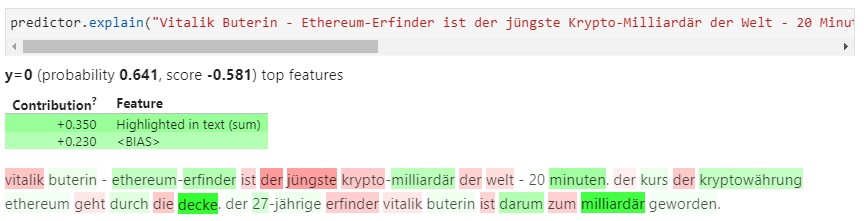
\includegraphics[width=1\textwidth]{images/5text.jpg}
\caption{predictor.explain() "title+description" with source}
\label{fig:fig_005}
\end{figure}
\FloatBarrier
In this case both BIAS and (sum) have the same sign, it means that "Highlighted in text(sum)" goes in the same direction as BIAS, so it is incorrect.
Highlighted in text(sum) = +0.230, (incorrect)\\
BIAS = +0.350, (incorrect)\\
Score will then be = -0.230 - 0.350 = -0.581.\\
Having negative score, y = 0 with probability = 0.641.
    \item "title+description" without “- source” with dot = \textbf{positive 0.578}
        \begin{figure}[H]
\centering
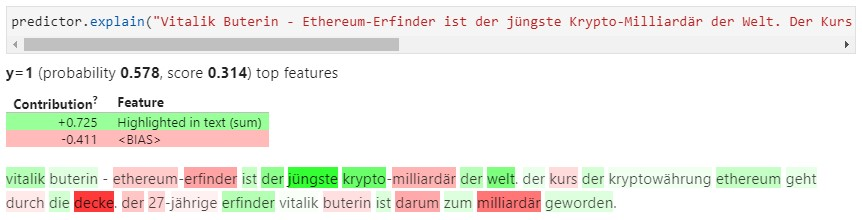
\includegraphics[width=1\textwidth]{images/6text.jpg}
\caption{predictor.explain() "title+description" without source}
\label{fig:fig_006}
\end{figure}
\FloatBarrier
Highlighted in text(sum) = +0.725, (correct)\\
BIAS = -0.411, (incorrect)\\
Score will then be = 0.725 - 0.411 = 0.314.\\
Having positive score, y = 1 with probability = 0.578.
\end{enumerate}

\textbf{Result:} Sentence with punctuation totally changes how the sentiment is predicted, while sentence without source increases the accuracy of the predicted result.

\subsubsection{Fix the bug}
Found this "bug" there is only to understand how to proceed.
The best solution is to clean the data at the root, since NewsAPI gives me unsuitable data, I have two alternatives:
\begin{enumerate}
    \item do not use NewsAPI,
    \item try to solve the problem on data import.
\end{enumerate}

Although the first alternative is the fastest and most immediate, I opted for the second to have a good amount of data on which to make analysis.

I modified the python script to do data scarping\footnote{link git "gnews.py"}.
From the previous version I added having different categories and the timestamp of each article.
Next, I created a python dictionary, filled with all the sources of the various newspapers, so you can clean from each title its source, if the source is not in the dictionary then a warning will notify it.
The code to do this:
\begin{tcolorbox}[breakable, size=fbox, boxrule=1pt, pad at break*=1mm,colback=cellbackground, colframe=cellborder]
\begin{Verbatim}[commandchars=\\\{\},fontsize=\footnotesize]
\PY{k}{def} \PY{n+nf}{cleanup\PYZus{}title}\PY{p}{(}\PY{n}{source}\PY{p}{,} \PY{n}{title}\PY{p}{)}\PY{p}{:}
    \PY{k}{if} \PY{n}{source} \PY{o+ow}{not} \PY{o+ow}{in} \PY{n}{SOURCES}\PY{p}{:}
        \PY{n}{logging}\PY{o}{.}\PY{n}{warn}\PY{p}{(}\PY{l+s+s2}{\PYZdq{}}\PY{l+s+s2}{Unknown source }\PY{l+s+si}{\PYZpc{}s}\PY{l+s+s2}{, leaving as\PYZhy{}is}\PY{l+s+s2}{\PYZdq{}}\PY{p}{,} \PY{n}{source}\PY{p}{)}
        \PY{n+nb}{print}\PY{p}{(}\PY{l+s+s2}{\PYZdq{}}\PY{l+s+s2}{\PYZsq{}}\PY{l+s+s2}{\PYZdq{}}\PY{o}{+}\PY{n}{source}\PY{o}{+}\PY{l+s+s2}{\PYZdq{}}\PY{l+s+s2}{\PYZsq{}}\PY{l+s+s2}{: postfix\PYZus{}title,}\PY{l+s+s2}{\PYZdq{}}\PY{p}{)}
    \PY{k}{return} \PY{n}{SOURCES}\PY{o}{.}\PY{n}{get}\PY{p}{(}\PY{n}{source}\PY{p}{,} \PY{n}{noop}\PY{p}{)}\PY{p}{(}\PY{n}{title}\PY{p}{)}
\end{Verbatim}
\end{tcolorbox}

    \begin{tcolorbox}[breakable, size=fbox, boxrule=1pt, pad at break*=1mm,colback=cellbackground, colframe=cellborder]
\begin{Verbatim}[commandchars=\\\{\},fontsize=\footnotesize]
\PY{k}{def} \PY{n+nf}{clean\PYZus{}dataframe}\PY{p}{(}\PY{n}{df}\PY{p}{)}\PY{p}{:}
    \PY{c+c1}{\PYZsh{} clean title from \PYZsq{}\PYZhy{} newspaper Name\PYZsq{}}
    \PY{n}{title\PYZus{}apply} \PY{o}{=} \PY{n}{df}\PY{o}{.}\PY{n}{apply}\PY{p}{(}
        \PY{k}{lambda} \PY{n}{row} \PY{p}{:} \PY{n}{cleanup\PYZus{}title}\PY{p}{(}\PY{n}{row}\PY{p}{[}\PY{l+s+s1}{\PYZsq{}}\PY{l+s+s1}{source.name}\PY{l+s+s1}{\PYZsq{}}\PY{p}{]}\PY{p}{,} \PY{n}{row}\PY{p}{[}\PY{l+s+s1}{\PYZsq{}}\PY{l+s+s1}{title}\PY{l+s+s1}{\PYZsq{}}\PY{p}{]}\PY{p}{)}\PY{p}{,}
        \PY{n}{axis} \PY{o}{=} \PY{l+m+mi}{1}
    \PY{p}{)}
    \PY{c+c1}{\PYZsh{} reassign column title}
    \PY{n}{df}\PY{p}{[}\PY{l+s+s1}{\PYZsq{}}\PY{l+s+s1}{title}\PY{l+s+s1}{\PYZsq{}}\PY{p}{]} \PY{o}{=} \PY{n}{title\PYZus{}apply}
    \PY{k}{return} \PY{n}{df}
\end{Verbatim}
\end{tcolorbox}

I also created a second script to concatenate all files in the same category from all days into one dataframe.
This was useful for me to be able to aggregate all the data and make the different plots. 

\subsection{Sentiment analysis on newspaper data}
\label{chap:model plot}
After managing to import, clean the data and make the prediction, I can finally do the sentiment analysis.
The sentiment analysis I will be doing will be on newspaper articles that I have previously imported and concatenated into a single dataframe, thanks to the script\footnote{link git "Combine\_CSV.py"} I created in Python.

Now I can use my model on all the journal articles I have grouped together over time. 
I first analyzed the imported data, counting the positive and negative values that the model predicted.
By scraping from the API once a day it is very likely to have the same articles on two different days, so to have more accuracy in the prediction I removed all duplicates.

Now I have a dataframe ready to be analyzed with the purpose of creating from graphs to be able to understand the data visually better.
The first obstacle I found was to normalize the data, by normalize I mean transforming the positive and negative article count, into a percentage between 0 and 100.
To do this I created two functions, the first function is related to the normalization of the entire dataframe:
\begin{tcolorbox}[breakable, size=fbox, boxrule=1pt, pad at break*=1mm,colback=cellbackground, colframe=cellborder]
\begin{Verbatim}[commandchars=\\\{\},fontsize=\footnotesize]
\PY{k}{def} \PY{n+nf}{normalize}\PY{p}{(}\PY{n}{df}\PY{p}{)}\PY{p}{:}
    \PY{c+c1}{\PYZsh{} copy the data}
    \PY{n}{df\PYZus{}max\PYZus{}scal} \PY{o}{=} \PY{n}{df}\PY{o}{.}\PY{n}{copy}\PY{p}{(}\PY{p}{)}

    \PY{c+c1}{\PYZsh{} apply normalization techniques}
    \PY{k}{for} \PY{n}{column} \PY{o+ow}{in} \PY{n}{df\PYZus{}max\PYZus{}scal}\PY{o}{.}\PY{n}{columns}\PY{p}{:}
        \PY{n}{df\PYZus{}max\PYZus{}scal}\PY{p}{[}\PY{l+s+s1}{\PYZsq{}}\PY{l+s+s1}{sentiment }\PY{l+s+s1}{\PYZpc{}}\PY{l+s+s1}{\PYZsq{}}\PY{p}{]} \PY{o}{=} \PY{p}{(}\PY{n}{df\PYZus{}max\PYZus{}scal}\PY{p}{[}\PY{l+s+s1}{\PYZsq{}}\PY{l+s+s1}{count}\PY{l+s+s1}{\PYZsq{}}\PY{p}{]} \PY{o}{/} \PY{n}{df\PYZus{}max\PYZus{}scal}\PY{p}{[}\PY{l+s+s1}{\PYZsq{}}\PY{l+s+s1}{count}\PY{l+s+s1}{\PYZsq{}}\PY{p}{]}\PY{o}{.}\PY{n}{sum}\PY{p}{(}\PY{p}{)}\PY{p}{)}\PY{o}{*}\PY{l+m+mi}{100}
        
    \PY{n}{df\PYZus{}max\PYZus{}scal}\PY{p}{[}\PY{l+s+s1}{\PYZsq{}}\PY{l+s+s1}{sentiment }\PY{l+s+s1}{\PYZpc{}}\PY{l+s+s1}{\PYZsq{}}\PY{p}{]} \PY{o}{=} \PY{n}{df\PYZus{}max\PYZus{}scal}\PY{p}{[}\PY{l+s+s1}{\PYZsq{}}\PY{l+s+s1}{sentiment }\PY{l+s+s1}{\PYZpc{}}\PY{l+s+s1}{\PYZsq{}}\PY{p}{]}\PY{o}{.}\PY{n}{round}\PY{p}{(}\PY{n}{decimals}\PY{o}{=}\PY{l+m+mi}{2}\PY{p}{)}
    \PY{k}{return} \PY{n}{df\PYZus{}max\PYZus{}scal}
    
\end{Verbatim}
\end{tcolorbox}
The second is used after a group by:


    \begin{tcolorbox}[breakable, size=fbox, boxrule=1pt, pad at break*=1mm,colback=cellbackground, colframe=cellborder]
\begin{Verbatim}[commandchars=\\\{\},fontsize=\footnotesize]
\PY{k}{def} \PY{n+nf}{norm}\PY{p}{(}\PY{n}{x}\PY{p}{)}\PY{p}{:}
    \PY{n}{x}\PY{p}{[}\PY{l+s+s1}{\PYZsq{}}\PY{l+s+s1}{sentiment }\PY{l+s+s1}{\PYZpc{}}\PY{l+s+s1}{\PYZsq{}}\PY{p}{]} \PY{o}{=} \PY{p}{(}\PY{n}{x}\PY{p}{[}\PY{l+s+s1}{\PYZsq{}}\PY{l+s+s1}{count}\PY{l+s+s1}{\PYZsq{}}\PY{p}{]} \PY{o}{/}\PY{n}{x}\PY{p}{[}\PY{l+s+s1}{\PYZsq{}}\PY{l+s+s1}{count}\PY{l+s+s1}{\PYZsq{}}\PY{p}{]}\PY{o}{.}\PY{n}{sum}\PY{p}{(}\PY{p}{)}\PY{p}{)}\PY{o}{*}\PY{l+m+mi}{100}   
    \PY{n}{x}\PY{p}{[}\PY{l+s+s1}{\PYZsq{}}\PY{l+s+s1}{sentiment }\PY{l+s+s1}{\PYZpc{}}\PY{l+s+s1}{\PYZsq{}}\PY{p}{]} \PY{o}{=} \PY{n}{x}\PY{p}{[}\PY{l+s+s1}{\PYZsq{}}\PY{l+s+s1}{sentiment }\PY{l+s+s1}{\PYZpc{}}\PY{l+s+s1}{\PYZsq{}}\PY{p}{]}\PY{o}{.}\PY{n}{round}\PY{p}{(}\PY{n}{decimals}\PY{o}{=}\PY{l+m+mi}{2}\PY{p}{)}
    \PY{k}{return} \PY{n}{x}  
\end{Verbatim}
\end{tcolorbox}

I understood the purpose of normalization through the first plot I made. In fact, the purpose of the plot was to see all the papers with all the positive and negative articles. The problem is that without normalization, I just rely on article count, thus losing focus on the sentiment of the newspaper.
After normalization I could then set up the plots.

Below is the list of plots I made:
\begin{itemize}
    \item plot of sentiment positive vs negative,
    \item plot of all newspaper positive vs negative
    \item plot top 10 newspaper positive,
    \item plot top 10 newspaper negative,
    \item plot pro category positive vs negative,
    \item plot pro category of the top 3 newspaper (by top 3 I mean those that have more articles),
    \item plot spider category of a single newspaper, 
    \item plot in time newspaper,
    \item plot in time category.
\end{itemize}

For almost all the plots I used the library Plotly. This library is very famous in the world of data analysis in fact it is widely used to make visualizations. 

For each plot I created a single dataframe to leave the original dataframe intact. From the original dataframe I then used the "group by" function of pandas, which allowed me to group in a dataframe based on the values that I needed, then on the grouping calculate the normalization.

\textbf{The dataset of newspaper articles, which I used to make all the plots, have a time range from the first to the 31th of May 2021.}

\subsubsection{Plot of sentiment positive vs negative} 
The plot in Figure~\ref{fig:fig_tot} describes the percentage of positivity and negativity of all journal articles I obtained.
\begin{figure}[H]
\centering
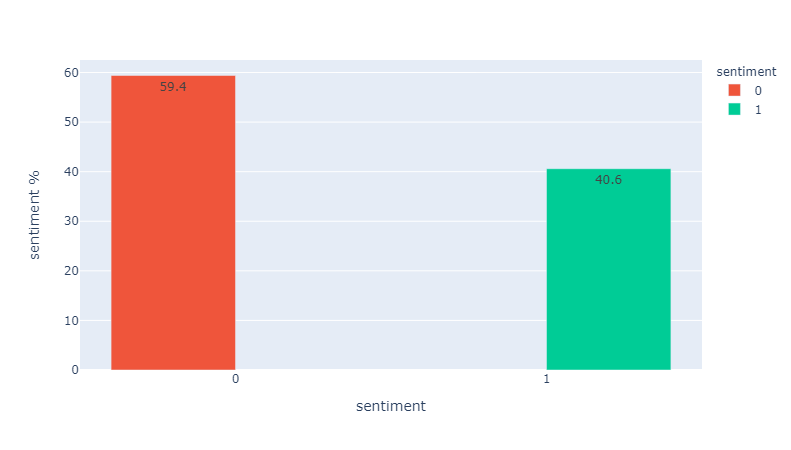
\includegraphics[width=1\textwidth]{images/output_68_0.png}
\caption{Total positive vs negative}
\label{fig:fig_tot}
\end{figure}
\FloatBarrier

The y-axis describes the percentage of all articles by sentiment, which are located on the x-axis.
\textbf{Comments}:
It is visible that almost 60\% of the articles were classified with negative sentiment.

\subsubsection{Plot of all newspaper positive vs negative}
\label{chap:allposneg}
The plot in Figure~\ref{fig:fig_all} describes the positive and negative percentage of all newspapers that have more than 20 articles, I used this filter to get more accurate statistics. Newspapers with a few articles in fact would have biased the analysis.
\begin{figure}[H]
\centering
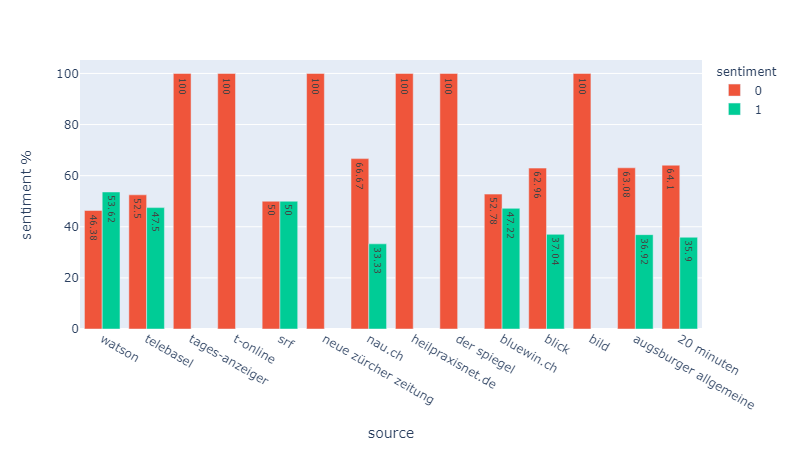
\includegraphics[width=1\textwidth]{images/output_79_0.png}
\caption{Newspaper sentiment}
\label{fig:fig_all}
\end{figure}
\FloatBarrier
The y-axis indicates the percentage of positive or negative sentiment, categorized by the sources located on the x-axis.
\textbf{Comments}:
Interesting to see that some newspapers have a negativity of 100\%.

\subsubsection{Plot top 10 newspaper positive}
The plot in Figure~\ref{fig:fig_10pos} shows the best positive papers. The dataframe from section \ref{chap:allposneg} was used here, so newspapers below a certain number of articles are not considered.
\begin{figure}[H]
\centering
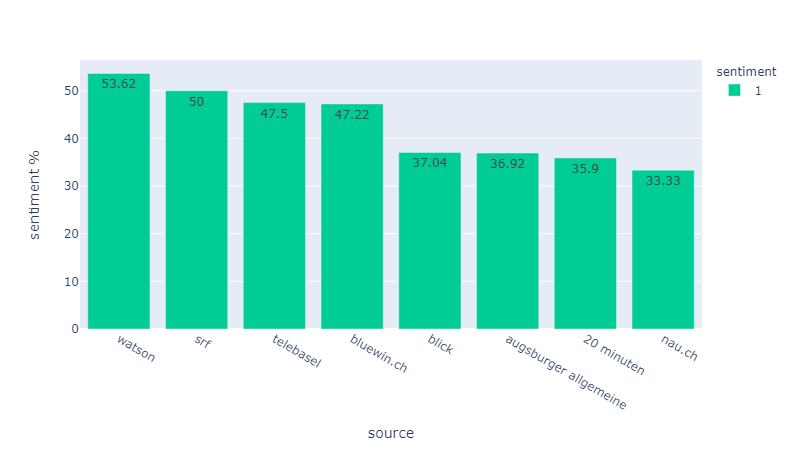
\includegraphics[width=1\textwidth]{images/output_85_0.png}
\caption{Top 10 positive}
\label{fig:fig_10pos}
\end{figure}
\FloatBarrier
The y-axis shows the percentage of all positive items, divided by the sources located on the x-axis.
\textbf{Comments}:

\subsubsection{Plot top 10 newspaper negative}
The plot in Figure~\ref{fig:fig_10neg} shows the 10 most negative newspapers. Also here the dataframe from section \ref{chap:allposneg} was used.
\begin{figure}[H]
\centering
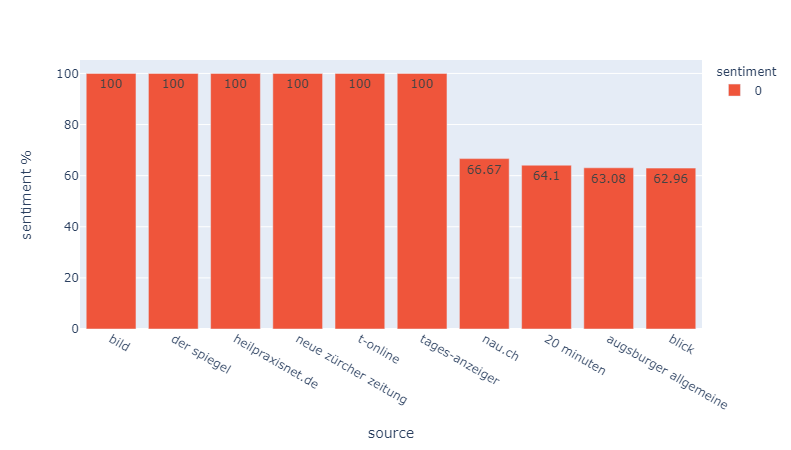
\includegraphics[width=1\textwidth]{images/output_86_0.png}
\caption{Top 10 negative}
\label{fig:fig_10neg}
\end{figure}
\FloatBarrier
The y-axis shows the percentage of all negative items, divided by the sources located on the x-axis.
\textbf{Comments}:


\subsubsection{Plot pro category positive vs negative}
The plot in Figure~\ref{fig:fig_catposneg} is used to see the percentage of positivity and negativity of each category without considering the newspapers. Thanks to the grouping function I was able to group each individual category and then normalized.

\begin{figure}[H]
\centering
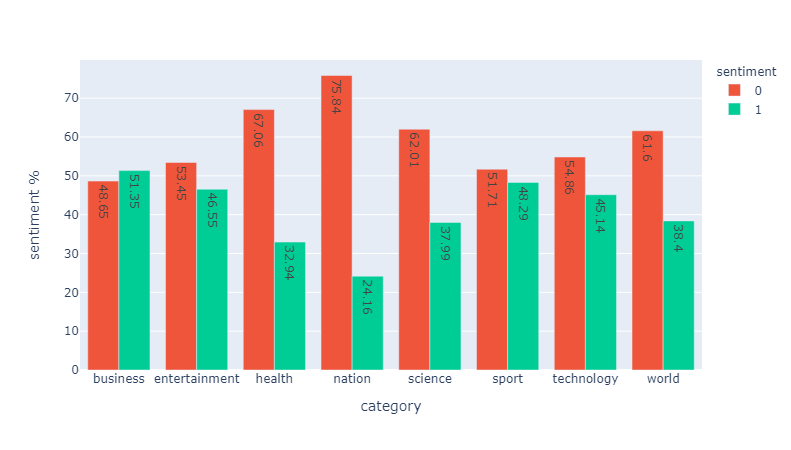
\includegraphics[width=1\textwidth]{images/output_91_0.png}
\caption{Category positive vs negative}
\label{fig:fig_catposneg}
\end{figure}
\FloatBarrier
The y-axis indicates the percentage of positive or negative sentiment, sorted by the categories located on the x-axis.
\textbf{Comments}: Si può notare che la categoria "nome categoria" sia quella messa peggio con ben "percentuale" di articoli negativi.

\subsubsection{Plot pro category of the top 3 newspaper}
The plot in Figure~\ref{fig:fig_top3} is used to see the percentage of positivity and negativity of the three largest newspapers by number of articles, all grouped by category.

\begin{figure}[H]
\centering
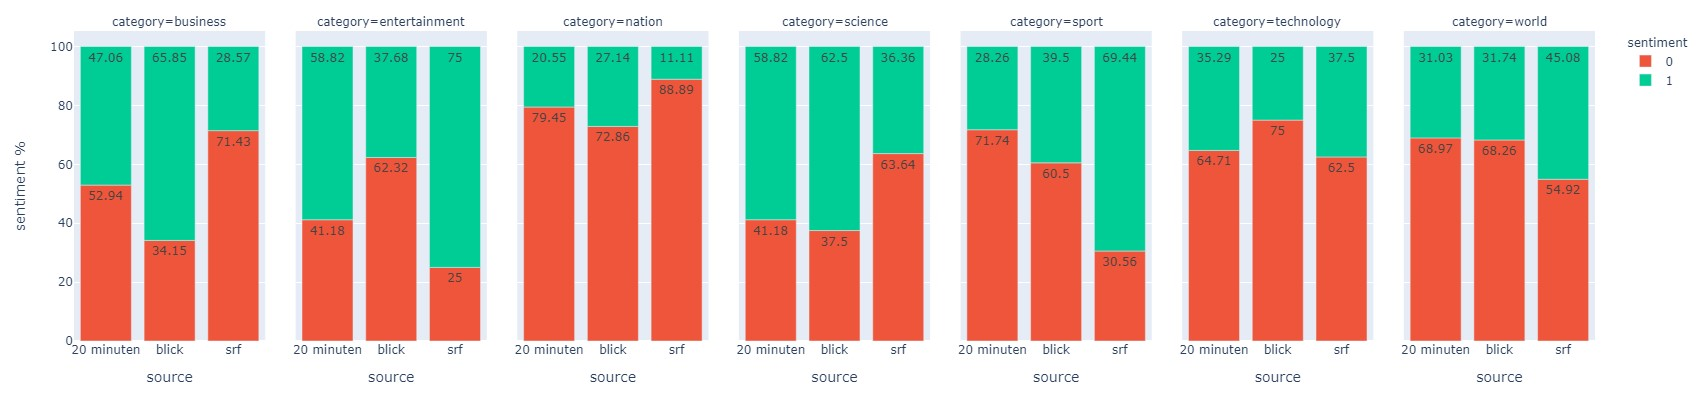
\includegraphics[width=1.0\textwidth]{images/cat2.jpg}
\caption{Top 3 newspaper}
\label{fig:fig_top3}
\end{figure}
\FloatBarrier

Then I wanted to create a plot that is an improvement of the previous one. In fact, I have assigned to the values of the negative sentiment a negative value.
The plot in Figure~\ref{fig:fig_improvement} is therefore clearer.

\begin{figure}[H]
\centering
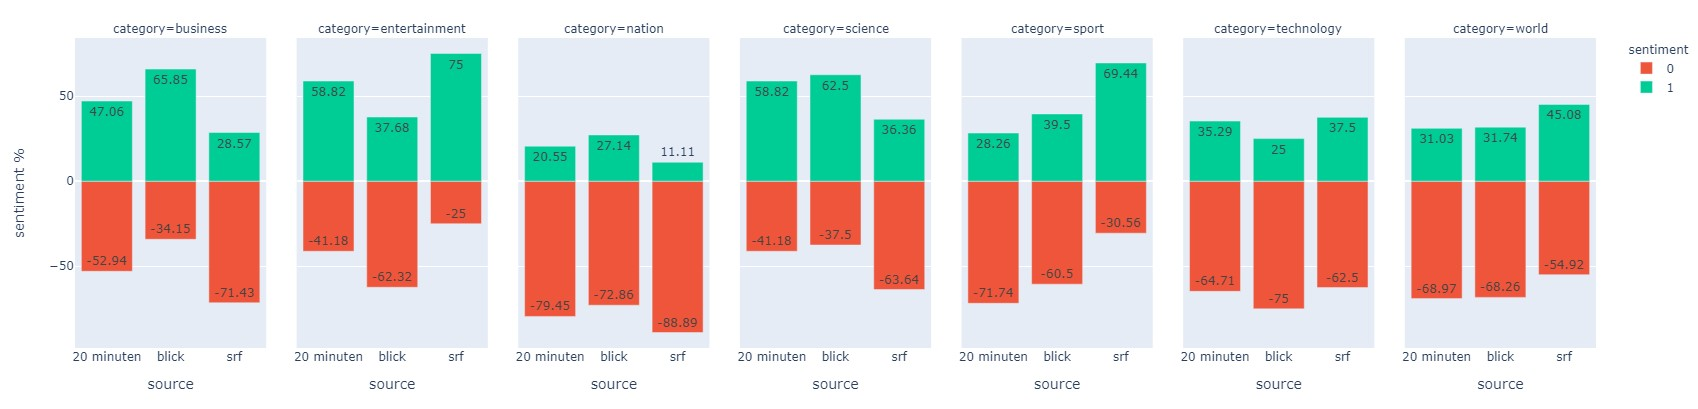
\includegraphics[width=1.0\textwidth]{images/cat.jpg}
\caption{Top 3 newspaper improvement}
\label{fig:fig_improvement}
\end{figure}
\FloatBarrier
\textbf{Comments}: Si può notare che la categoria "nome categoria" sia quella messa peggio con ben "percentuale" di articoli negativi.

\subsubsection{Plot spider category of a single newspaper} 
The plot in Figure~\ref{fig:fig_spider} gives an idea of the area that each newspaper covers based on the categories. I then created a function to be able to easily plot a list of given newspapers, without having to write everything by hand.

\begin{figure}[H]
\centering
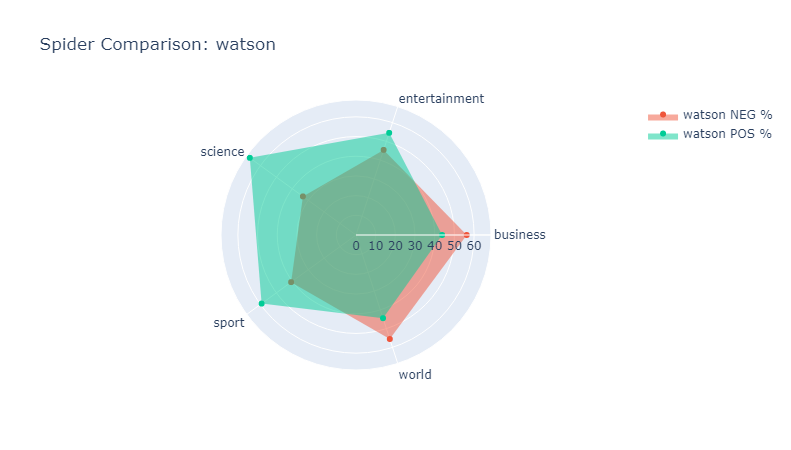
\includegraphics[width=1\textwidth]{images/output_110_9.png}
\caption{Newspaper spider}
\label{fig:fig_spider}
\end{figure}
\FloatBarrier
Each point on the plot equals the percentage of positivity (in green) or negativity (in red) of a given category. By connecting all the points I define the area of positivity and negativity of each newspaper.

\textbf{Comments}: Si può notare che la categoria "nome categoria" sia quella messa peggio con ben "percentuale" di articoli negativi.


\subsubsection{Plot in time newspaper} 
The plot in Figure~\ref{fig:fig_timenews} shows the trend of a newspaper over time.
The top 3 newspapers were chosen because they are the ones that influence the most in the Swiss territory.
The time span is from May 1, 2021 until today.

\begin{figure}[H]
\centering
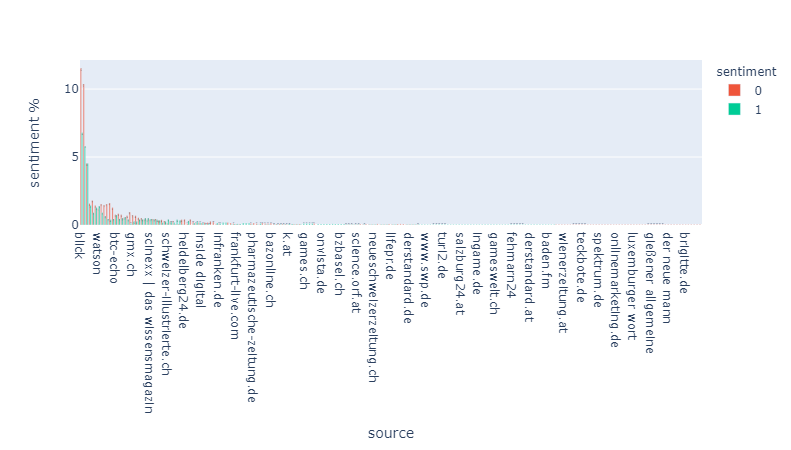
\includegraphics[width=1\textwidth]{images/output_71_0.png}
\caption{Newspaper in time}
\label{fig:fig_timenews}
\end{figure}
\FloatBarrier

The plot presents on the x-axis the time range, and on the y-axis the percentage of positivity or negativity that a paper had over a single day.
Each newspaper then is divided into two colors in order to distinguish the positive and negative sentiment. For the division of colors I took into consideration per newspaper two similar colors. The darker color of the two represents positive sentiment, the lighter color represents negative sentiment.

\subsubsection{Plot in time category}
The plot in Figure~\ref{fig:fig_cattime} is an interesting plot because it shows the trend over time as events occur.

\begin{figure}[H]
\centering
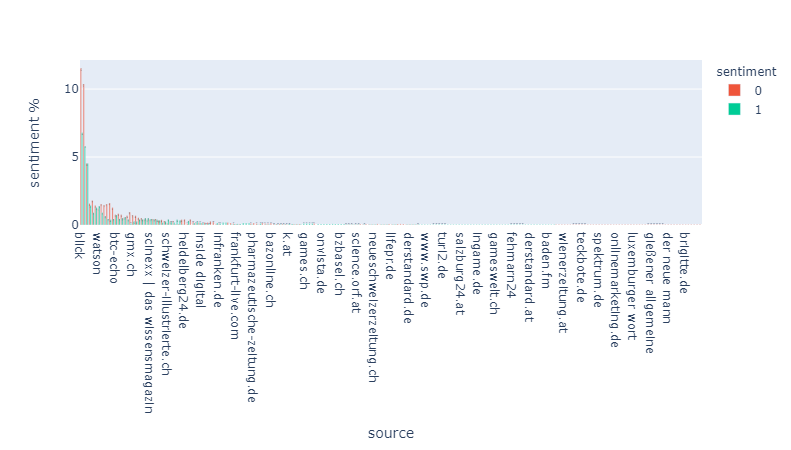
\includegraphics[width=1\textwidth]{images/output_71_0.png}
\caption{Category in time}
\label{fig:fig_cattime}
\end{figure}
\FloatBarrier

The plot presents on the x-axis the time range, and on the y-axis the percentage of positivity or negativity that a category had over a single day.
Each category is divided into two colors in order to distinguish positive and negative feeling. For the subdivision of colors I have taken into consideration per category two similar colors. The darker color of the two represents positive sentiment, the lighter color represents negative sentiment.

Recently, negative events have occurred between Palestine and Israel. As of May 17, the category world has had a boost in negative sentiment. It would have been nice to see the performance of the newspapers before and during the pandemic. 
Being the end of May, maybe I am lucky enough to see the change in direction of the pandemic, like last year in fact in summer it has less effect. Taking into consideration also the vaccination campaign, I speculate that it will be possible to see an improvement in the situation in almost all categories of newspaper. 


\section{Challenges}
In diesem Abschnitt befassen wir uns mit den Herausforderungen, die sich während der Arbeit am Projekt herausgestellt haben, und wir diese behandelt haben.

\subsubsection*{Finden des geeigneten \gls{dataset}s} 
Unser erstes Problem war es, einen passenden Datensatz für unsere Bedürfnisse zu finden. Um ein Modell zu trainieren, brauchten wir einen Datensatz, der für die Sentiment-Analyse relevant, aber auch gross genug war, um ihn in Trainings- und Test-Sets aufzuteilen, ohne die Modellqualität zu verlieren. Zu unseren Gunsten hat Kaggle reichlich viele Beispiele von guten Datensätzen.

\subsubsection*{\gls{virtual machine}}
Unser zweites Problem bezieht sich auf unsere virtuelle Maschine. Diese war anfangs hardware-technisch nicht zureichend für unser Projekt ausgestattet, da unser Projekt sehr rechenintensive Programme verwendet. Nach Anfrage auf eine leistungsstärkere Maschine wurde dieses Problem gelöst. In der Zwischenzeit, sind wir wieder zu Google \gls{colab} umgezogen, dort waren bereits viele Abhängigkeiten installiert.

\subsubsection*{Google \gls{colab}}
Ein Problem, das wir mit \gls{colab} hatten, war, dass wir jedes Mal, wenn wir das Notebook öffneten, das \gls{dataset} neu importieren mussten. Dies nam jeweils eine grosse Menge an Zeit in Anspruch, da unser \gls{dataset} sehr gross ist. Wir haben auch versucht, \gls{colab} auf der virtuellen Maschine laufen zu lassen, aber \gls{colab} stoppt automatisch nach einer bestimmten Zeit die Ausführung, was nicht ideal für unsere Arbeit war, da das Trainieren eines Modells bis zu mehreren Stunden andauern kann. Letzten Endes stellte sich Anaconda als die geeignete Lösung hervor.

\subsubsection*{\gls{anaconda} und \gls{jupyter}}
Beim Übergang von \gls{colab} auf die \gls{virtual machine}, haben wir bei \gls{colab} eine Datei mit allen benötigten Libraries exportiert. Daraus haben wir auf der virtuellen Maschine mit \gls{anaconda} versucht, eine neue Umgebung zu erstellen, die alle Libraries von \gls{colab} enthält. Jedoch schlug die Ausführung mit \gls{anaconda} fehl, aufgrund eines Versionskonfliktes zwischen den Libraries. Womöglich hatte dieser Fehler einen Zusammenhang mit fehlenden Zugriffsrechten in der Systemadministration. Dementsprechend verwarfen wir die Idee eine neue Umgebung zu erstellen und arbeiteten auf der Standardumgebung von \gls{anaconda}, auf der alles ohne Probleme verlief.

\subsubsection*{Grosse Verarbeitungszeiten}
Sowohl auf \gls{colab} als auch lokal auf der virtuellen Maschine mit \gls{anaconda} ist die Verarbeitungsdauer der Datensätze mit dem Sentence Encoder mehrere Stunden lang. Um lange Wartezeiten zu umgehen, haben wir des Öfteren mit verkürzten Versionen unseres \gls{dataset}s gearbeitet. Für das finale Produkt, ist jedoch eine grosse Anzahl an Daten erforderlich, weshalb wir gegen Ende des Projektes unser Sentiment-Analysis-Model nochmals mit der ganzen Menge an Daten gefüttert haben.




\section{Conclusion}
Im jetzigen Zustand haben wir ein funktionierendes Sentiment-Analysis-Model, welches einen Text lesen und ein Sentiment dazu abgeben kann, welches sich in einem Rahmen von 5 verschiedenen Kategorien befindet. Die Genauigkeit, oder die Wahrscheinlichkeit die richtige Kategorie zu treffen, liegt dabei bei rund 60\%. Das Model ist dazu trainiert ganze Sätze zu verarbeiten. Bei einzelnen Worten könnte es deshalb etwas willkürliche Resultate ausgeben. Momentan ist das Model noch an ein Jupyter-Notebook gebunden, im nächsten Schritt jedoch, würde man dieses Model exportieren und in eine serverseitige Applikation einbinden, welche sich beispielsweise über eine API aufrufen lässt.

\section{Attachments}
In addition to the documentation, the following documents are available:
\begin{itemize}
    \item \textbf{"SentimentOnSwissNewspaper.html"}, the source code of the project in html format
    \item \textbf{"SentimentOnSwissNewspaper.pdf"}, the source code of the project in pdf format
    \item \textbf{"SentimentOnSwissNewspaper.pdf"}, the schedule of the project in pdf format
    \item \textbf{"SentimentOnSwissNewspaper.xlsx"}, the schedule of the project in excel format
    \item \textbf{"Arbeitsaufteilungein.docx"}, die Word-Datei für die Unterteilung der Kapitel
\end{itemize}


\newpage\leavevmode\thispagestyle{plain}\newpage
%---------------------------------------------------------------------------
% Appendix
%---------------------------------------------------------------------------
\clearpage
\phantomsection 
\appendix
\section{Appendix : Models created}
In addition to the documentation, I have described in this section all the models I have created over time.
From each model I learned something and realized what I could improve.
The models are listed from first to second to last to show the learning journey.

\subsection{First model: IMDb dataset}
The first model I created was with \gls{BERT}, without any framework I simply followed the official \gls{Tensorflow} tutorial.
I trained this model the IMDb dataset.
This model was purely for educational purposes, once trained the model the only work that actually there was to do was a little fine tuning.
I used this model only as an approach to get into the world of \gls{BERT}, in fact I followed the tutorial of \gls{Tensorflow} itself to get to this result.
For a thesis work I wanted to do something of my own, and not using code and tutorial that it can already find on the net, so I tried something different.
After several searches I came across \gls{Ktrain}.

\subsubsection{Lesson learned}
I learned how to configure a model with the optimizer, loss and metric.

\textbf{What is optimizer?}\\
Optimizers are used for improving speed and performance for training a specific model \cite{noauthor_tensorflow_nodate_optimizer}. 
For my model I chose Adam optimizer. Adam optimization is a stochastic gradient descent method that is based on adaptive estimation of first order and second-order moments \cite{noauthor_tfkerasoptimizersadam_nodate}.

\textbf{What is loss?}\\
 We use a loss function to determine how far the predicted values deviate from the actual values in the training data. We change the model weights to make the loss minimum, and that is what training is all about \cite{patnaik_loss_2018}.
 
\textbf{What is a metric?}\\Calculates how often predictions matches integer labels \cite{noauthor_tfkerasmetricssparsecategoricalaccuracy_nodate}.

\subsection{Second model: Ktrain - Hotel dataset}
To be able to do something of my own I thought to work also on the dataset, so with \gls{Ktrain} I did not use the IMDB dataset, but I opted for the Hotel Reviews dataset.

\subsubsection{Hotel Review Dataset}
\paragraph*{Dataframe structure}
The CSV file contains 17 columns, this means that one customer rating contains 17 attributes. In Table~\ref{tab:Dataframe structure} all attributes are explained in detail:

\begin{longtable}[ c ]{| m{5cm} | m{8cm}|}
\hline
\multicolumn{2}{|c|}{\textbf{Dataframe structure}}                                                                                                         \\ \hline
\endfirsthead
%
\multicolumn{2}{c}%
{{\bfseries  Table \thetable\ continued from previous page}} \\
\hline
\multicolumn{2}{|c|}{\textbf{Dataframe structure}}                                                                                                         \\ \hline
\endhead
%
\textbf{Hotel\_Address  }                     & Hotel address.                                                                                  \\ \hline
\textbf{Review\_Date}                         & Date on which the customer left his comment.                                          \\ \hline
\textbf{Average\_Score}                       & Average rating. Calculation by all comments of the last year.              \\ \hline
\textbf{Hotel\_Name}                          & Hotel name.                                                                                     \\ \hline
\textbf{Reviewer\_Nationality}                & Client nationality.                                                                             \\ \hline
\textbf{Negative\_Review}                     & Negative review of the customer. If there is no negative review, it says: "No Negative". \\ \hline
\textbf{ReviewTotalNegativeWord Counts}        & Number of words in the negative review.                                                        \\ \hline
\textbf{Positive\_Review}                     & Positive review of the customer. If there is no positive review, it says: "No Positive". \\ \hline
\textbf{ReviewTotalPositiveWord Counts}        & Number of words in the positive review.                                                        \\ \hline
\textbf{Reviewer\_Score}                      & Score Rating.                                                                                \\ \hline
\textbf{TotalNumberofReviews ReviewerHasGiven} & Total number of reviews left by the customer.                                  \\ \hline
\textbf{TotalNumberof\_Reviews}               & Number of reviews of the hotel.                                                                   \\ \hline
\textbf{Tags}                                 & Tags left by the customer for the review.                                                 \\ \hline
\textbf{dayssincereview}                      & Number of days between the evaluation date and creation of the \gls{dataset}.                              \\ \hline
\textbf{AdditionalNumberof \_Scoring} & The number of reviews of the customer, which consist only of a score rating and do not include a comment. \\ \hline
\textbf{lat}                                  & Latitude of the location of the hotel.                                                                 \\ \hline
\textbf{lng}                                  & Longitude of the location of the hotel.                                                                  \\ \hline
\caption{Dataframe structure}
\label{tab:Dataframe structure}\\
\end{longtable}

\subsubsection{Process the data}
To do this first I worked on the dataset so:
\begin{itemize}
    \item cleaned up the columns I did not need,
    \item divided the dataset in positive and negative thanks to the score table, so for a value below 7 is negative and above 7 is positive,
    \item resample so that there are the same number of reviews for positive and negative.
\end{itemize}

\gls{Ktrain} provides me with a lot of useful features for my purpose.
The first \gls{Ktrain} function I used is text.texts\_from\_df.
As it is written in the documentation \cite{noauthor_amaiyaktrain_nodate}, this function allows me to:

“Loads text data from \gls{Pandas} dataframe file. Class labels are assumed to be one of the following formats:
\begin{itemize}
    \item one-hot-encoded or multi-hot-encoded arrays representing classes
    \item labels are in a single column of string or integer values representing class labels
    \item labels are a single column of numerical values for text regression.”
\end{itemize}
The advantage is that I do not have to do every single preprocessing step manually, and all the steps are followed by the library itself.

Mine is case number two, in fact my dataframe in Figure~\ref{fig:fig_24}, is composed as follows:
\begin{figure}[ht!]
\centering
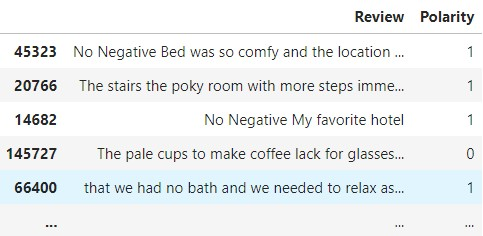
\includegraphics[width=0.65\textwidth]{images/dataframe.jpg}
\caption{My resample dataframe}
\label{fig:fig_24}
\end{figure}
\FloatBarrier

In Figure~\ref{fig:fig_22} shown the function from the documentation and the code function I used:
\begin{figure}[ht!]
\centering
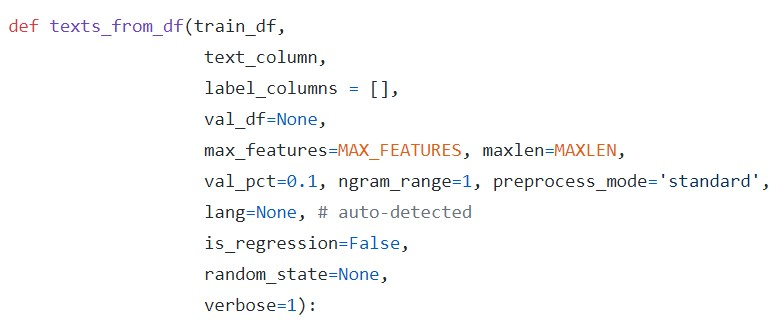
\includegraphics[width=0.75\textwidth]{images/textdf.jpg}
\caption{\gls{Ktrain} text function from documentation}
\label{fig:fig_22}
\end{figure}
\FloatBarrier
The function will take as feature the column "Review" and as target "Polarity", it will also automatically download an already pretrained DistilBERT model with its vocabulary.
The data for the DistilBERT model has to be preprocessed in a certain way, so I have to indicate this at the preprocess\_mode line.
    \begin{tcolorbox}[breakable, size=fbox, boxrule=1pt, pad at break*=1mm,colback=cellbackground, colframe=cellborder]

\begin{Verbatim}[commandchars=\\\{\},fontsize=\footnotesize]
\PY{n}{train}\PY{p}{,} \PY{n}{val}\PY{p}{,} \PY{n}{preproc} \PY{o}{=} \PY{n}{text}\PY{o}{.}\PY{n}{texts\PYZus{}from\PYZus{}df}\PY{p}{(}
\PY{n}{train\PYZus{}df}\PY{o}{=}\PY{n}{train}\PY{p}{,}
\PY{n}{text\PYZus{}column}\PY{o}{=}\PY{l+s+s1}{\PYZsq{}}\PY{l+s+s1}{Review}\PY{l+s+s1}{\PYZsq{}}\PY{p}{,}
\PY{n}{label\PYZus{}columns}\PY{o}{=}\PY{l+s+s1}{\PYZsq{}}\PY{l+s+s1}{Polarity}\PY{l+s+s1}{\PYZsq{}}\PY{p}{,}
\PY{n}{val\PYZus{}df}\PY{o}{=}\PY{n}{test}\PY{p}{,}
\PY{n}{maxlen}\PY{o}{=}\PY{l+m+mi}{400}\PY{p}{,}
\PY{n}{preprocess\PYZus{}mode}\PY{o}{=}\PY{l+s+s1}{\PYZsq{}}\PY{l+s+s1}{distilbert}\PY{l+s+s1}{\PYZsq{}}
\PY{p}{)}
\end{Verbatim}
\end{tcolorbox}

\begin{Verbatim}[commandchars=\\\{\},fontsize=\footnotesize]
['not\_Polarity', 'Polarity']
        not\_Polarity  Polarity
128508           1.0       0.0
78547            0.0       1.0
131921           1.0       0.0
16602            0.0       1.0
134008           1.0       0.0
['not\_Polarity', 'Polarity']
        not\_Polarity  Polarity
45323            0.0       1.0
20766            0.0       1.0
14682            0.0       1.0
145727           1.0       0.0
66400            0.0       1.0
preprocessing train{\ldots}
language: en
train sequence lengths:
        mean : 39
        95percentile : 120
        99percentile : 227
    \end{Verbatim}

    
    \begin{Verbatim}[commandchars=\\\{\},fontsize=\footnotesize]
<IPython.core.display.HTML object>
    \end{Verbatim}

    
    \begin{Verbatim}[commandchars=\\\{\},fontsize=\footnotesize]
Is Multi-Label? False
preprocessing test{\ldots}
language: en
test sequence lengths:
        mean : 40
        95percentile : 123
        99percentile : 225
    \end{Verbatim}
So with this function I load the dataframe that I processed (hotel), I use the Review column for the text to process, while I use the Polarity column to get my target.


\subsubsection{Build a Model and Wrap in Learner}
\paragraph{Classifier}
In this section is described the construction of the model, to do this first I had to see what classifier \gls{Ktrain} allows me to have:
    \begin{tcolorbox}[breakable, size=fbox, boxrule=1pt, pad at break*=1mm,colback=cellbackground, colframe=cellborder]
\begin{Verbatim}[commandchars=\\\{\},fontsize=\footnotesize]
\PY{n}{text}\PY{o}{.}\PY{n}{print\PYZus{}text\PYZus{}classifiers}\PY{p}{(}\PY{p}{)}
\end{Verbatim}
\end{tcolorbox}

    \begin{Verbatim}[commandchars=\\\{\},fontsize=\footnotesize]
fasttext: a fastText-like model [http://arxiv.org/pdf/1607.01759.pdf]
logreg: logistic regression using a trainable Embedding layer
nbsvm: NBSVM model [http://www.aclweb.org/anthology/P12-2018]
bigru: Bidirectional GRU with pretrained fasttext word vectors
[https://fasttext.cc/docs/en/crawl-vectors.html]
standard\_gru: simple 2-layer GRU with randomly initialized embeddings
bert: Bidirectional Encoder Representations from Transformers (\gls{BERT}) from
keras\_bert [https://arxiv.org/abs/1810.04805]
distilbert: distilled, smaller, and faster \gls{BERT} from Hugging Face transformers
[https://arxiv.org/abs/1910.01108]
    \end{Verbatim}

The classifier I need is distilbert. DistilBERT \cite{sanh_distilbert_2020} is a distilled version of \gls{BERT}, in fact it reduces the size of \gls{BERT} by 40\%, while retaining 97\% of its language understanding capabilities and being 60\% faster.

So it is smaller and faster implemented by \gls{Hugging Face} transformer \cite{noauthor_distilbert_nodate}.
To be able to use the text.text\_classifier function I helped myself with its documentation using some help directly in Jupyter file:
 \begin{tcolorbox}[breakable, size=fbox, boxrule=1pt, pad at break*=1mm,colback=cellbackground, colframe=cellborder]
\begin{Verbatim}[commandchars=\\\{\},fontsize=\footnotesize]
\PY{n}{help}\PY{p}{(}\PY{n}{text}\PY{o}{.}\PY{n}{text\PYZus{}classifier}\PY{p}{)}
\end{Verbatim}
\end{tcolorbox}

    \begin{Verbatim}[commandchars=\\\{\},fontsize=\footnotesize]
Help on function text\_classifier in module ktrain.text.models:

text\_classifier(name, train\_data, preproc=None, multilabel=None,
metrics=['accuracy'], verbose=1)
    Build and return a text classification model.

    Args:
        name (string): one of:
                    - 'fasttext' for FastText model
                    - 'nbsvm' for NBSVM model
                    - 'logreg' for logistic regression using embedding layers
                    - 'bigru' for Bidirectional GRU with pretrained word vectors
                    - 'bert' for \gls{BERT} Text Classification
                    - 'distilbert' for Hugging Face DistilBert model

        train\_data (tuple): a tuple of numpy.ndarrays: (x\_train, y\_train) or
ktrain.Dataset instance
                        returned from one of the texts\_from\_* functions
        preproc: a ktrain.text.TextPreprocessor instance.
                 As of v0.8.0, this is required.
        multilabel (bool):  If True, multilabel model will be returned.
                            If false, binary/multiclass model will be returned.
                            If None, multilabel will be inferred from data.
        metrics(list): metrics to use
        verbose (boolean): verbosity of output
    Return:
        model (Model): A \gls{Keras} Model instance

    \end{Verbatim}

Now that I know how it works, I can build my model so, I chose the classifier (distilbert), train data and preproc are the data I created in the previous function, putting everything together I have as shown in code:
    \begin{tcolorbox}[breakable, size=fbox, boxrule=1pt, pad at break*=1mm,colback=cellbackground, colframe=cellborder]
\begin{Verbatim}[commandchars=\\\{\},fontsize=\footnotesize]
\PY{n}{model} \PY{o}{=} \PY{n}{text}\PY{o}{.}\PY{n}{text\PYZus{}classifier}\PY{p}{(}\PY{l+s+s1}{\PYZsq{}}\PY{l+s+s1}{distilbert}\PY{l+s+s1}{\PYZsq{}}\PY{p}{,} \PY{n}{train\PYZus{}data}\PY{o}{=}\PY{n}{train}\PY{p}{,} \PY{n}{preproc}\PY{o}{=}\PY{n}{preproc}\PY{p}{)}
\end{Verbatim}
\end{tcolorbox}

\paragraph{get\_learner}
Now that I have a model, I can create a learner:
    \begin{tcolorbox}[breakable, size=fbox, boxrule=1pt, pad at break*=1mm,colback=cellbackground, colframe=cellborder]
\begin{Verbatim}[commandchars=\\\{\},fontsize=\footnotesize]
\PY{n}{learner} \PY{o}{=} \PY{n}{ktrain}\PY{o}{.}\PY{n}{get\PYZus{}learner}\PY{p}{(}\PY{n}{model}\PY{p}{,}
                             \PY{n}{train\PYZus{}data}\PY{o}{=}\PY{n}{train}\PY{p}{,} 
                             \PY{n}{val\PYZus{}data}\PY{o}{=}\PY{n}{val}\PY{p}{,} 
                             \PY{n}{batch\PYZus{}size}\PY{o}{=}\PY{l+m+mi}{6}\PY{p}{)}
\end{Verbatim}
\end{tcolorbox}

\paragraph{learner.lr\_find and plot()}
Now I simulate a workout on different learning rates and its \gls{plot} in figure~\ref{fig:fig_29}, using the functions:
    \begin{tcolorbox}[breakable, size=fbox, boxrule=1pt, pad at break*=1mm,colback=cellbackground, colframe=cellborder]
\begin{Verbatim}[commandchars=\\\{\},fontsize=\footnotesize]
\PY{n}{learner}\PY{o}{.}\PY{n}{lr\PYZus{}find}\PY{p}{(}\PY{p}{)}
\end{Verbatim}
\end{tcolorbox}

\begin{tcolorbox}[breakable, size=fbox, boxrule=1pt, pad at break*=1mm,colback=cellbackground, colframe=cellborder]
\begin{Verbatim}[commandchars=\\\{\},fontsize=\footnotesize]
\PY{n}{learner}\PY{o}{.}\PY{n}{lr\PYZus{}plot}\PY{p}{(}\PY{p}{)}
\end{Verbatim}
\end{tcolorbox}

\begin{figure}[ht!]
\centering
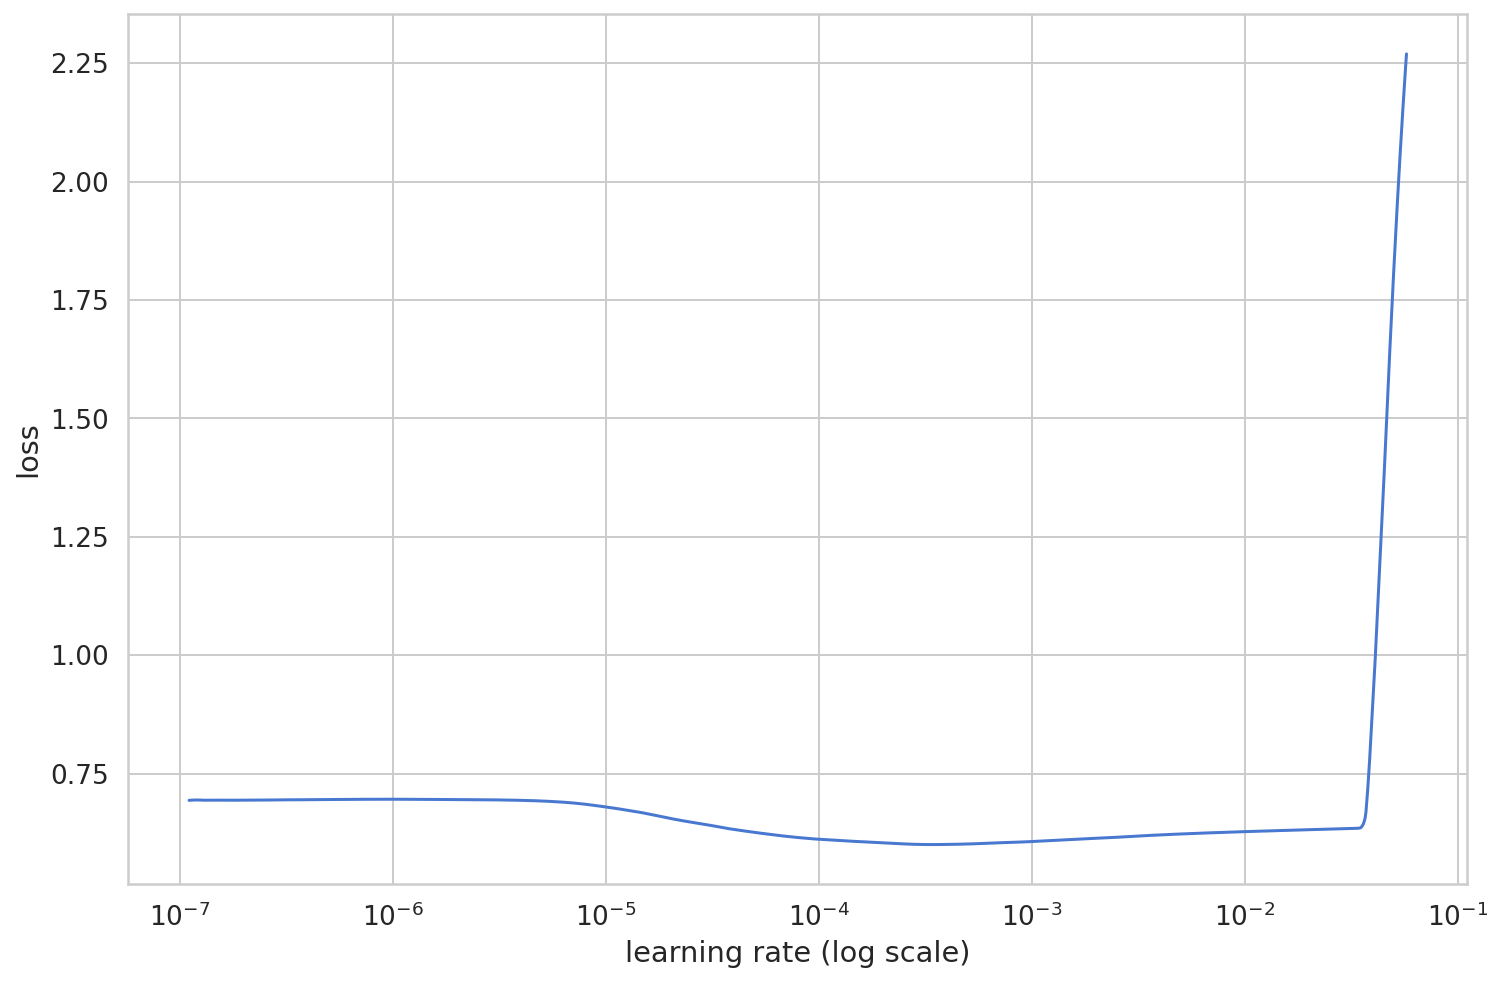
\includegraphics[width=1\textwidth]{images/output_97_0.png}
\caption{\gls{Ktrain} learner plot}
\label{fig:fig_29}
\end{figure}
\FloatBarrier

\paragraph{fit\_onecycle}
The fit\_onecycle method is better in speed and \gls{accuracy} as just the fit method.
The fit\_onecycle is an implementation of Leslie Smith’s 1cycle policy \cite{smith_disciplined_2018}.
By using the function:
    \begin{tcolorbox}[breakable, size=fbox, boxrule=1pt, pad at break*=1mm,colback=cellbackground, colframe=cellborder]
\begin{Verbatim}[commandchars=\\\{\},fontsize=\footnotesize]
\PY{n}{learner}\PY{o}{.}\PY{n}{fit\PYZus{}onecycle}\PY{p}{(}\PY{n}{lr} \PY{o}{=} \PY{l+m+mf}{3e\PYZhy{}5}\PY{p}{,} \PY{n}{epochs}\PY{o}{=}\PY{l+m+mi}{4}\PY{p}{)}
\end{Verbatim}
\end{tcolorbox}

 \begin{Verbatim}[commandchars=\\\{\},fontsize=\footnotesize]
begin training using onecycle policy with max lr of 3e-05{\ldots}
Epoch 1/4
23270/23270 [==============================] - 2593s 110ms/step - loss: 0.3926 -
accuracy: 0.8214 - val\_loss: 0.3282 - val\_accuracy: 0.8553
Epoch 2/4
23270/23270 [==============================] - 2587s 110ms/step - loss: 0.3142 -
accuracy: 0.8632 - val\_loss: 0.3245 - val\_accuracy: 0.8584
Epoch 3/4
23270/23270 [==============================] - 2587s 110ms/step - loss: 0.2734 -
accuracy: 0.8844 - val\_loss: 0.3210 - val\_accuracy: 0.8600
Epoch 4/4
23270/23270 [==============================] - 2588s 110ms/step - loss: 0.1708 -
accuracy: 0.9318 - val\_loss: 0.4025 - val\_accuracy: 0.8537
    \end{Verbatim}
At the 4th epoch I have about 85\% \gls{accuracy}.

\paragraph{validate}
Using the:
    \begin{tcolorbox}[breakable, size=fbox, boxrule=1pt, pad at break*=1mm,colback=cellbackground, colframe=cellborder]
\begin{Verbatim}[commandchars=\\\{\},fontsize=\footnotesize]
\PY{n}{learner}\PY{o}{.}\PY{n}{validate}\PY{p}{(}\PY{p}{)}
\end{Verbatim}
\end{tcolorbox}method I can create a \gls{Confusion matrix} on the newly trained data in order to get a more detailed picture:
    \begin{Verbatim}[commandchars=\\\{\},fontsize=\footnotesize]
              precision    recall  f1-score   support

           0       0.85      0.86      0.85     17380
           1       0.86      0.85      0.85     17525

    accuracy                           0.85     34905
   macro avg       0.85      0.85      0.85     34905
weighted avg       0.85      0.85      0.85     34905

    \end{Verbatim}
            \begin{tcolorbox}[breakable, size=fbox, boxrule=.5pt, pad at break*=1mm, opacityfill=0]
\begin{Verbatim}[commandchars=\\\{\},fontsize=\footnotesize]
array([[14883,  2497],
       [ 2610, 14915]])
\end{Verbatim}
\end{tcolorbox}
        

\paragraph{autofit}
Not satisfied with this result I tried whit autofit \cite{noauthor_amaiyaktrainautofit_nodate}.
Next, I called the function as below:
    \begin{tcolorbox}[breakable, size=fbox, boxrule=1pt, pad at break*=1mm,colback=cellbackground, colframe=cellborder]
\begin{Verbatim}[commandchars=\\\{\},fontsize=\footnotesize]
\PY{n}{learner}\PY{o}{.}\PY{n}{autofit}\PY{p}{(}\PY{l+m+mf}{3e\PYZhy{}5}\PY{p}{,} \PY{n}{reduce\PYZus{}on\PYZus{}plateau}\PY{o}{=}\PY{l+m+mi}{3}\PY{p}{,} \PY{n}{checkpoint\PYZus{}folder}\PY{o}{=}\PY{l+s+s1}{\PYZsq{}}\PY{l+s+s1}{./checkpoint/}\PY{l+s+s1}{\PYZsq{}}\PY{p}{)}
\end{Verbatim}
\end{tcolorbox}

 \begin{Verbatim}[commandchars=\\\{\},fontsize=\footnotesize]
early\_stopping automatically enabled at patience=5

begin training using triangular learning rate policy with max lr of 3e-05{\ldots}
Epoch 1/1024
23270/23270 [==============================] - 2593s 110ms/step - loss: 0.1924 -
accuracy: 0.9222 - val\_loss: 0.4034 - val\_accuracy: 0.8520
\dots
Epoch 6/1024
23270/23270 [==============================] - 2588s 110ms/step - loss: 0.0412 -
accuracy: 0.9842 - val\_loss: 0.7817 - val\_accuracy: 0.8460
Restoring model weights from the end of the best epoch.
Epoch 00006: early stopping
Weights from best epoch have been loaded into model.
    \end{Verbatim}

\subsubsection{Discuss the limitations} 
As can be seen from the autofit code, also in this case I do not exceed 85\% \gls{accuracy} on validation data, having also here a problem of overfitting.

I then wanted to see what the data was where I had the most loss, this is possible due to:learner.view\_top\_losses(n=1),\\
with the result: id:11764 | loss:8.19 | true:1 | pred:0).\\
\\
At this point I saved the model and weights so that I would have a starting point for next time.\\
I made a list of improvements I want to make in the next test.\\
In text\_from\_df function:
\begin{itemize}
    \item label\_columns = must be a list, so I have to modify this argument,
    \item label\_columns = I can try wiht two different target columns positive and negative (so edit the dataframe),
    \item val\_df = none, so the 10\% of documents in training dataframe will be used for testing/validation,
    \item maxlen = from 400 to 500,
    \item random\_state = none, to have train/test split random.
\end{itemize}

I want also to use the Interactive Training \cite{jupyter_1204}.

\subsubsection{Lesson learned}
The most important of these improvements is missing, which is the work on the dataset.
In fact, the 85\% \gls{accuracy} is due to the fact of how I made the split between positive and negative reviews.


\subsection{Third model: Ktrain - Hotel dataset optimized}
The idea for this phase is to reduce the review window, focusing only on the actual negative reviews and the very positive reviews.
The continuation for this phase is as follows:
\begin{itemize}
    \item resume the original dataset,
    \item take only the best and worst reviews, based on the "Review\_Score" column,
    \item make a resample, so that you have the two categories in equal measure,
    \item and the other improvements described in the previous chapter.
\end{itemize}

\subsubsection{Improvements}
After making the improvements described above, I was able to create a model with an \gls{accuracy} for the English language of 96\%.

\subsection{Fourth model: Automatic Ktrain - Filmstarts dataset}
\label{chap:model filmstars auto}
In Switzerland the greater part of the newspaper articles are in German language, and for this reason the models that I have trained up to this moment are not suitable to the task that they must execute, therefore I have created a new model for the German language on the base of the previous models.
Fortunately, the basis I have for creating the model is correct, what I had to do is look for a suitable dataset.
For this assignment I chose a dataset on German movies, although it was difficult to find.
For training I did exactly the same as for the previous models, so I have:
\begin{itemize}
    \item clean the dataset,
    \item I have taken in consideration for the model only the more opportune data,
    \item trained model thanks to \gls{Ktrain}.
\end{itemize}

\subsubsection{Major changes}
For this model I used as in the previous \gls{Ktrain}, with these modifications:
\begin{itemize}
    \item \gls{BERT} instead of distilBERT for greater \gls{accuracy} with the German language,
    \item automatic model,
\end{itemize}
arriving at an \gls{accuracy} of 90\%.

\subsubsection{Discuss the limitations} 
Now that I have a trained model I tried testing with a file. The file consists of 30 news articles in German.

To do this test I manually labelled each item positive/negative creating a ground true and then compared it to what the model predicted.

What I saw was that the model correctly predicted most articles, with a few issues where the article was a fact or neutral, but this is normal since I only trained for positive and negative.
Unfortunately, despite the model arrives at a good percentage (90\%) I noticed that some articles where it is clearly negative were predicted positive. 

At this point I thought the problem was with the dataset and the model so here are the improvements I want to make in the next one:
\begin{itemize}
    \item take in consideration only 0 and 5 from the dataset,
    \item modify \gls{Ktrain}.
\end{itemize}
\section{Attachments}
In addition to the documentation, the following documents are available:
\begin{itemize}
    \item \textbf{"Task.pdf"}, the schedule of the project tasks in pdf format,
    \item \textbf{"BachelorTime.pdf"}, the schedule of the project in pdf format.
\end{itemize}

The code for the entire project, as well as the documentation and scripts, can be reached at the \gls{GitHub} repository of the bachelor thesis:\\
\url{https://github.com/bak89/Sentiment-Analysis-on-Swiss-Newspapers}

%\addcontentsline{toc}{section}{Index}
%\printindex
%---------------------------------------------------------------------------

% Declaration
%---------------------------------------------------------------------------
\clearpage
\phantomsection 
\addcontentsline{toc}{section}{Declaration of authorship}
\chapter*{Declaration of primary authorship}
\label{chap:declaration_authorship}

\vspace*{10mm} 

I / We hereby confirm that I / we have written this thesis independently and without using other sources and resources than those specified in the bibliography. All text passages which were not written by me are marked as quotations and provided with the exact indication of its origin. 

\vspace{15mm}

\begin{tabbing}
xxxxxxxxxxxxxxxxxxxxxxxxxxxxxx\=xxxxxxxxxxxxxxxxxxxxxxxxxxxxxx\=xxxxxxxxxxxxxxxxxxxxxxxxxxxxxx\kill
Place, Date:		\> [Biel/Burgdorf], \versiondate \\ \\ 
Last Name/s, First Name/s:	\> [Test Peter] 	\> [M\"uster R\"os\"a] \\ \\ \\ \\ 
Signature/s:	\> ......................................\> ...................................... \\
\end{tabbing}

%---------------------------------------------------------------------------

% Glossary
%---------------------------------------------------------------------------
\clearpage
\phantomsection 
\addcontentsline{toc}{section}{Index}
\printglossary[style=mcolindex, title=Index]%[type=\acronymtype]
%---------------------------------------------------------------------------

% Bibliography
%---------------------------------------------------------------------------
\clearpage
\phantomsection 
\addcontentsline{toc}{section}{References}
\printbibliography
%\bibliographystyle{IEEEtranS}
%\bibliographystyle{unsrt}
%\bibliography{database/references}
% Listings
%---------------------------------------------------------------------------
\clearpage
\phantomsection 
\addcontentsline{toc}{section}{List of figures}
\listoffigures
\clearpage
\phantomsection 
\addcontentsline{toc}{section}{List of tables}
\listoftables
%---------------------------------------------------------------------------

% Appendix
%---------------------------------------------------------------------------
\clearpage
\phantomsection 
\addcontentsline{toc}{section}{Attachments}

\includepdf[pages=-]{Attachments.pdf}
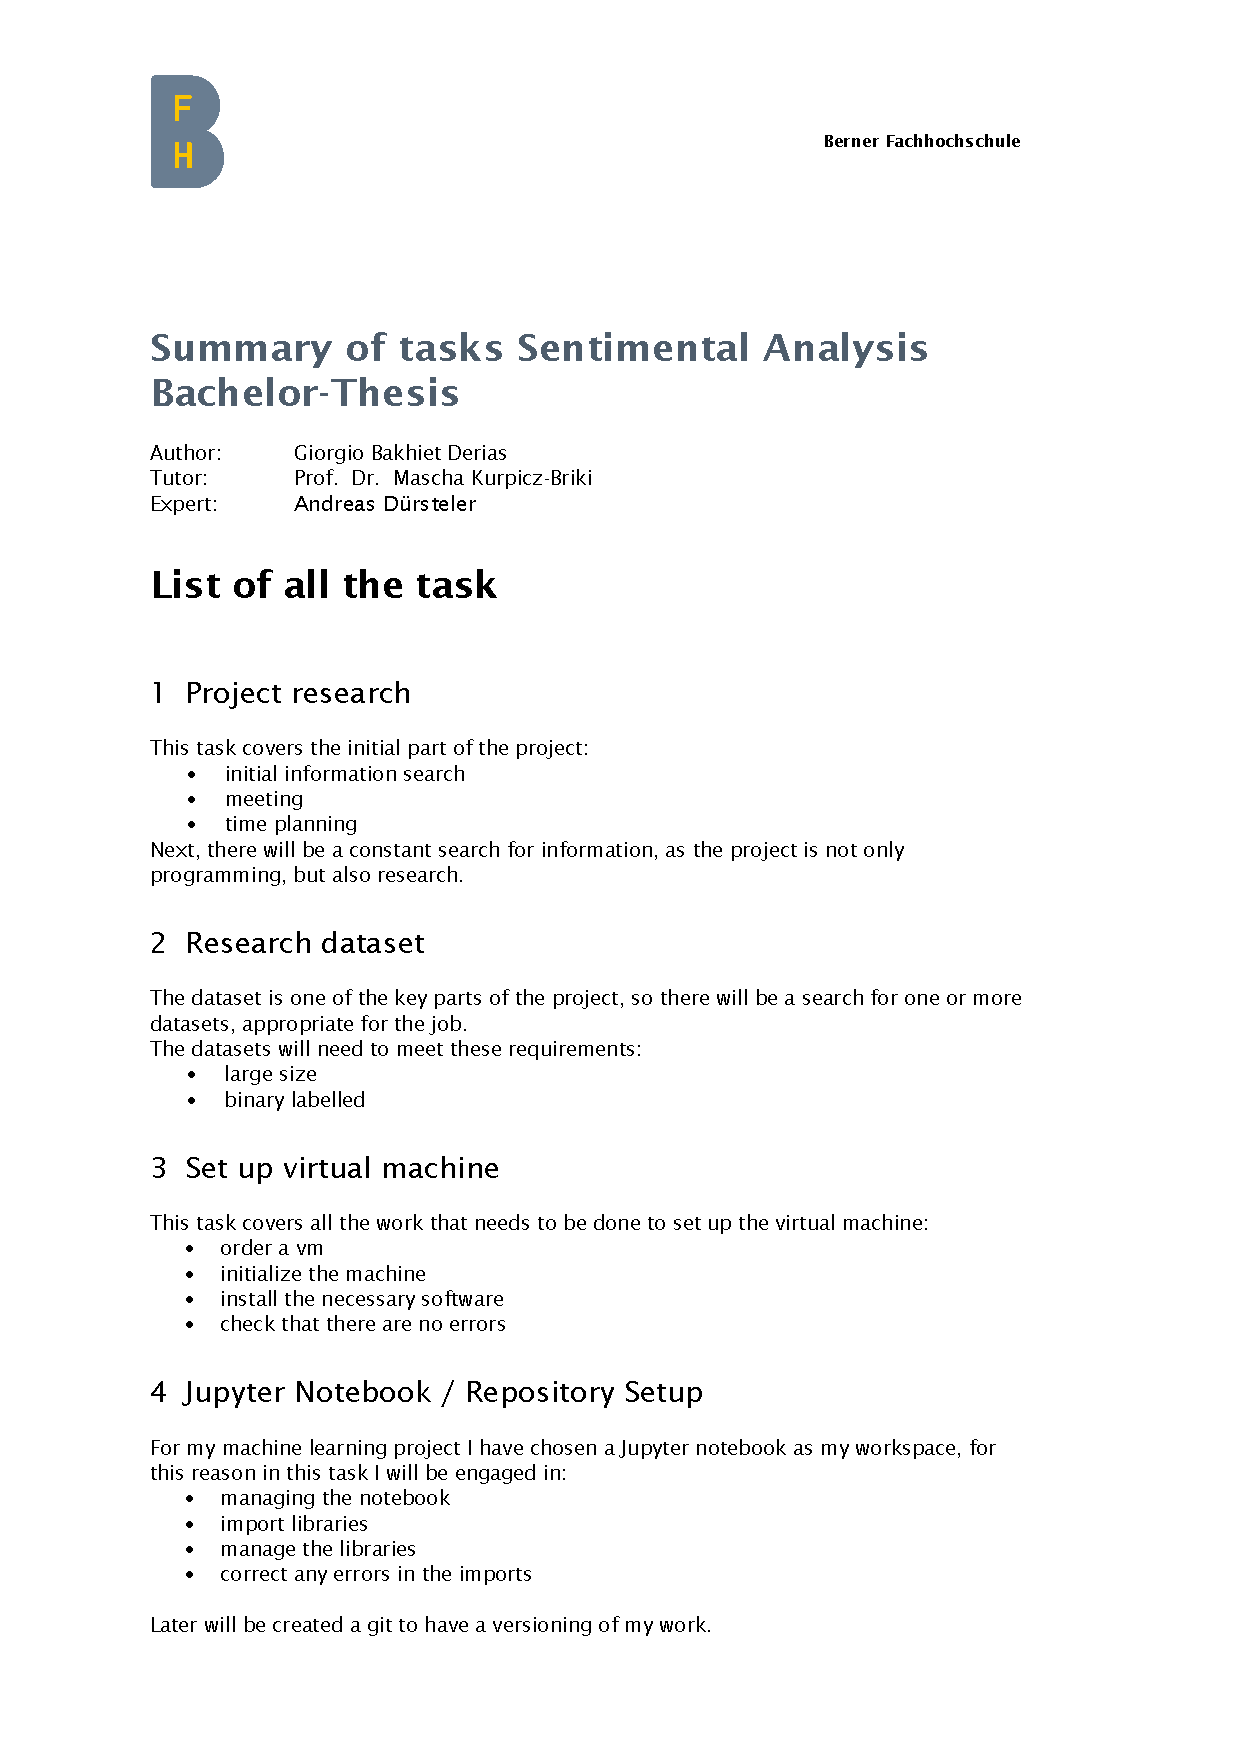
\includepdf[pages=-]{Tasks Giorgio Bakhiet Derias.pdf}
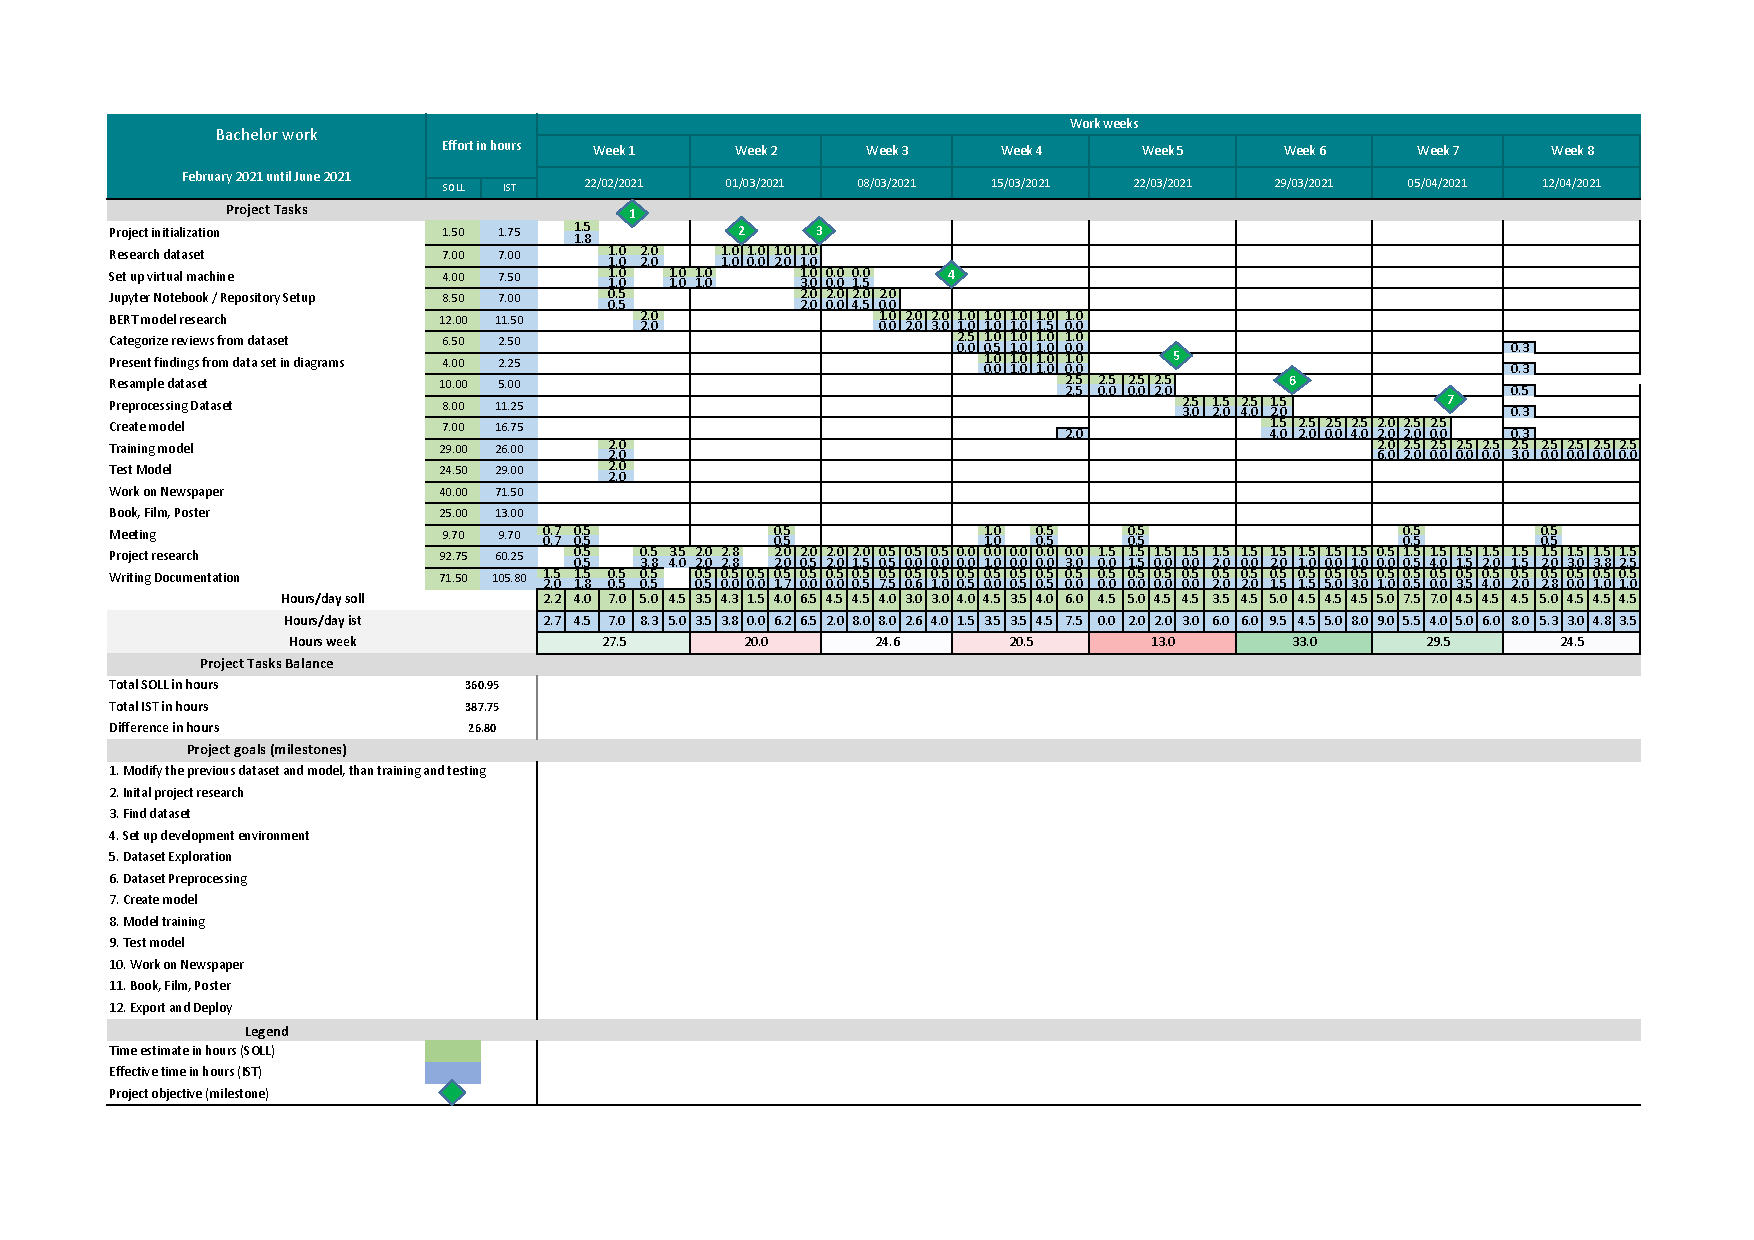
\includepdf[landscape=true]{bachtime1.pdf}
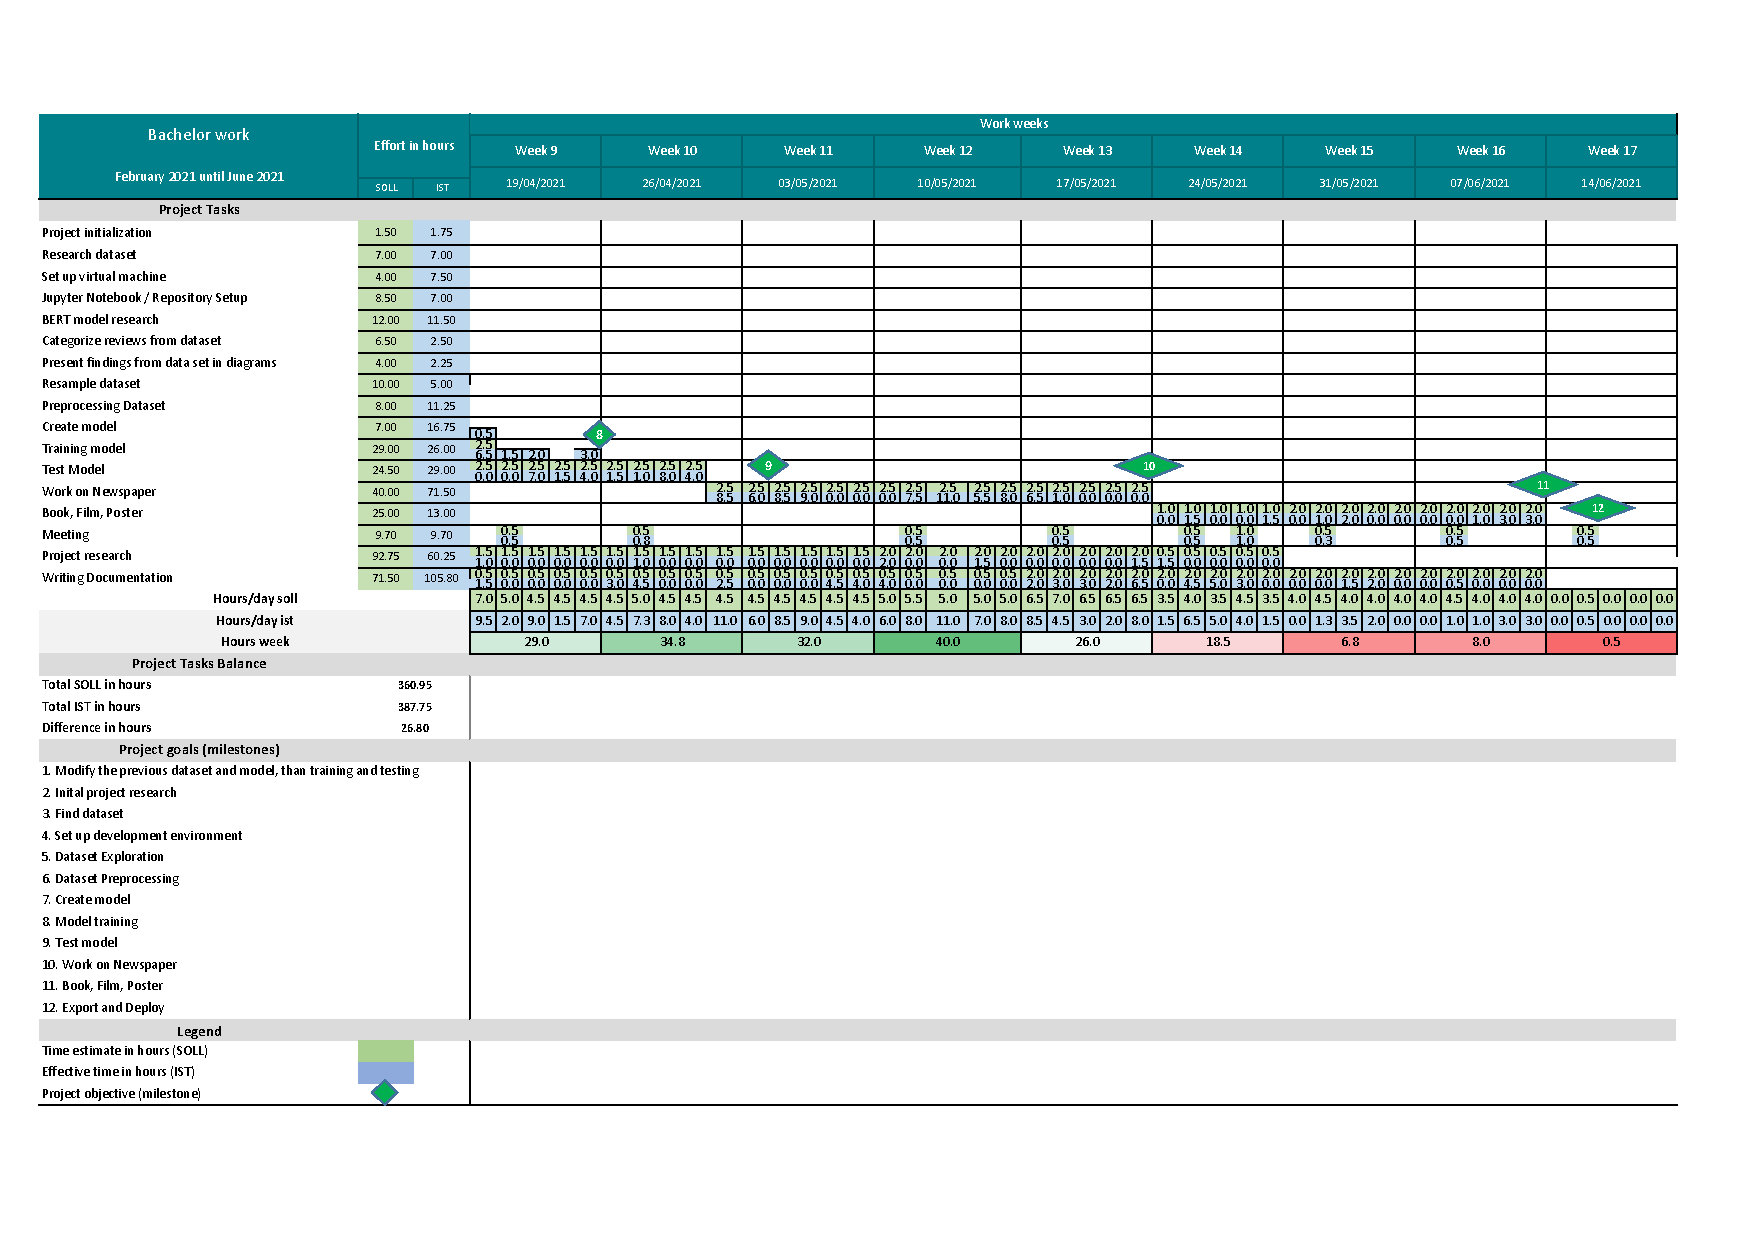
\includepdf[landscape=true]{bachtime2.pdf}
%---------------------------------------------------------------------------
% Index
%---------------------------------------------------------------------------
\clearpage
\phantomsection 
\addcontentsline{toc}{section}{Index}
\printindex
%---------------------------------------------------------------------------
\end{document}
